\documentclass[journal=jpcbfk,manuscript=article]{achemso}

\usepackage{graphicx}
\usepackage{wrapfig}
\usepackage{subcaption}
\usepackage{amsmath} 
\usepackage{siunitx}
\usepackage{booktabs}
\usepackage{gensymb}
\usepackage{xr}

\SectionNumbersOn

\externaldocument[S-]{supporting_information}

\title{Understanding the Nanoscale Structure of Inverted Hexagonal Phase Lyotropic Liquid Crystal Polymer Membranes}
\author{Benjamin J. Coscia}
\affiliation{Department of Chemical and Biological Engineering, University of Colorado Boulder, Boulder, CO 80309, USA}
\author{Joseph Yelk}
\author{Matthew A. Glaser}
\affiliation{Department of Physics, University of Colorado Boulder, Boulder CO, 80309, USA}
\author{Douglas L. Gin}
\affiliation{Department of Chemical and Biological Engineering, University of Colorado Boulder, Boulder, CO 80309, USA}
\alsoaffiliation{Department of Chemistry and Biochemistry, University of Colorado Boulder, Boulder CO 80309, USA}
\author{Xunda Feng}
\affiliation{Department of Chemical and Environmental Engineering, Yale University, New Haven, Connecticut 06511, USA}
\author{Michael R. Shirts}
\email{michael.shirts@colorado.edu}
\affiliation{Department of Chemical and Biological Engineering, University of Colorado Boulder, Boulder, CO 80309, USA}
\begin{document}

  \graphicspath{{./figures/}}
  
  \begin{abstract}
  
  %NOTE: all deleted comments are still in Draft.tex 
  
  Periodic, nanostructured porous polymer membranes made from the cross-linked
  inverted hexagonal phase of self-assembled lyotropic liquid crystals (LLCs) are
  a promising class of materials for selective separations. In this work, we
  investigate an experimentally characterized LLC polymer membrane using
  atomistic molecular modeling. In particular, we compare simulated X-ray
  diffraction (XRD) patterns with experimental XRD data to quantify and
  understand the differences between simulation and experiment.  We find that the
  nanopores are likely composed of 5 columns of stacked LLC monomers which
  surround each hydrophilic core. Evidence suggests that these columns likely
  move independently of each other over longer time scales than accessible via
  atomistic simulation. We also find that WAXS structural features previously
  attributed to monomer tail tilt is likely instead due to ordered tail packing.
  Although this system has been reported as dry, we show that small amounts of
  water are necessary to reproduce all features from the experimental XRD pattern
  due to asymmetries introduced by hydrogen bonds between the monomer head groups
  and water molecules. Finally, we explore the composition and structure of the
  nanopores and reveal that there exists a composition gradient rather than an
  abrupt partition between the hydrophilic and hydrophobic regions. A caveat is
  that the time scales of the dynamics are extremely long for this system,
  resulting in simulated structures that appear too ordered, thus requiring
  careful examination of the metastable states observed in order to draw any
  conclusions. The clearer picture of the nanoscopic structure of these membranes
  provided in this study will enable a better understanding of the mechanisms of
  small molecule transport within these nanopores.

  \end{abstract}

  \section{Introduction}

  More highly selective nanoporous membranes would be extremely useful for
  performing complex aqueous separations with seawater and various types of
  wastewater. For example, Sodium chloride and boron in seawater
  \cite{fritzmann_state---art_2007} and organic micropollutants found in
  municipal and industrial wastewaters \cite{schwarzenbach_challenge_2006}
  represent just a few of the diverse contaminants of water sources. By
  efficiently separating contaminants from feed solutions with highly selective
  membranes, it is possible to reduce the number of required membrane passes and
  post-treatment steps needed for a given filtration process
  \cite{werber_materials_2016}, thus lowering energy requirements. Additionally,
  one can also extract valuable resources from the feed streams. For example,
  flowback water produced during hydraulic fracturing of shale formations
  contains dissolved species such as acetate whose extraction has economic value
  \cite{dischinger_application_2017}.  

  Reverse osmosis (RO) and nanofiltration (NF) are two prevailing membrane
  filtration processes that can be used to separate solutes on the order of 1 nm
  in size and smaller, including ions. However, commercially available amorphous
  RO membranes and porous NF membranes lack uniformity, which severely impacts
  their selectivity \cite{van_der_bruggen_review_2003}. Although scalable, their
  fabrication involves the spontaneous assembly of polymers into disordered
  structures that offer separation pathways that are tortuous and polydisperse in
  size \cite{werber_materials_2016}. Tortuosity increases the effective length
  that a solute must travel, while pore size polydispersity limits membrane
  selectivity.

  Ordered, nanostructured porous membrane materials have become an increasingly popular
  research area for aqueous separation applications because they offer the
  ability to control pore architecture at the molecular scale, thereby
  permitting the design of solute-specific separation membranes
  \cite{humplik_nanostructured_2011}. However, their development has been limited
  by the ability to synthesize and scale various technologies. Graphene sheets
  are atomically thick, which results in excellent water permeability but defects
  during manufacturing severely impact selectivity
  \cite{cohen-tanugi_multilayer_2016}.  Molecular dynamics (MD) simulations of
  carbon nanotubes have shown promise \cite{humplik_nanostructured_2011}, but
  synthetic techniques are unable to achieve scalable alignment and pore
  monodispersity \cite{hata_water-assisted_2004,maruyama_growth_2005}.
  Consequently, there is a need for new materials that could provide scalable
  nanostructured porous membranes. 

  Preliminary evidence has shown that cross-linked lyotropic liquid crystal
  (LLC) membranes can be produced at moderate scale and may be capable of
  performing highly selective separations. LLCs are amphiphilic molecules that
  have the ability to self-assemble into porous nanostructures
  \cite{smith_ordered_1997} and can be cross-linked to create mechanically strong
  membrane films with periodic pores on the order of 1 nm in diameter
  \cite{zhou_supported_2005}. Unlike the pores in most commercial NF membranes,
  polymeric LLC membrane pores are uniform in size because they are formed by
  self-assembly. Since LLC polymer membranes lack an appreciable pore size
  distribution, they inherently exhibit high selectivity due to their strict
  molecular weight cut-off (MWCO)~\cite{zhou_supported_2005}. Additionally, the
  LLC monomers examined in this paper are salts, and therefore lead to Donnan
  exclusion of ions in solution. The membrane gains a net surface charge when
  counterions from the head groups that line the pore walls escape into the feed
  solution in an effort to balance the gradients of concentration and electric
  potential \cite{donnan_theory_1995}.    

  The feasibility of nanostructured LLC polymer membranes for selective
  separations has been demonstrated using LLC monomers that form the type 1
  bicontinuous cubic (Q\textsubscript{I})
  \cite{hatakeyama_water_2011,hatakeyama_nanoporous_2010,carter_glycerol-based_2012}
  and the inverted hexagonal (H\textsubscript{II}) \cite{zhou_supported_2005}
  phases. When separating organic solutes from NaCl, Q\textsubscript{I}-phase
  membrane filtration experiments have shown selectivity 2--3 times higher than
  commercial RO and 6--12 times higher than commercial NF membranes
  \cite{dischinger_application_2017}. When separating a series of various sized
  dyes, the H\textsubscript{II}-phase membrane showed complete rejection of dyes
  bigger than 1.2 nm in size \cite{zhou_supported_2005}. 

  The H\textsubscript{II}-phase pore geometry (Figure~\ref{fig:assembly}) has a
  higher theoretical capacity for transport than the Q\textsubscript{I} phase.
  The H\textsubscript{II} phase forms at room temperature in the presence of
  ca.~10 wt\% water and consists of hexagonally packed, hydrophilic pore
  columns\cite{smith_ordered_1997}. In the absence of water, neat monomer will
  form the same hexagonal columnar structure which, in the literature, has been
  referred to as the Col\textsubscript{h} thermotropic
  phase\cite{feng_scalable_2014}. Q\textsubscript{I}-phase membranes consist of
  a tortuous network of three dimensionally interconnected pores that prevent
  optimal through-plane transport. In contrast, the densely packed, non-tortuous
  and uniform sized pores of H\textsubscript{II}-phase membranes represent the
  ideal geometry for achieving high solute
  flux\cite{matyka_tortuosity-porosity_2008}. However, the hexagonally packed LC
  domains of the H\textsubscript{II}-phase generally form mutually unaligned
  domains, which hurts membrane permeability. This domain scale misalignment had
  inhibited further development of this technology, and research efforts were
  focused on the Q\textsubscript{I} phase, whose geometry does not require
  alignment~\cite{zhou_new_2007}. 

  However, recently researchers have learned how to macroscopically align the
  hexagonal domains which has revived research into H\textsubscript{II}-phase LLC
  polymer membranes. In 2014, Feng et al.~showed that one can align Col\textsubscript{h}
  domains, created by the ``dry" monomer Na-GA3C11, using a magnetic field
  with subsequent cross-linking to lock the structure in
  place\cite{feng_scalable_2014}. In 2016, Feng et al.~showed that one could
  also obtain the same result by confining the neat monomer between PDMS or glass
  substrates since hexagonal mesophases preferentially anchor perpendicular to
  both surfaces\cite{feng_thin_2016}. Current experimental efforts are focused
  on extending the method to the H\textsubscript{II} phase and characterizing
  the performance of these newly aligned systems.

  \begin{figure}
	\centering
	\begin{subfigure}{.3\textwidth}
		\centering
		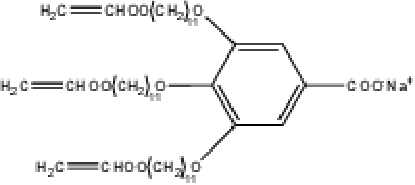
\includegraphics[width=\textwidth]{NaGA3C11.pdf}
		\caption{}~\label{fig:monomer}
	\end{subfigure}
	\begin{subfigure}{.3\textwidth}
		\centering
		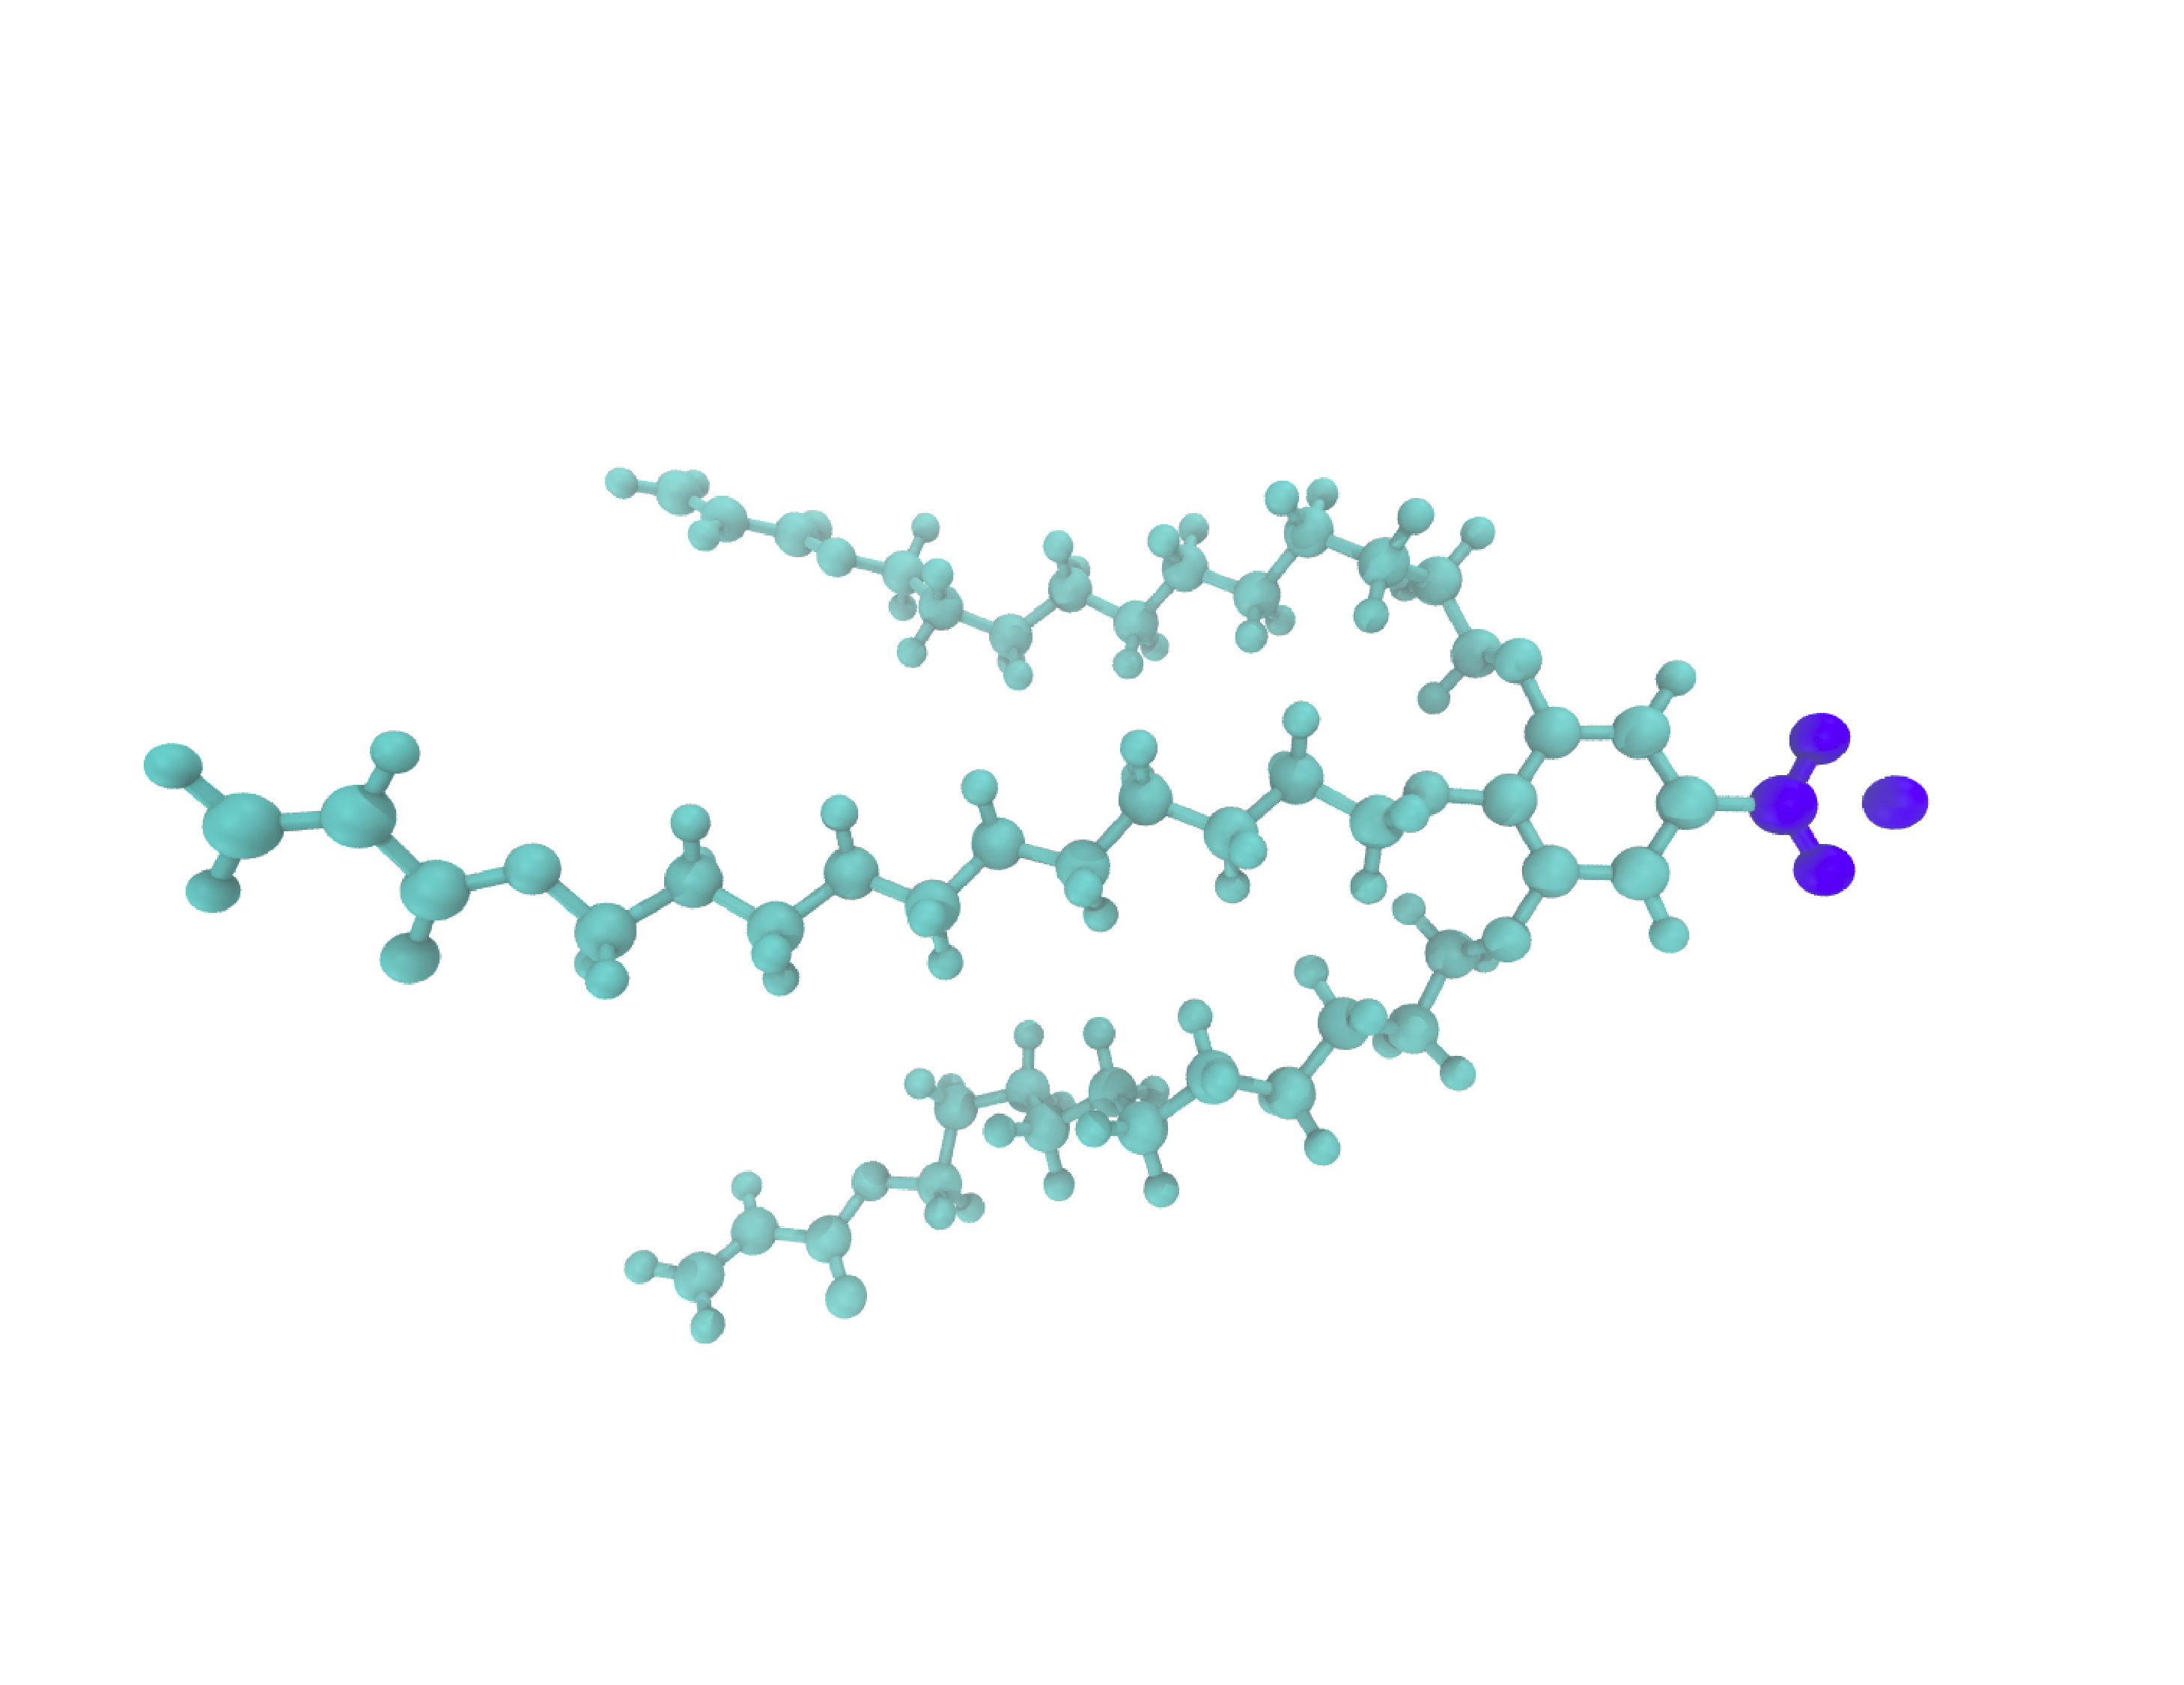
\includegraphics[width=\textwidth]{monomer_twocolor.pdf}
		\caption{}~\label{fig:atomistic_monomer}
	\end{subfigure}
	\begin{subfigure}{0.3\linewidth}
		\centering
		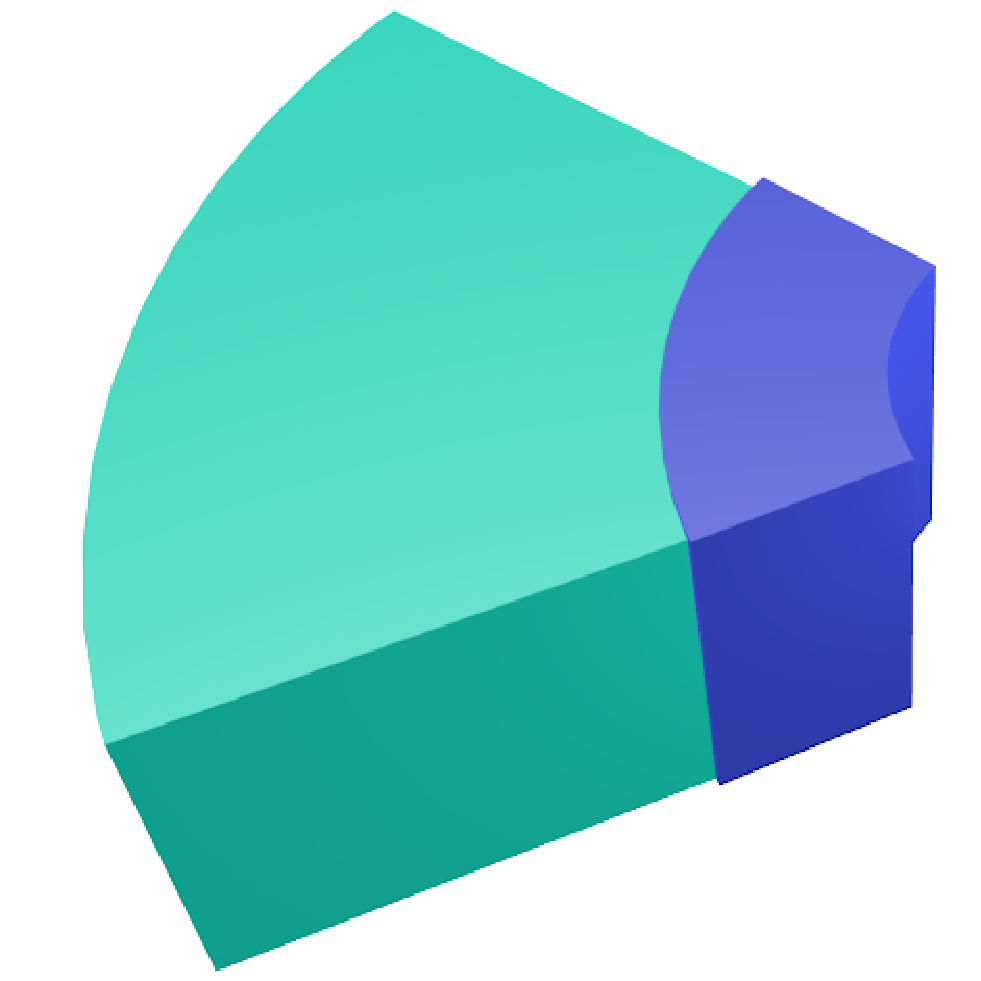
\includegraphics[width=0.6\textwidth]{wedge_thick.pdf}
		\caption{}~\label{fig:wedge}
	\end{subfigure}
		\begin{subfigure}{0.4\linewidth}
		\centering
		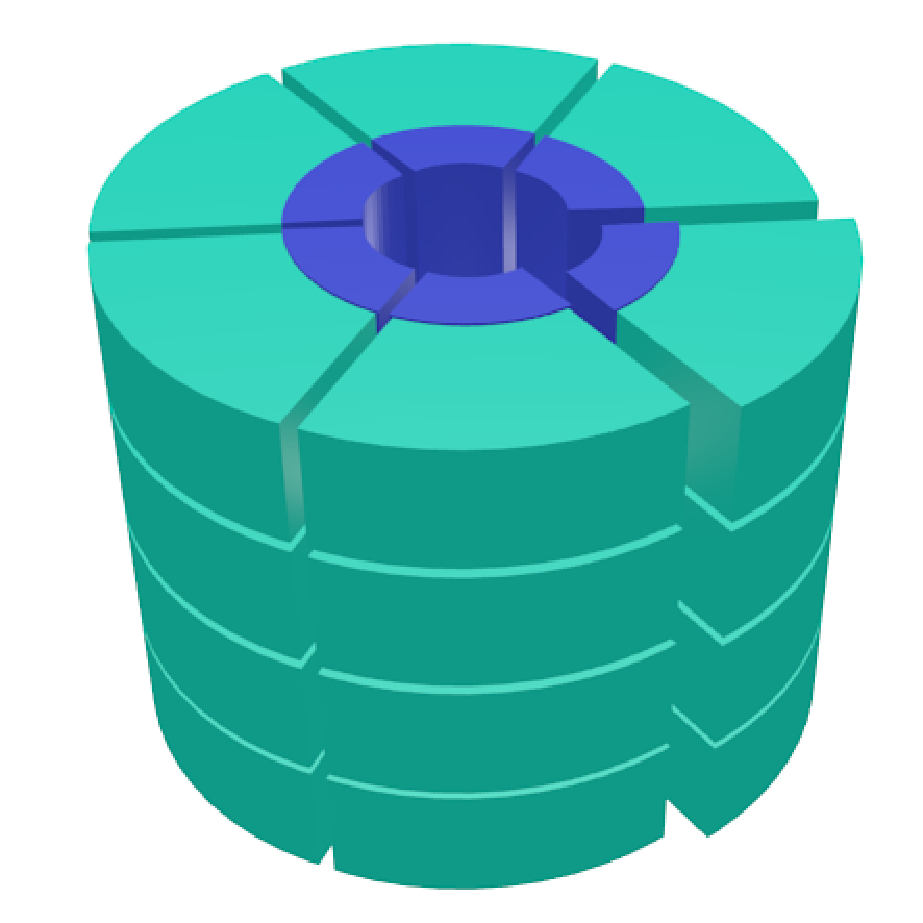
\includegraphics[width=0.6\textwidth]{columns.pdf}
		\caption{}~\label{fig:wedge_layer}
	\end{subfigure}
	\begin{subfigure}{0.4\linewidth}
		\centering
		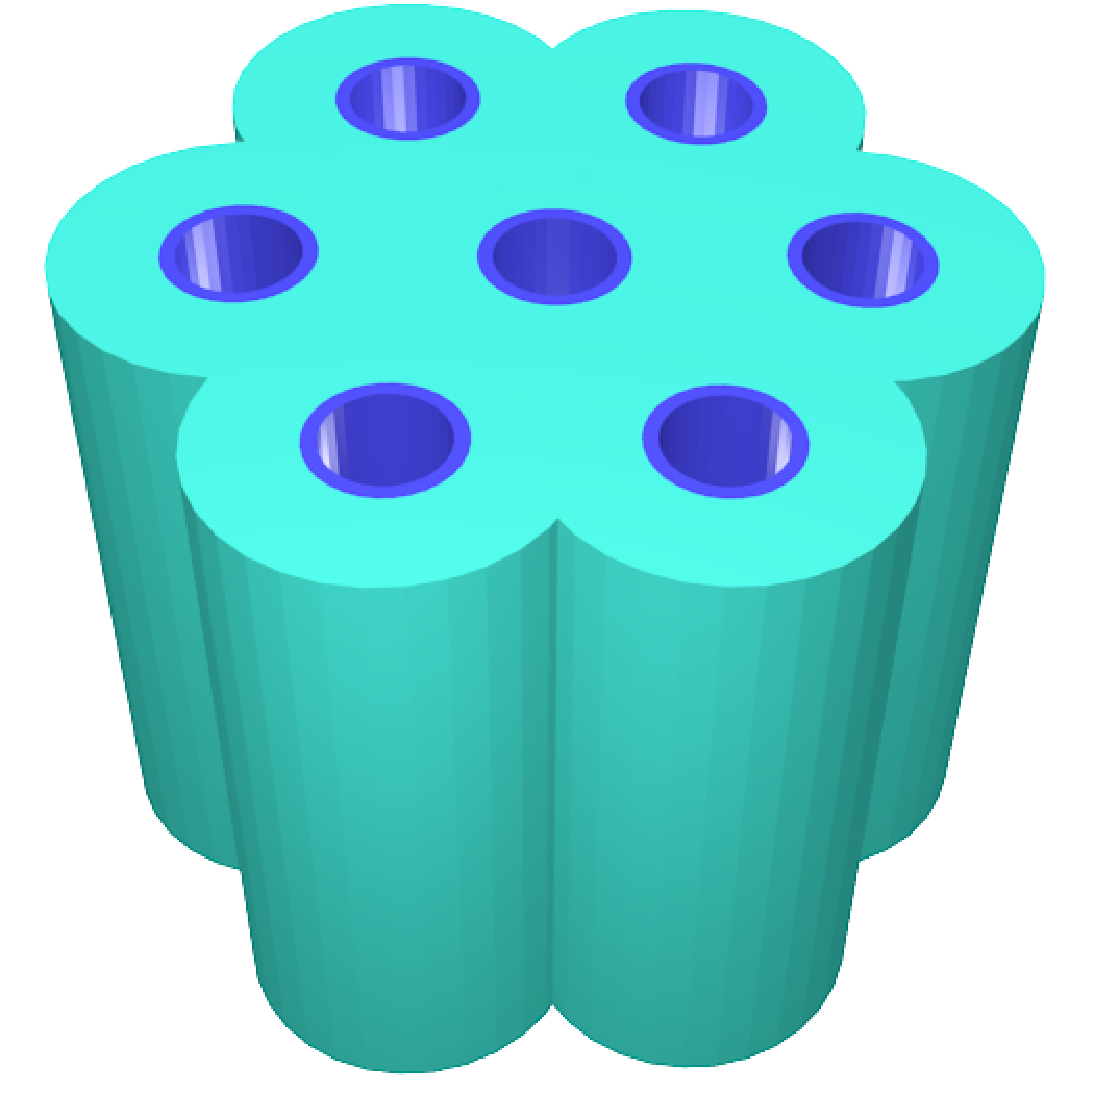
\includegraphics[width=0.6\textwidth]{hexagonal_packing.pdf}
		\caption{}~\label{fig:hex_packing_simple}
	\end{subfigure}
	\caption{(a) The LLC monomer Na-GA3C11 (b) rendered atomistically (c)
	exhibits wedge-like character. (d) Monomers stack on top of each other to
	create columns with short range order, then assemble into pores with 
	hydrophilic head groups (blue) facing towards the pore center. (e) The 
	pores assemble into hexagonally packed columnar mesophases.}~\label{fig:assembly}
  \end{figure}

  Our current understanding of the molecular details of resulting LLC polymer membranes'
  nanostructure is not sufficient to be able to precisely design them for
  specific separations. Dischinger et al.~attempted to use an empirical model
  that correlates the physiochemical properties of the counterion used in a 
  Q\textsubscript{I}-phase LLC membrane to solute rejection\cite{dischinger_effect_2017}.
  Although their model showed some qualitative agreement with experiment, the
  quality of fit of their model was limited due to complex solute-membrane 
  interactions that could not easily be modeled. Additionally, they observed
  an unexpected discrepancy in the relationship between uncharged solute
  rejection and water permeability, which will require a more in-depth knowledge of
  the difference between solute and solvent transport.
  
  Over the past 20 years, H\textsubscript{II}-phase LLC
  polymer membrane studies have been limited primarily to the Na-GA3C11 monomer with some
  characterization done after minor structural modifications. For example, 
  Resel et al.~varied the length of the monomer tails and the counterion used and observed its effect
  on pore spacing \cite{resel_structural_2000}.  In a later study of rejection
  performance, it was shown that membranes formed by cross-linked Na-GA3C11 in
  the H\textsubscript{II} phase cannot separate solutes less than 1.2 nm in
  diameter because the pores are too large \cite{zhou_supported_2005}. We do not
  yet understand how to controllably reduce the effective pore size or how to
  tune the chemical environment in the nanopores of this or related materials for
  small molecule separations. The only source of predictive modeling for LLC
  systems have been macroscopic models that likely do not adequately describe
  transport at these length scales \cite{hatakeyama_water_2011}. Modeling with
  molecular detail could provide sufficient information about the mechanisms and
  chemical features to better inform experimental design of similar
  nanostructured membranes. 

  A molecular-level understanding of LLC polymer membrane structure, enabled by
  molecular dynamics (MD) simulations, can provide guidelines to reduce the large
  chemical space available to design monomers for creation of separation-specific
  membranes. Useful molecular-level modeling should incorporate a detailed
  picture of the nanoscopic pore structure, which is crucial to understanding the
  role of monomer structure in solute transport and membrane design.  Atomistic
  MD simulations can provide the required level of detail (Figure
  \ref{fig:detail}), assuming the force fields are sufficiently accurate.  With
  such an atomistic model, we can directly observe molecular-level solute
  transport and suggest governing mechanisms. We can also observe how the choice
  of head group interacts with solutes of interest. In addition, we can
  interchange counterions which may influence both the pore size and the strength
  of the Donnan potential. 

  In this study, we achieve a more realistic atomistic description of
  hexagonal LLC polymer membranes than, to our knowledge, has ever previously
  been created, and explore what new structural information can be gained and
  what structure hypotheses are supported by this model. We validate the results
  using as much experimental information as possible. We are most interested in
  reproducing the conclusions about structure drawn from small-angle X-ray
  scattering (SAXS) and wide-angle X-ray scattering (WAXS) experiments, as well
  as in matching ionic conductivity measurements \cite{feng_thin_2016}.

  \begin{figure}[!htb]
  \centering
	\begin{subfigure}{0.45\linewidth}
		\centering
		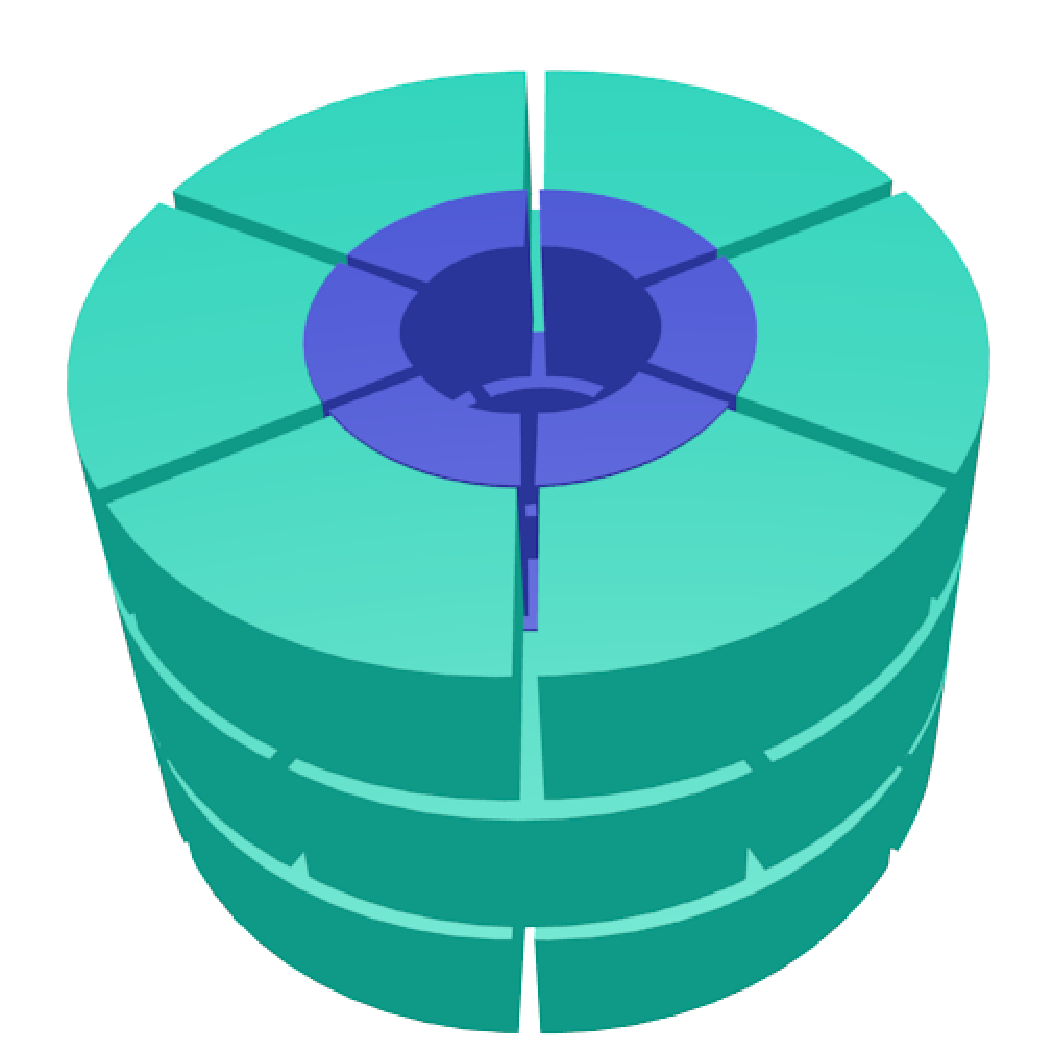
\includegraphics[width=0.6\textwidth]{cartoon_pore.pdf}
		\caption{}~\label{fig:undetailed_pore}
	\end{subfigure}
	\begin{subfigure}{0.45\linewidth}
		\centering
		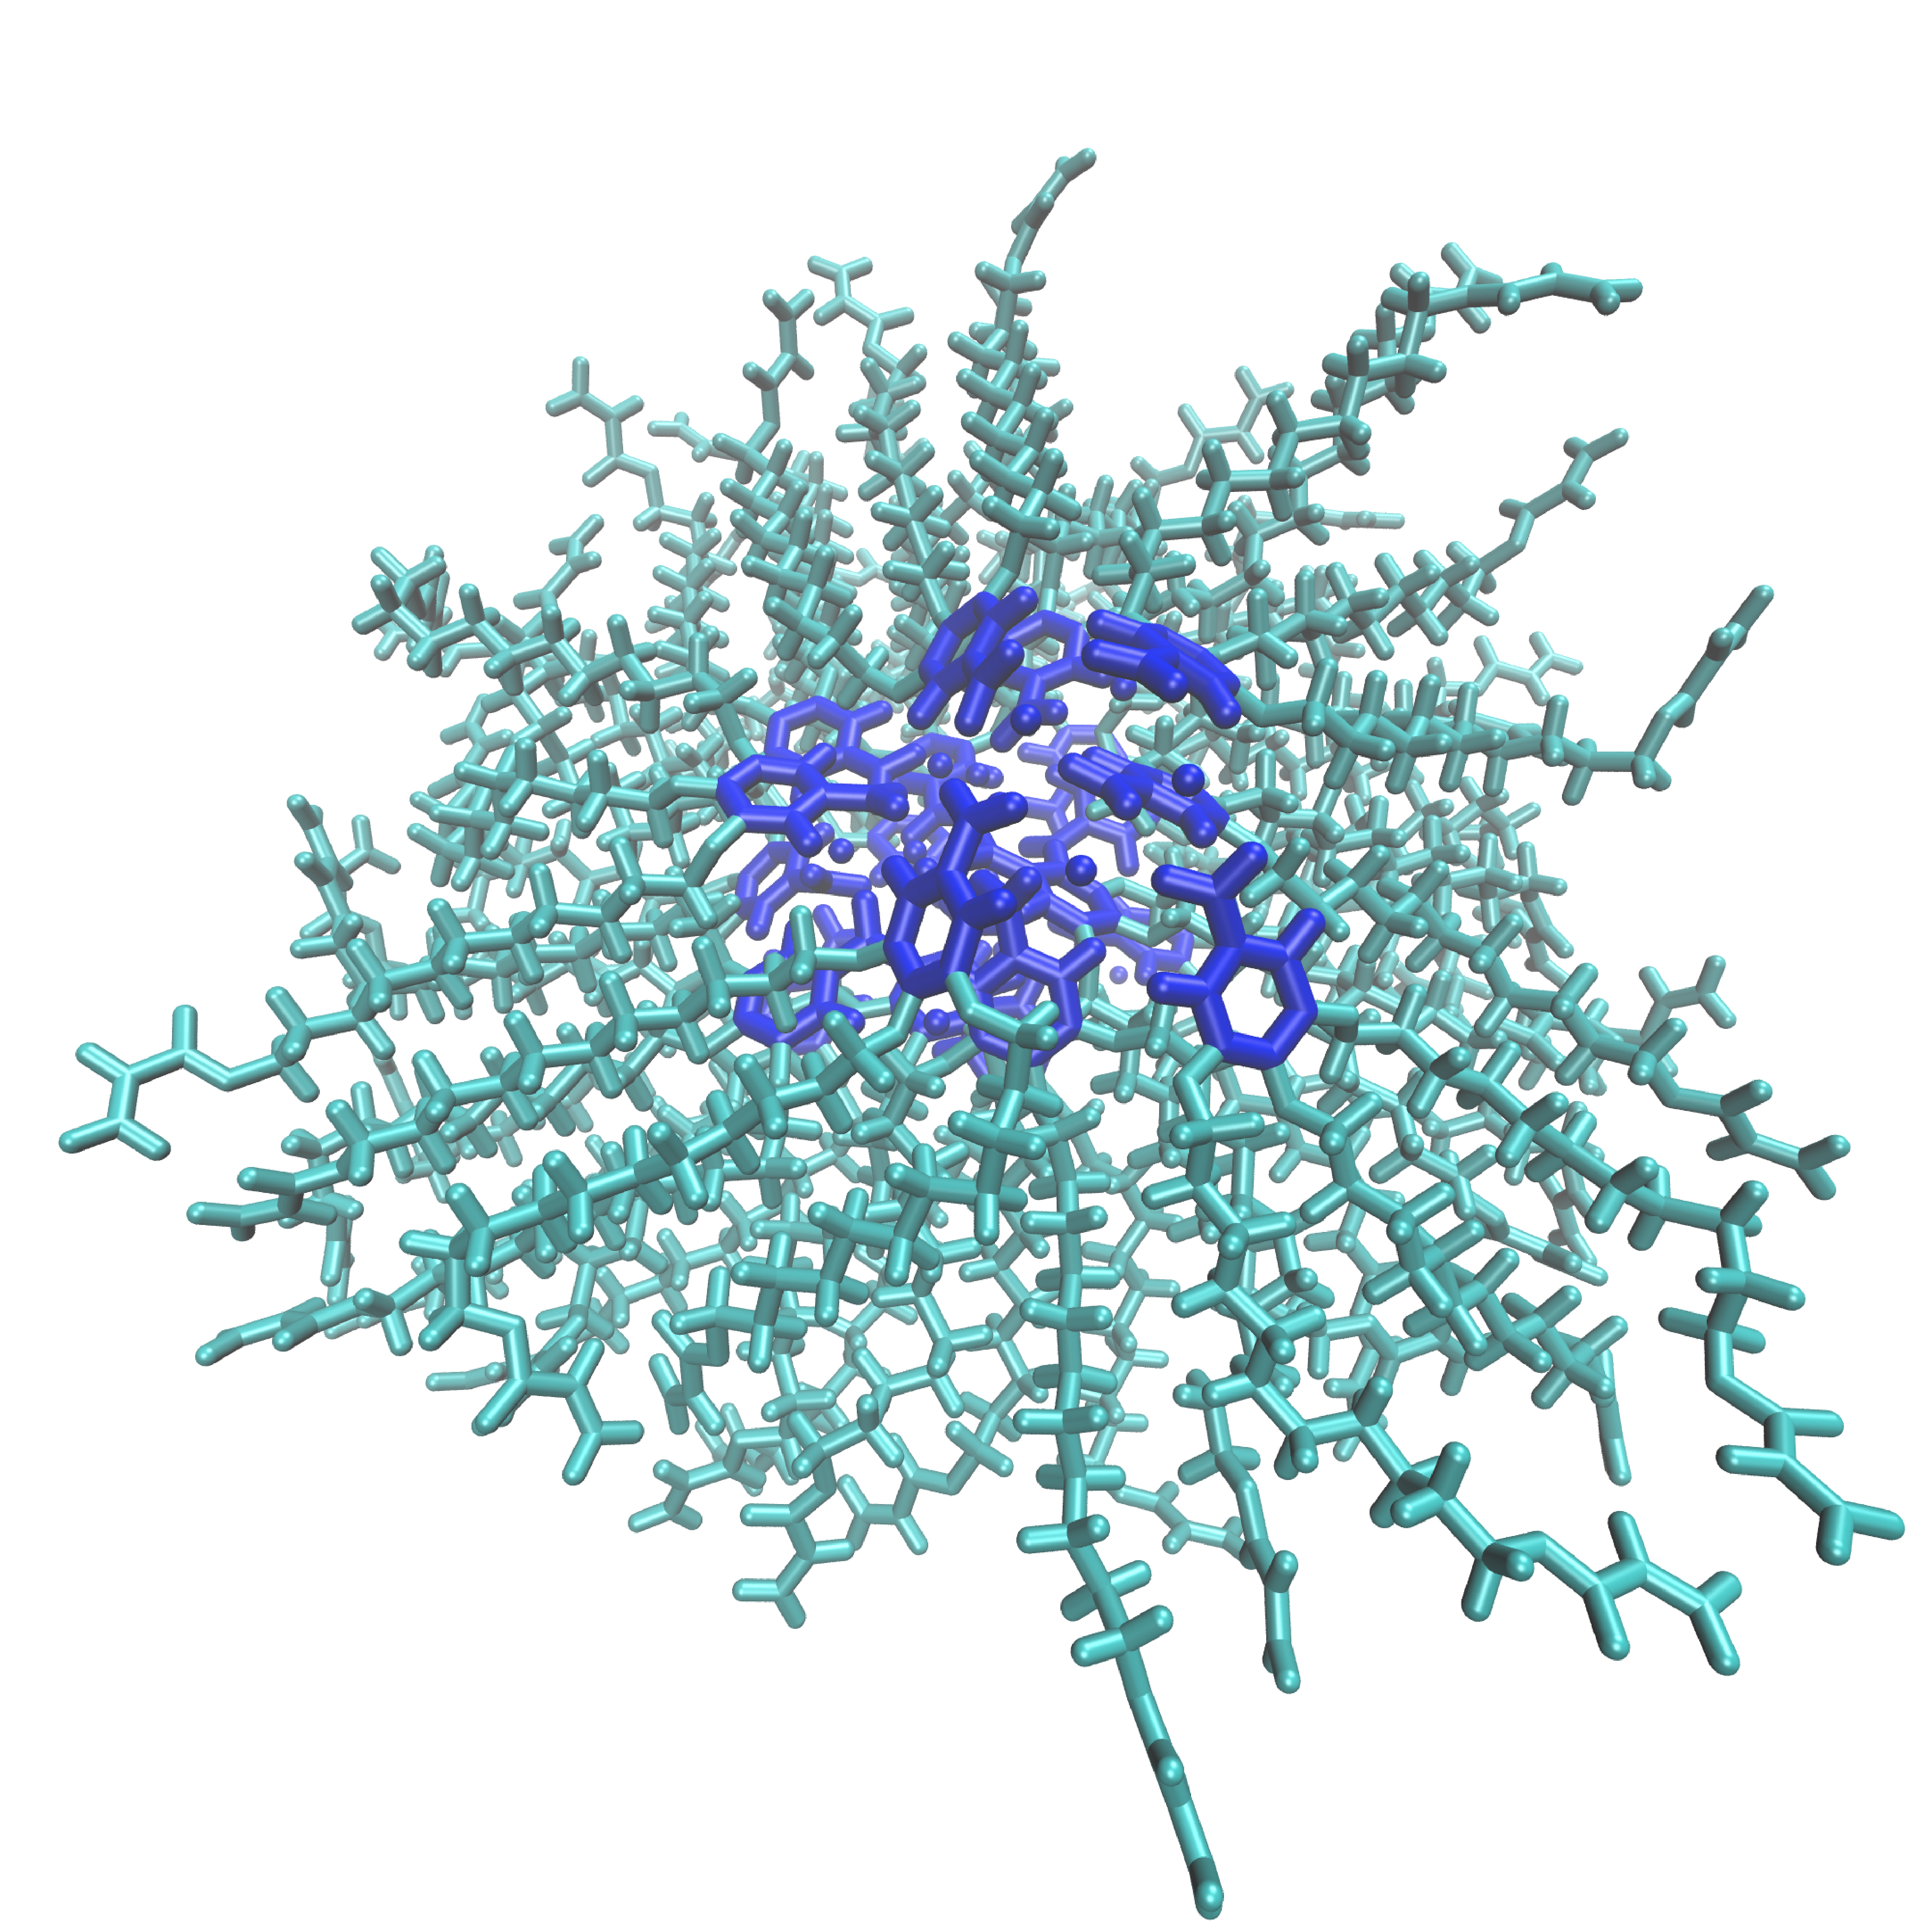
\includegraphics[width=0.6\textwidth]{detailed_pore.pdf}
		\caption{}~\label{fig:detailed_pore}
	\end{subfigure} 
    \caption{(a) Previous understanding of the pores are essentially speculations 
    based on limited chemical and experimental data. (b) We use detailed molecular 
    modeling in this paper in order to appropriately model the pore's complex architecture,
    which is crucial to understanding the mechanism of solute transport. In both 
    pictures, the head group region is colored blue and the tail region is colored cyan.}~\label{fig:detail}
  \end{figure}
 
  In this paper, we perform molecular modeling of the Col\textsubscript{h}
  thermotropic (i.e., solvent-free) assembly formed by Na-GA3C11. Compared to the
  lyotropic (i.e, solvent-containing) H\textsubscript{II} phase, the
  Col\textsubscript{h} phase is a simpler starting point. The system is not
  assembled in aqueous phase which allowed us to simulate longer timescales by
  omitting the solvent in the simulations, and there exists detailed experimental
  characterization of the fully aligned state, including 2D-WAXS patterns
  (Figure~\ref{fig:WAXS}) that are useful for reconstructing structural data. 
  
  There are five major features of interest present in the 2D experimental
  WAXS pattern shown in Figure~\ref{fig:WAXS}.

  \begin{enumerate} 
  
	\item \textit{R-$\pi$}: The location of the first is at $q_z$ = 1.7
	\AA$^{-1}$, corresponding to a real space separation of 3.7 {\AA}. Previous
	work attributes this reflection to $\pi$-$\pi$
	stacking between aromatic rings in the direction perpendicular to the membrane
	plane, or $z$-axis \cite{feng_scalable_2014}. For simplicity, we will refer to
	this reflection as R-$\pi$.
 
	\item \textit{R-double}: A weak intensity line, located at exactly half
	the $q_z$ value of R-$\pi$ ($q_z$ = 0.85 \AA$^{-1}$), corresponds to real
	space periodicity of 7.4 \AA. Since this reflection corresponds to double
	the spacing of R-$\pi$ in real space, we will refer to it as R-double. 
	R-double has been previously interpreted as 2\textsubscript{1} helical ordering of aromatic
	rings along the $z$-axis\cite{feng_scalable_2014}.

	\item \textit{R-alkanes}: A low intensity ring located at $|\mathbf{q}|$ = 1.4
	\AA$^{-1}$ marks the third major reflection of interest. The real space
	separation corresponds to 4.5 \AA~which is characteristic of the average
	spacing between packed alkane chains \cite{mcintosh_organization_1980}. We will
	call this reflection R-alkanes.

	\item \textit{R-spots}: Within R-alkanes, are four spots of higher
	relative intensity.  Accordingly, we name these reflections R-spots. The
	location of all spots is $\sim37^{\circ}$ from the $q_r$ axis in their
	respective quadrants. In many liquid crystal systems, such spots are explained
	as the result of alkane chains tilted with respect to the membrane
	plane\cite{govind_simple_2001}.
 
	\item \textit{R-pores}: The final significant feature corresponds to the spacing
	and symmetry of the pore columns. The feature, which we named R-pores,
	is characterized by reflections along the equatorial axis defined by $q_z$ = 0.
	The spacing between dots is indicative of the hexagonal symmetry of the packed
	pores. We observe the same information with higher resolution by looking at the
	same system's 1D-SAXS pattern (Fig.~\ref{fig:SAXS}). The location of the
	leading SAXS peak (closest to $q_r$ = 0) is related to the distance between
	pores.
	
  \end{enumerate}

  \begin{figure}[!htb]
        \centering
                \begin{subfigure}[t]{0.495\linewidth}
                \centering
                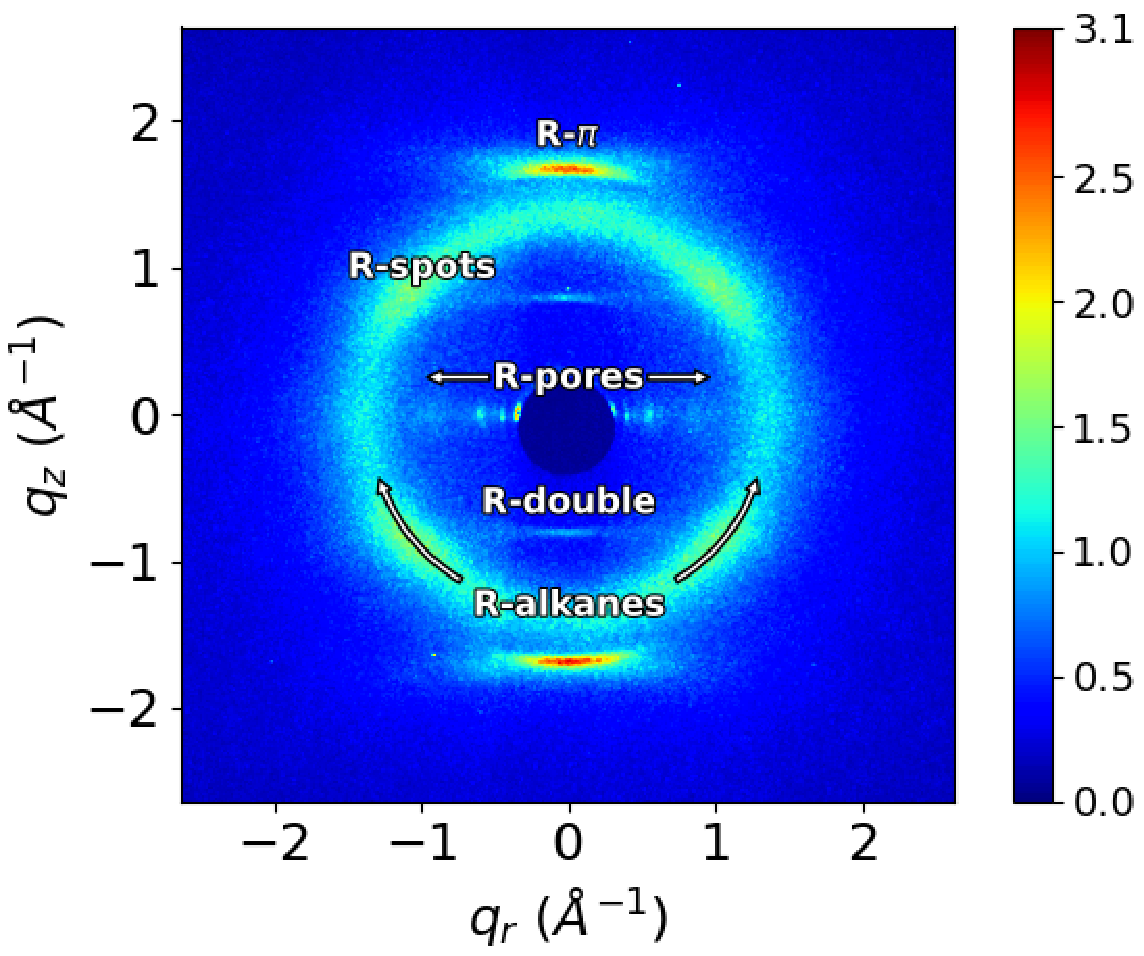
\includegraphics[width=\linewidth]{WAXS_annotated_words.pdf} 
                \caption{}\label{fig:WAXS}
        \end{subfigure}
	\begin{subfigure}[t]{0.38\linewidth}
                \centering
                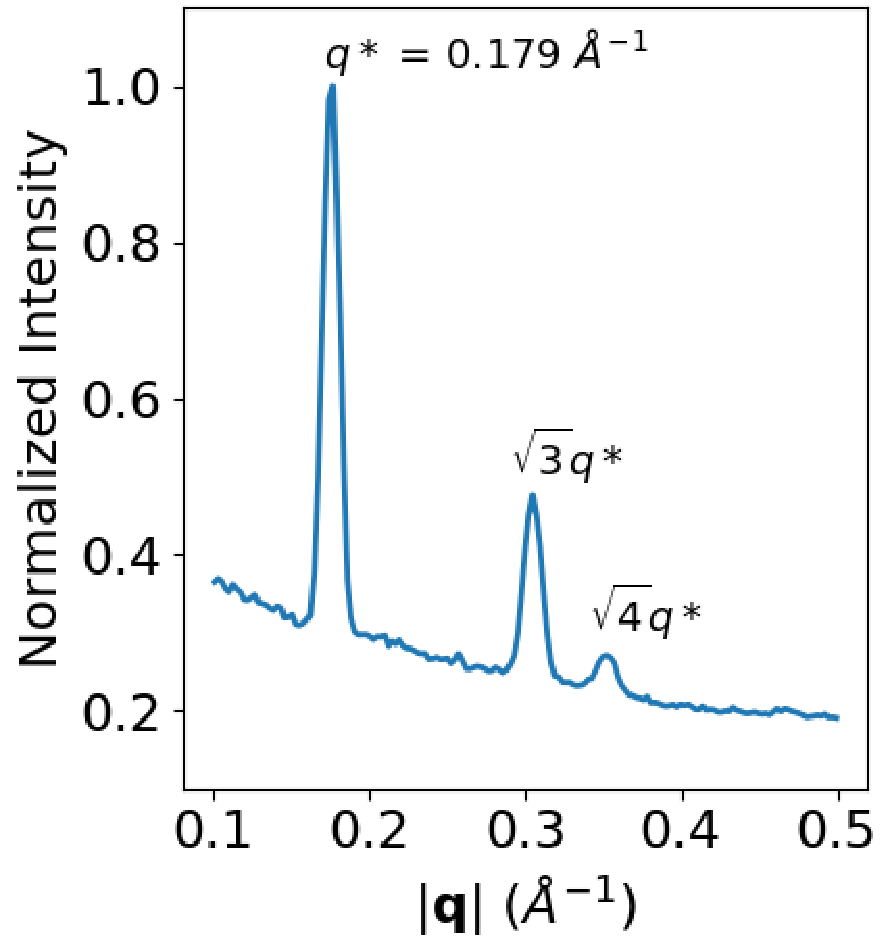
\includegraphics[width=\textwidth]{SAXS.pdf}
                \caption{}\label{fig:SAXS}
        \end{subfigure}
	\caption{(a) 2D-WAXS gives details about repeating features on the
		order of angstroms. Experimentalists have explained each of the 5 major
		reflections present as follows: (R-$\pi$) Aromatic head groups $\pi-\pi$ stack
		3.7 \AA~apart. (R-double) Monomers arrange vertically in a 2\textsubscript{1}
		helix. (R-alkanes) Alkane chain tails pack 4.5 \AA~apart. (R-spots) Monomer
		tails are tilted with respect to the membrane plane. (R-pores) As derived from
		SAXS, the pores are spaced 4.12 nm apart and pack hexagonally (b) (Reproduced
		from Ref.\citenum{feng_thin_2016}) The repeat spacing in the 1D-SAXS
		scattering pattern is characteristic of hexagonal packing. The leading peak,
		q*, represents the distance between the d\textsubscript{100} planes, which translates 
                into a distance between pore centers of 4.12 nm.} 
	\label{fig:SWAXS}
 \end{figure}
  
 Despite having structural data, there is still information which experiment
 cannot definitively answer. Specifically, we want to know:
 \begin{enumerate}
    \item What is the density of monomers that pack around each hydrophilic core? 
    \label{point:monomernum}

	Authors often describe this and similar systems as being made up of
	stacked monomer layers. A simple molecular simulation study of a similar
	molecule suggested that there are 4 monomers in each layer. Their estimation is
	based on a simulated system containing only 16 total monomers which likely does
	not sufficiently model the chemical environment present in the real
	system.~\cite{zhu_methacrylated_2006}. A separate calculation based on the
	volume of the liquid crystal monomers proposes that there are seven monomers in
	each layer~\cite{resel_structural_2000}. 

	We are careful to avoid the term ``layers" since many liquid
	crystalline systems have long range order in 1 or 2 spatial dimensions and
	short range order in the other dimensions.~\cite{chaikin_principles_1995}  %
	page 58 In the system we are studying, there are long-range 2D correlations in
	the hexagonal array of pores ($xy$ plane) and short range $z$-direction
	correlations within stacked columns of monomers. In this study, we use
	atomistic molecular modeling to study how the system's structure is affected by
	the density of these monomer columns that surround each pore's hydrophilic
	core. 

	\item What structural motif best matches experimental 2D-WAXS patterns?\label{point:xrdmatch}

	On the short timescales accessible to MD (even the 100's of nanoseconds
	of simulation performed here are short compared to experimental timescales), we
	observe distinct metastable configurations which depend on starting
	configuration. We simulated X-ray diffraction (XRD) patterns of our system and
	compared them to experimental 2D WAXS patterns (Figure~\ref{fig:WAXS}) so that
	we ensure our model creates a nanoscopic chemical environment maximally
	consistent with experiment within the constraints of our force field. Using
	this approach, we are able to confirm some previous interpretations	of the
	WAXS pattern and refute others. 

        \item Is it necessary to include any water in order to appropriately model the 
        Col\textsubscript{h} phase? \label{point:water}

	While the Col\textsubscript{h} phase is described as dry, it is likely
	that small amounts of ambient water are absorbed into the system. The
	hydrogen-bonding network formed by the water may play a role in structuring the
	pore. We used simulated XRD patterns to uncover any meaningful structural
	difference between a ``dry" and a ``wet" system.

	\item What is the detailed atomistic structure of the pores?\label{point:composition}

	The limited picture that experiment provides tells us that there are hexagonally packed, 
	hydrophilic regions where transport is likely to occur. One may instinctively imagine these 
	regions as tube-like pathways with well-defined boundaries. We explored the composition
	of the pores, the partition between the hydrophilic and hydrophobic regions, and its 
	sensitivity to initial configuration, including both dry and wet systems. 

  \end{enumerate}

  \section{Methods}
 
  \subsection{Source code}

  Python scripts used to set up systems and conduct post-simulation trajectory analysis are
  available online at \texttt{https://github.com/bencoscia/llcsim}. The python scripts used
  to simulated XRD patterns are publicly available online at \\
  \texttt{https://github.com/joeyelk/MD-Structure-Factor}. Additional details are available in 
  Section \ref{S-section:python_scripts} of the Supporting Information (SI).
  
  \subsection{Monomer Parameterization}\label{method:parameterization}

  We parameterized the interaction potential for the liquid crystal monomer 
  Na-GA3C11 using the Generalized AMBER Force Field (GAFF) 
  \cite{wang_development_2004} with the Antechamber package \cite{wang_automatic_2006} 
  provided with AmberTools16 \cite{case_ambertools16_2016}. We assigned atomic
  charges using the am1bccsym method of \texttt{molcharge} shipped with QUACPAC
  from Openeye Scientific Software. We ran all molecular dynamics simulations 
  using GROMACS 2016 \cite{bekker_gromacs:_1993,berendsen_gromacs:_1995,van_der_spoel_gromacs:_2005,hess_gromacs_2008}.

  We generated an ensemble of characteristic, low-energy vacuum monomer
  configurations by applying a simulated annealing process to a
  parameterized monomer. We cooled monomers from 1000 K to 50 K over 10
  ns. We randomly pulled a low energy configuration from the
  trajectory then reassigned charges using \texttt{molcharge}. Using the new
  charges, we annealed the monomer system again and pulled a random monomer
  configuration from the trajectory which we used for full system
  construction. Section \ref{S-section:parameterization} 
  of the SI provides further detail of the parameterization process.

  \subsection{Unit Cell Preparation}\label{method:unitcell_build}

  The time scale for self-assembly of monomers into the hexagonal phase is
  unknown and likely outside of a reasonable length for an atomistic simulation,
  requiring a more efficient way to build the system. Previous work has shown
  that a united-atom model of an LLC can self-assemble into the
  H\textsubscript{II} phase configuration in $\sim$1000 ns
  \cite{mondal_self-assembly_2013}. We attempted atomistic self-assembly by
  packing monomers into a box using Packmol \cite{martinez_packmol:_2009}.
  Simulations of greater than 100 ns show no indicators of progress towards an
  ordered system (see Section \ref{S-section:self_assembly} of the SI). To bypass
  the slow self-assembly process, we used automated procedures to
  assemble monomers into a structure close to one of a number of hypothesized
  equilibrium configurations (See Figure \ref{S-fig:build_procedure} of the SI).
  These initial structures may result in equilibration into slowly-intercoverting
  metastable states, an issue we will address later in the paper. 

  A typical simulation volume contains four pores in a monoclinic unit cell,
  the smallest unit cell that maintains hexagonal symmetry when extended
  periodically. Each pore is made of columns of stacked monomers with periodic
  continuity along the pore axis, avoiding any edge effects and creating an
  infinite length pore ideal for studying transport. We prefer a small number of stacked
  monomers in order to reduce computational cost and to allow us to look at
  longer timescales. Ultimately, we chose to build a system with 20 monomers
  per column in order to minimize finite size effects with reasonable computational expense 
  and to obtain sufficient resolution when simulating XRD patterns (see further discussion
  in Section \ref{S-section:monomers_per_column} of the SI).
 
  \subsection{Monomer Placement}\label{method:monomer_placement}

  When constructing an initial configuration, there are a number of variables
  which require careful consideration while placing monomers. We find that the
  equilibrium configuration is sensitive to some while insensitive to others. For
  example, we find the starting pore radius, defined as the distance of a chosen
  head group carbon from the pore's central axis, does not influence the
  equilibrium structure if one chooses a reasonable value. The initial distance
  between pores, within a wide range, also has little effect on the equilibrated
  structure. However, one should not start them too close or there will be high
  energy repulsions during early equilibration. We chose a pore radius of 0.5 nm
  and an initial pore spacing of 4.5 nm, $\sim$10\% larger than the experimental
  value of 4.12 nm for our initial configurations. A sensitivity analysis of both
  parameters is presented in the SI, Section
  \ref{S-section:initial_config_dependence}. The distance between vertically
  stacked monomers, the $xy$ position of monomers with respect to vertically
  adjacent monomers, and the number of columns per pore do influence the
  equilibrated structure and require further justification for their choices. We
  rely on experimental data to inform them. 

  We chose the vertical spacing between monomers for the initial configuration
  based on R-$\pi$ and then allowed the system to readjust during equilibration.
  We rotated each monomer so the plane of its aromatic head group would be
  coplanar with the $xy$ plane. We explored three different initial monomer
  spacings. The first is exactly equal to R-$\pi$ with monomers placed so
  aromatic rings stack 3.7 \AA~apart in the $z$-direction. We also extensively
  explored a second system with an initial spacing of 5 \AA. We briefly explored
  a third system with an initial spacing of 10 \AA. However this largest spacing
  yields non-physical behavior which is detailed in the SI, Section
  \ref{S-section:initial_dbwl}. 

  We chose the relative orientation between vertically adjacent monomers in each column 
  based on clues from diffraction data as well as the various known stacking modes of 
  benzene and substituted benzene rings: sandwiched, parallel displaced and T-shaped
  \cite{sinnokrot_estimates_2002}. We ruled out the T-shaped configuration
  because its $\sim$5 \AA~equilibrium stacking distance \cite{sinnokrot_estimates_2002}
  is inconsistent with R-$\pi$. It is also infeasible for the monomers to orient in the 
  T-shaped conformation because of the bulky tail groups. We explored the system's 
  preference towards the sandwiched vs. parallel displaced stacking modes in some detail.
  Both have reported stacking distances near the R-$\pi$ value of 3.7 \AA. Head groups in
  our sandwiched initial configuration stack directly on top of each other while
  head groups in the parallel displaced initial configuration stack with an offset
  of $180^\circ/ncol$ where $ncol$ is the number of columns per pore. See Figure 
  \ref{S-fig:stacking} of the SI for a detailed illustration 
  of the initial configurations in each mode.

  The number of columns per pore is unknown, as stated in Question
  (\ref{point:monomernum}). We tested configurations constructed with a varied
  number of columns per pore. We built systems in the sandwiched and parallel
  displaced configurations with 4, 5, 6, 7 and 8 columns per pore.

  \subsection{Equilibration}\label{section:equilibration}
  
  We developed equilibration schemes for creating dry (i.e. thermotropic LC phase)
  and wet (i.e. LLC phase) configurations.
  Both schemes start with an initial configuration generated according to the
  previous guidelines. For wet systems, we added the desired concentration of
  water to the initial configuration and carried out equilibration in the same
  way as the dry systems. First, we fixed monomer head groups in place using
  position restraints with a force constant of 10$^6$ kJ mol$^{-1}$ nm$^{-2}$. We
  gradually released the position restraints by decreasing the force constants
  over a series of NVT simulations. We allowed the resulting unrestrained
  structure to equilibrate for 5 ns in the NPT ensemble with pressure controlled
  by the Berendsen barostat, followed by NPT equilibration simulations run for at
  least 400 ns using the Parrinello-Rahman barostat. More equilibration details
  are given in Section \ref{S-section:equilibration} of the SI.

  \subsection{Equilibrium Calculations}

  \subsubsection{\textit{Determining equilibration time}}\label{method:equil_time}

  Using equilibrated structures, we carried out various calculations to
  characterize the system. We defined the point at which a system is equilibrated
  based on when the distance between pores stopped changing.  We determined when
  the distances stopped changing by applying the statistical test of Chodera~\cite{chodera_simple_2016},
  implemented as \texttt{pymbar.timeseries.detectEquilibration}, to the time series. Typically, the pore-to-pore
  distance equilibrated between 200 and 350 ns. We used data collected after 
  equilibration to do all subsequent analysis.

  \subsubsection{\textit{Calculation of pore spacing}}\label{method:pore_spacing}

  To calculate the equilibrated pore spacing, we measured the distance between
  pore centers. We located the pore centers by averaging the coordinates of
  sodium ions in their respective pores. We generated pore spacing statistics
  using the bootstrapping technique (See Section \ref{S-section:p2p_stats} of the
  SI). The pore spacings calculated in this way are consistent with one half of
  the $x$ and $y$ box vectors (See Table \ref{S-table:p2p} in the SI). However,
  our method for their calculation does a better job capturing the spread of
  pore-to-pore distances.

  \subsubsection{\textit{Generation of simulated X-ray diffraction patterns}}\label{method:xrd}
  
  We generated simulated XRD patterns based on atomic coordinates in order to
  make a direct experimental comparison. We modeled all atomic coordinates as
  Gaussian spheres of electron density whose maximum and width are defined by
  each atom's atomic number and electronic radius respectively. A three dimensional
  Fourier transform of the array of electron density results in a three
  dimensional structure factor which represents the unit cell in reciprocal
  space. The experimental WAXS measurement was made using a vertically aligned
  film whose pores were oriented perpendicular to the direction of the incident
  X-ray beam. Although the pores are vertically aligned, the crystalline domains are
  still misaligned with respect to the $xy$ plane. To account for this, we averaged
  2D slices of the structure factor at all angles about $\mathbf{q} = (0, 0, z)$. 

  We normalized all diffraction patterns relative to R-alkanes. We believe that
  the alkane-alkane density, averaged over all angles, is the feature most likely
  to be replicated between experiment and simulation, as atomistic alkane force
  field parameters are relatively well-studied~\cite{wang_development_2004}.
  Other features are dependent on system ordering which is likely to have some
  dependence on initial configuration.  We calculated the average intensity
  within R-alkanes of the experimental pattern, $I_{avg}$, and divided all
  intensities by this value. In this way, the average intensity of R-alkanes was
  set equal to 1. When calculating $I_{avg}$, we excluded intensities within
  $\pm$30\degree~of the meridional axis defined by $q_r=0$, since the simulated
  patterns differ from experiment in those regions in all cases (See
  Figure~\ref{fig:ralkanes}). Specifically, in contrast to the experimental WAXS
  pattern, R-$\pi$, as it appears in the simulated diffraction patterns,
  intersects with R-alkanes (See Figure~\ref{fig:XRDsim}). We set an upper bound
  on the colorbar by multiplying $I_{avg}$ by a scaling factor, $f$.  Intensities
  that appear in the patterns $\geq$ $f\times I_{avg}$ are colored uniformly.  We
  applied the same scaling method to the simulated patterns. We chose a scaling
  factor of $f=3.1$ in order to visibly display all features in all patterns.

  We reported the intensities of R-$\pi$ and R-double by recording the maximum values
  of the peaks of the $q_z$ cross-section of the experimental pattern at $q_r=0$ 
  (Figure~\ref{fig:rpi_rdouble}). In the case of the experimental pattern, the peak
  heights are not perfectly symmetrical, so we report the average of the two heights.

  We measured the intensity of R-spots by averaging the peak heights produced
  by radially integrating the patterns within the R-alkanes region
  (Figure~\ref{fig:rspots}). In some patterns, the spots are not easily
  discernable due to obstruction by other features. In that case, we report the
  average intensity at the intersection of R-alkanes with the $q_z$ value of
  R-double since that is where we expect it to appear based on experiment. Since
  R-double does not appear in our simulated patterns, we estimate where it should
  appear as half of the $q_z$ value of R-$\pi$.

  We measured the intensity of R-pores based on the intensity of the
  d\textsubscript{100} peak (the leading peak closest to $q_r$ = 0) of the $q_r$
  cross-section of the patterns at $q_z$=0 (Figure~\ref{fig:saxs_xsection}). The
  beamstop covers most of the small angle reflections in the experimental 2D-WAXS
  pattern. In order to compare the simulated intensity of R-pores to experiment,
  we used the $q_r$ cross-section of 2D-SAXS which was generated from the same
  sample (Figure \ref{S-fig:2DSAXS} of the SI). Since the d\textsubscript{200} peak is
  partially exposed in the experimental 2D-WAXS pattern, we normalized the
  experimental 2D-SAXS cross-section by matching the intensity of the
  d\textsubscript{200} peak between it and the experimental 2D-WAXS
  cross-section. It is possible that the peak is not fully captured in the 2D-WAXS
  pattern and that we have underestimated the intensity of R-pores in the
  experimental pattern.     

  \begin{figure}[!htb]
  \centering
  \begin{subfigure}{0.45\linewidth}
  \centering
  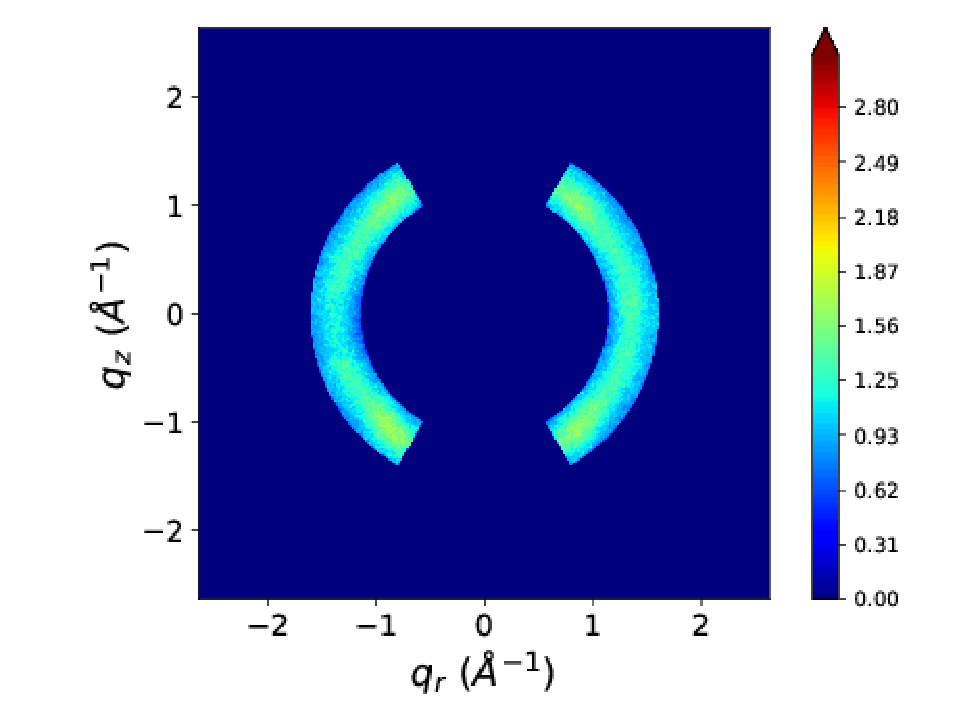
\includegraphics[width=\textwidth]{ralkanes.pdf}  % Search WAXS.py for: fancy demo of r-alkanes normalization
  \caption{R-alkanes}\label{fig:ralkanes}
  \end{subfigure}
  \begin{subfigure}{0.45\linewidth}
  \centering
  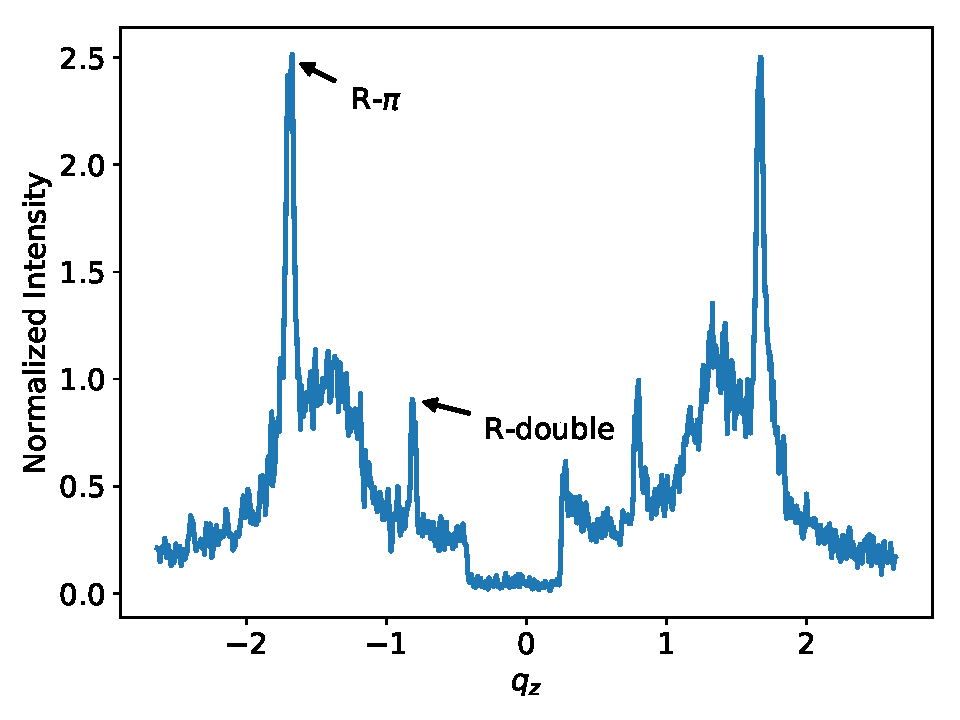
\includegraphics[width=\textwidth]{rpi_rdouble.pdf}  %  Search WAXS.py for: R-pi / R-double intensity measurement illustration
  \caption{$q_z|_{r=0}$}\label{fig:rpi_rdouble}
  \end{subfigure}
  \begin{subfigure}{0.45\linewidth}
  \centering
  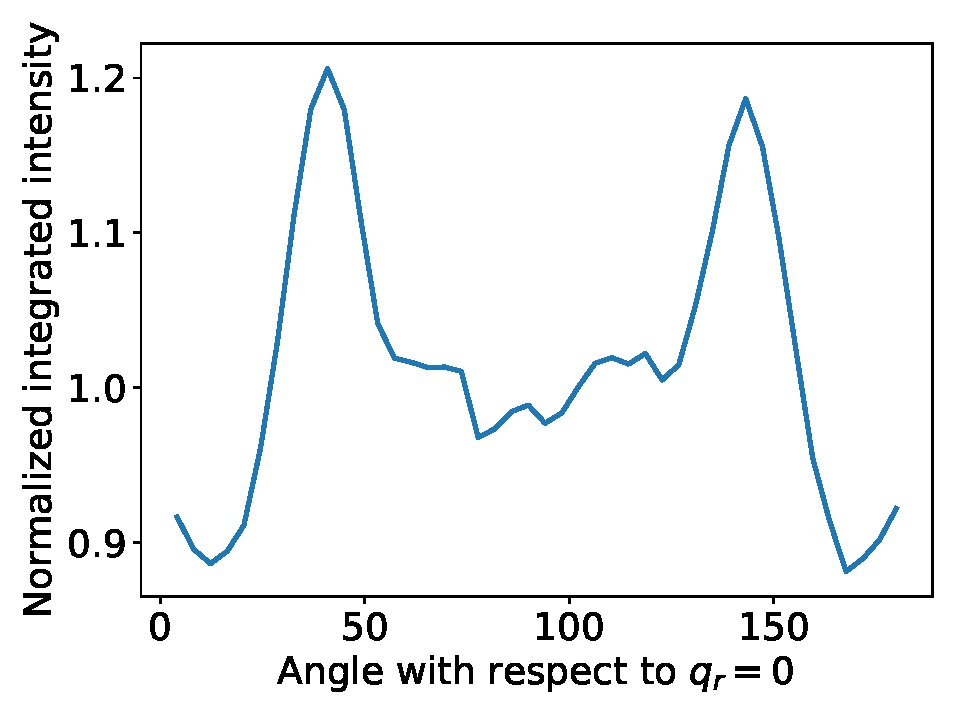
\includegraphics[width=\textwidth]{angular_integration.pdf} % Search WAXS.py for: Plot R-spots integrated intensity curve
  \caption{R-spots}\label{fig:rspots}
  \end{subfigure}
  \begin{subfigure}{0.45\linewidth}
  \centering
  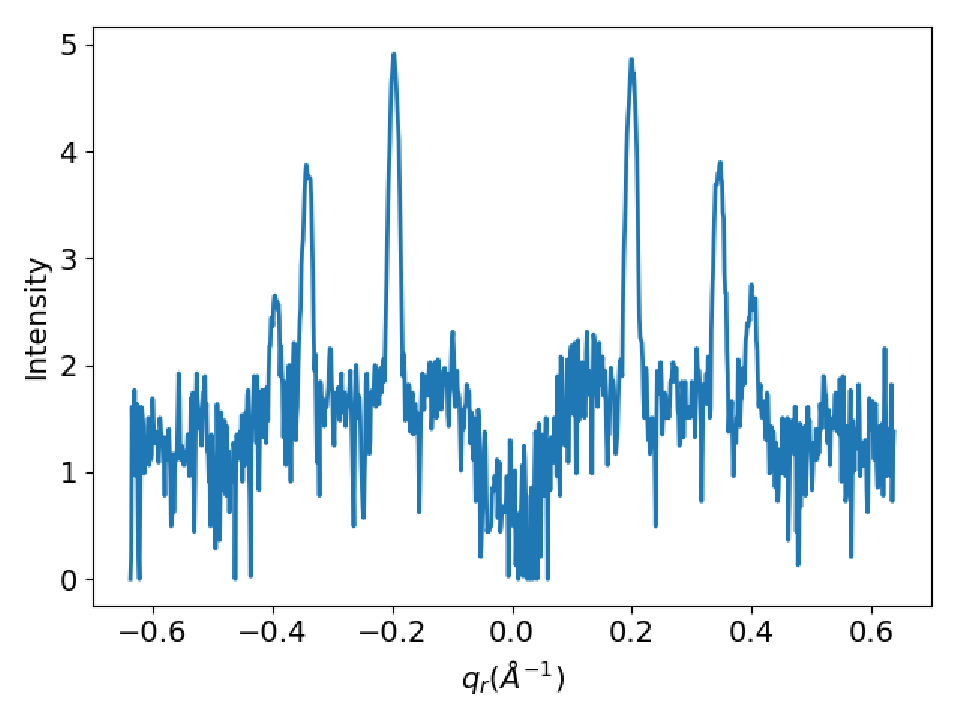
\includegraphics[width=\textwidth]{saxs_xsection.pdf}  % 2DSAXS.py in Scripts folder 
  \caption{R-pores}\label{fig:saxs_xsection}
  \end{subfigure}
  \caption{(a) We measured the intensity of R-alkanes by calculating the average 
  intensity within the region bounded by $|\mathbf{q}|$ = 1.4~$\AA^{-1}$ and 
  1.57~$\AA^{-1}$ (between 4.0 and 4.5 \AA~in real space). We excluded intensities
  within $\pm$ 30\degree~of the meridional axis defined by $q_r=0$, since the 
  simulated spectra overlap with R-$\pi$ in those regions in all cases. (b) We
  measured the intensity of R-$\pi$ and R-double based on the peaks of the $q_z$
  cross-section of the diffraction pattern. (c) We measured the intensity of R-spots
  by averaging the peak heights produced by radially integrating the patterns within 
  the R-alkanes region. We took the intensity of R-spots as the average of the 
  peak intensities near 37 and 143$\degree$. (d) We measured the intensity of 
  R-pores by measuring the height of the d\textsubscript{100} peak (the leading
  peak closest to $q_r$=0) of the cross-section of the diffraction patterns along
  the $q_r$ axis at $q_z$=0.} \label{fig:xrd_intensities}
  \end{figure}
 
  \subsubsection{\textit{Pair distribution functions and correlation length}}\label{section:correlation_length}

  The normalized pair distribution function, $g(\mathbf{r})$, describes
  the probability of finding a pair of particles separated by $\mathbf{r}$,
  \begin{equation}
	g(\mathbf{r})= \frac{1}{\rho N} \Bigg \langle \sum_{i=1}^{N}\sum_{j\neq i}^{N} \delta(\mathbf{r}+\mathbf{r_j}-\mathbf{r_i}) \Bigg \rangle
	\label{eqn:correlation}
  \end{equation}
  where $\rho$ is the average number density of particles and
  $\delta(\mathbf{r})$ is the Dirac delta function\cite{kuriabova_linear_2010}.
  We applied Equation \ref{eqn:correlation} in three dimensions and then
  extracted one dimensional distribution functions using slices of the grid
  along the appropriate axis.

  We measured the one dimensional pair distribution function, $g(z)$, between centers 
  of masses (COMs) of aromatic head group rings along the $z$-axis (perpendicular to
  the membrane plane). We averaged all 1D $z$-directional slices of the full 3D 
  correlation function within 2.1~\AA~of $(x, y)=(0, 0)$. We chose 2.1 \AA~as a crude 
  approximation of the radius of the phenyl ring plane. 
  We calculated the radius as the sum of the longest C-C distance within a phenyl 
  ring (2.8~\AA) and two times the carbon atom electronic radius (0.7~\AA)~\cite{slater_atomic_1964}.
  In this study, $g(z)$ is characterized by an oscillatory function with a period equal to the
  average distance between stacked monomers, and an amplitude that decays exponentially
  (see Figure~\ref{fig:correlation}). The rate of decay is related to the correlation 
  length, L, between monomer head groups. We estimated L by fitting the peaks of $g(z)$,
  using the python package \texttt{scipy.optimize.curve\_fit}~\cite{oliphant_python_2007},
  to a decaying exponential function of the form:
  \begin{equation}
  	Ae^{-z/L}
  	\label{eqn:decaying_exponential}
  \end{equation}
  where A is a fitting parameter for amplitude, $z$ is the independent variable of $g(z)$, 
  and L is the fit correlation length. We calculated the error in the estimated value
  of L as the square root of the diagonal entry of the covariance matrix of 
  optimized fit parameters.
  
  We also used $g(z)$ to calculate the equilibrated vertical stacking distance between
  monomers, $d_{equil}$. We fit a decaying sinusoidal function (using \texttt{scipy.optimize.curve\_fit}) to 
  $g(z)$ of the form:
  \begin{equation}
  	1 - A\cos\left(\frac{2\pi}{\mathit{d}_{equil}}z + B\right)e^{-z/L}
  	\label{eqn:decaying_sinusoid}
  \end{equation}
  where A and B are fit parameters for the function's amplitude and phase shift respectively.
  This function could be used in place of Equation~\ref{eqn:decaying_exponential}, however
  it does not consistently fit the peaks of $g(z)$ from parallel displaced configurations 
  well enough to extract a reliable value of L.
  
  \subsubsection{\textit{Radial distribution functions}}\label{method:rdfs}

  We explored the pores' compositions by measuring the average number densities
  of various monomer components as a function of distance from the pore centers.
  We looked at the average number density of sodium ions, aromatic rings and 
  carbon atoms making up the monomer tails. We binned the radial distance of all
  atoms in each group from the pore centers, then normalized by the volume of the
  annulus defined by the bin edges and the z box vector (See Figure \ref{S-fig:rdf_diagram}
  of the SI). 

  \subsection{Simplified Systems}\label{method:simple_systems}
  
  In order to gain a deeper understanding of discrepancies between the
  experimental and simulated R-$\pi$ reflection, we used a simplified model where
  we represent each monomer as a single point scatterer located at the COM of its
  head group. In order to make a system approximately similar to our equilibrated
  simulation geometries, we created 4 hexagonally packed pore regions spaced 42.5
  \AA~ apart, each with 5 columns of scatterers spaced 4.4 \AA~apart in the
  $z$-direction. We built the system 4 times taller in the $z$-direction (80
  scatterers per column) in order to access higher $q_z$ resolution.
  
  We gave the simplified models the same amount of disorder present in the
  atomistic simulations. We observe two sources of disorder in our atomistic
  simulations: thermal motion of atoms during the simulation and quenched
  disorder created by rapid structural rearrangement during early equilibration
  that is largely locked into place for the remainder of the simulation, even at
  the 100 ns time scale. We measured thermal disorder by calculating the standard
  deviation of the distribution of head group COM positions from their average
  positions. We measured quenched disorder by calculating the standard deviation
  of the distribution of head group COMs from their idealized average positions.
  In the $z$-direction, we measured the deviation of the head group COMs from an
  equally spaced column of head groups. In the $xy$ plane, we calculated the
  standard deviation in radial position from the pore center and the angular
  deviation from equally spaced points surrounding the pore center. This method
  for calculating quenched disorder inherently includes the convoluted thermal
  disorder. 
  
  We approximated interactions between particles by correlating the $z$-distance 
  between points within each column of point scatterers. We placed points in each
  column by drawing random samples from a multivariate normal distribution defined
  by the mean positions of an equally spaced column of points. We gave the 
  distribution at each point along the column the same standard deviation, 
  $\sigma_z$, and we defined a covariance matrix such that the covariance, $v$, of
  the distance, $d$, between scatterers decays exponentially from $v$ according
  to the equation $ve^{-d/L}$, where $L$ is the correlation length. Unless noted
  otherwise, we used the experimental correlation length of 9.0 \AA. 
  
  We calculated averaged R-$\pi$ profiles by simulating the diffraction pattern
  of trajectories consisting of 1000 independent simple system configurations 
  generated with point scatterer placement based on the quenched disorder seen in
  atomistic simulations. The quenched disorder observed in the atomistic simulations
  is up to 8 times greater in magnitude than thermal disorder (See Table~\ref{table:quenched_disorder}
  in Section~\ref{section:rpi}). This method for simulating time-averaged R-$\pi$ profiles
  assumes that the timescales for large scale rearrangements of the
  system are much longer than what we can feasibly simulate with MD.

  \subsection{\textit{Ionic conductivity calculations}}\label{method:ionic_conductivity}

  We calculated ionic conductivity using the Nernst-Einstein relationship, which 
  relates the DC ionic conductivity, $\sigma$, to ion diffusivity, $D$, 
  concentration, $C$, ion charge, $q$, the Boltzmann constant, $k_b$, and 
  absolute temperature, $T$: 
  \begin{equation}
	\sigma = \dfrac{q^2CD}{k_b T} 
	\label{eqn:nernst_einstein}
  \end{equation}
  We measured sodium ion diffusion coefficients by calculating the slope
  of the linear region of the $z$-direction mean square displacement curve as
  indicated by the Einstein relation \cite{einstein_investigations_1956}. We
  visualized the MSD plot to determine where to begin and end a linear fit. We
  measured ion concentration with respect to the volume of the entire unit cell. 
  More details are provided in the SI, Section \ref{S-section:ionic_conductivity}.

  \subsection{Cross-linking}\label{method:xlink}
  
  In order to better match the experimental membrane synthesis process,
  we created a cross-linking algorithm that one can apply to equilibrated structures. 
  The primary purpose of cross-linking experimentally is to create a mechanically robust membrane.
  For that reason, we are not concerned with replicating the kinetics of the reaction, 
  but instead emphasize understanding how much and in what way cross-linking modulates
  the system's structure.

  We based our cross-linking algorithm on the known reaction mechanism 
  (Figure \ref{S-fig:xlink_mech} of the SI). The reaction 
  takes place at the terminal vinyl groups
  on each alkane tail. The procedure is carried out iteratively. Each iteration, the
  algorithm chooses carbons to cross-link based on the distance between eligible 
  carbon pairs. The algorithm then updates the topology with the new bonds and atom
  types, energy minimizes the system and runs a short simulation before selecting 
  the next group of eligible carbons atoms.
  
  \section{Results and Discussion}
  
  \subsection{Density of monomers around pores}\label{section:mon_per_pore}
  
  Our simulations best support a model built with 5 monomer columns per pore
  based on the measured equilibrated pore-to-pore distances. To identify the
  density of monomer columns around each pore, addressing Question
  \ref{point:monomernum} in the introduction, we ran simulations of systems
  created with 4--8 columns per pore. We built systems in both the parallel
  displaced and sandwiched configurations and equilibrated them according to the
  dry equilibration procedure. We tested all systems with an initial vertical
  monomer spacing, $\mathit{d}$, of 3.7 \AA~in accordance with R-$\pi$. We tested
  4 additional systems with monomers initially spaced 5 \AA~apart vertically (see
  Section \ref{S-section:initial_pore_spacing} of the SI for more details on
  sensitivity to initial monomer spacing). We considered the pore-to-pore
  spacing to be equilibrated as defined in Section~\ref{method:equil_time}.
  Figure~\ref{fig:p2p} shows the equilibrated pore-to-pore distances for all
  systems tested. 
  
  \begin{figure}[!htb]
	\centering
	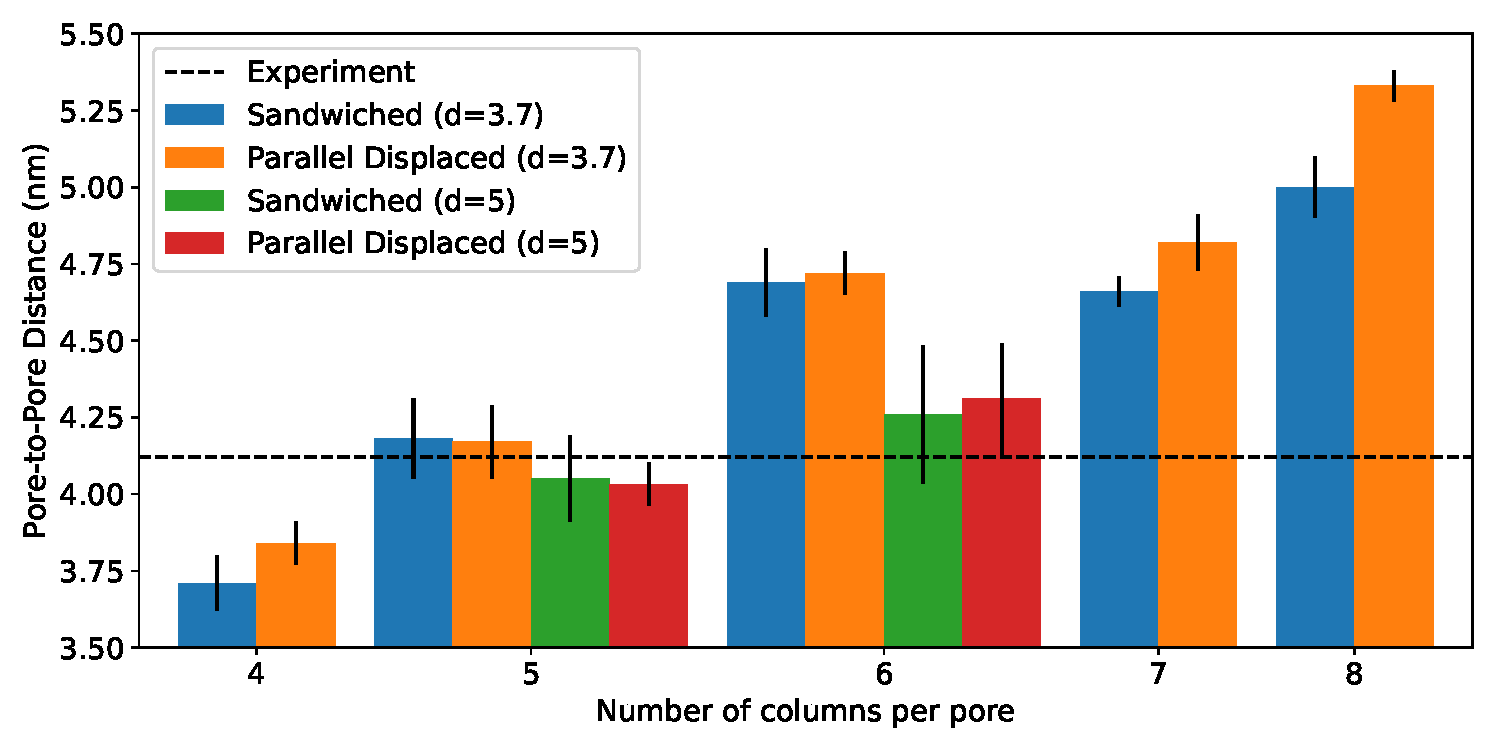
\includegraphics[width=\linewidth]{p2p.pdf}
	\caption{Systems with 5 columns per pore have equilibrated pore spacings closest to
			 the experimental value of 4.12 nm. The equilibrated pore spacing of the model 	
			 increases as the number of columns in each pore increases.}~\label{fig:p2p}
  \end{figure}  
  
  All systems tested, although equilibrated from the perspective of the metrics
  used here, are frozen in metastable basins. Not all make physical sense or fit
  the experimental profile that we are trying to match. In the limit of infinite
  simulation time, all systems will in theory converge to a single equilibrium
  configuration, but that time is far beyond the 100's of nanoseconds simulated
  here. For simplicity, we group the systems studied here into the ordered and
  disordered basins. What we find is that any system equilibrated with
  $\mathit{d}=3.7$ \AA~can generally be characterized as being in a more ordered
  basin, and any system equilibrated with $\mathit{d}=5.0$ \AA~can be
  characterized as being in a more disordered basin. The extra space between
  stacked monomers in the disordered basin systems gives the monomer head groups
  more rotational freedom. We quantified the ordering of the head groups using
  the nematic order parameter (see Section \ref{S-method:nematic_order} for
  details of the calculation). Disordered basin systems have a lower nematic
  order parameter (meaning they are more disordered) than ordered basin systems.
  Generally, when monomers are started further apart, they stay further apart
  than systems where monomers are started closer together (see
  Table~\ref{table:correlation_length}). This increased equilibrated stacking
  distance of monomers in disordered basin systems increases their discrepancy
  with experimental stacking distances derived from WAXS relative to ordered
  basin systems (See Section~\ref{section:rpi}). 
  
  Systems built with 5 columns around each pore equilibrate to a pore spacing
  that is most consistent with the experimental value of 4.12 nm derived from
  SAXS measurements (Figure~\ref{fig:SAXS}). Ordered basin systems built with 4
  columns per pore equilibrate to an average pore spacing 0.25 nm lower than
  experiment. Ordered basin systems built with 6 columns per pore, have an
  equilibrated pore spacing ca. 0.50 nm higher than experiment. Monomers in
  disordered basin systems built with 6 columns-per-pore agree with experimental
  pore-to-pore distances within error, but stack too far apart. 6
  column per pore disordered sandwiched and disordered parallel displaced
  configurations stack $\sim$~4.87 and 4.94 \AA~apart respectively, which is
  $\sim$ 1.2~\AA~further apart than suggested by experiment. 5 column-per-pore
  systems stack, at a maximum, 0.9 \AA~further apart than experiment (see
  Table~\ref{table:correlation_length}). The remainder of this discussion will
  therefore focus on the analysis of systems built with 5 columns per pore. 

  \subsection{Simulated XRD comparison to 2D-WAXS data}

  We can better understand the structure of the system by simulating XRD
  patterns produced from equilibrated MD trajectories (see
  Section~\ref{method:xrd}) and comparing these simulated patterns to experiment,
  addressing Question~\ref{point:xrdmatch} in the Introduction. We tested systems
  built with 5 columns per pore in the parallel displaced and sandwiched
  configurations at 300 K in the ordered and disordered basins, as those were the
  most consistent with the most unambiguous XRD features, the pore-to-pore
  spacing and the stacking distance, as described in
  Section~\ref{section:mon_per_pore}.  We generated simulated patterns using the
  locally equilibrated portion of each simulation trajectory (see
  Section~\ref{method:equil_time}). There are two important factors to take into
  account when looking at differences between experimental and simulated XRD
  patterns.  First, the simulated diffraction patterns have some noise,
  especially along the $q_z$ axis at $q_r$=0, which is where several of the more
  interesting features are located. This is due to the angle averaging of the 3D
  structure factor around the $q_z$-axis, meaning there are fewer samples as
  $q_r$ approaches 0.  More importantly, our simulations do not appear to be long
  enough to sample truly independent configurations within their respective
  metastable basins (see Section~\ref{section:slow_dynamics}), meaning we must
  take care in interpreting the results of the XRD. The amount of independent
  configurations required to converge along the $q_z$ axis is analyzed in SI,
  Section \ref{S-section:xrd_noise}. The simulated patterns generated for all
  systems studied are shown and compared to experiment in
  Figure~\ref{fig:XRDsim}.

  \begin{figure}[!htb]
	\centering
	\begin{subfigure}{0.905\textwidth}
	\begin{subfigure}{0.28\linewidth}
			\begin{subfigure}{\textwidth}
			\centering
		        	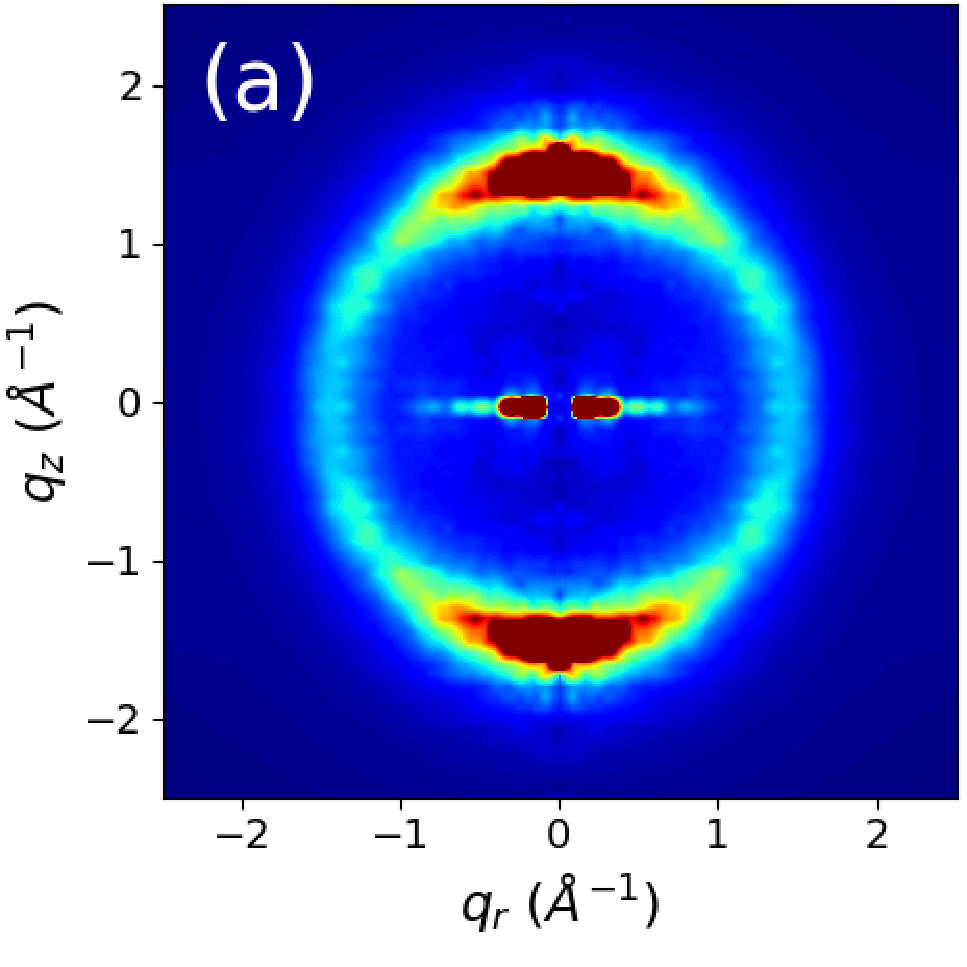
\includegraphics[width=\linewidth]{rzplot_layered_300K_jet_nocbar.pdf}
			\end{subfigure}
			\begin{subfigure}{\textwidth}
		       		\centering
	        		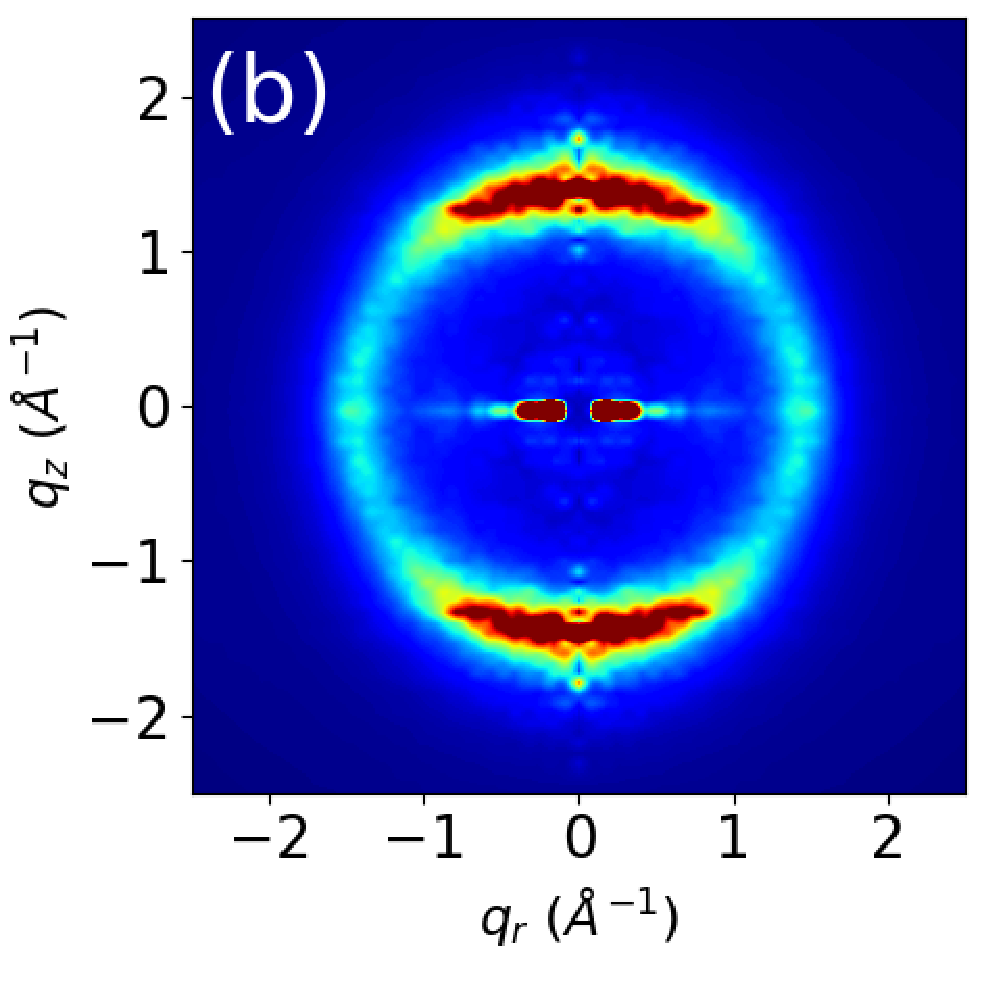
\includegraphics[width=\linewidth]{rzplot_layered_300K_disorder_jet_nocbar.pdf}
			\end{subfigure}
	\end{subfigure}
	\begin{subfigure}{0.4\linewidth}
	\centering
			\begin{subfigure}{\textwidth}
		       		\centering
	        		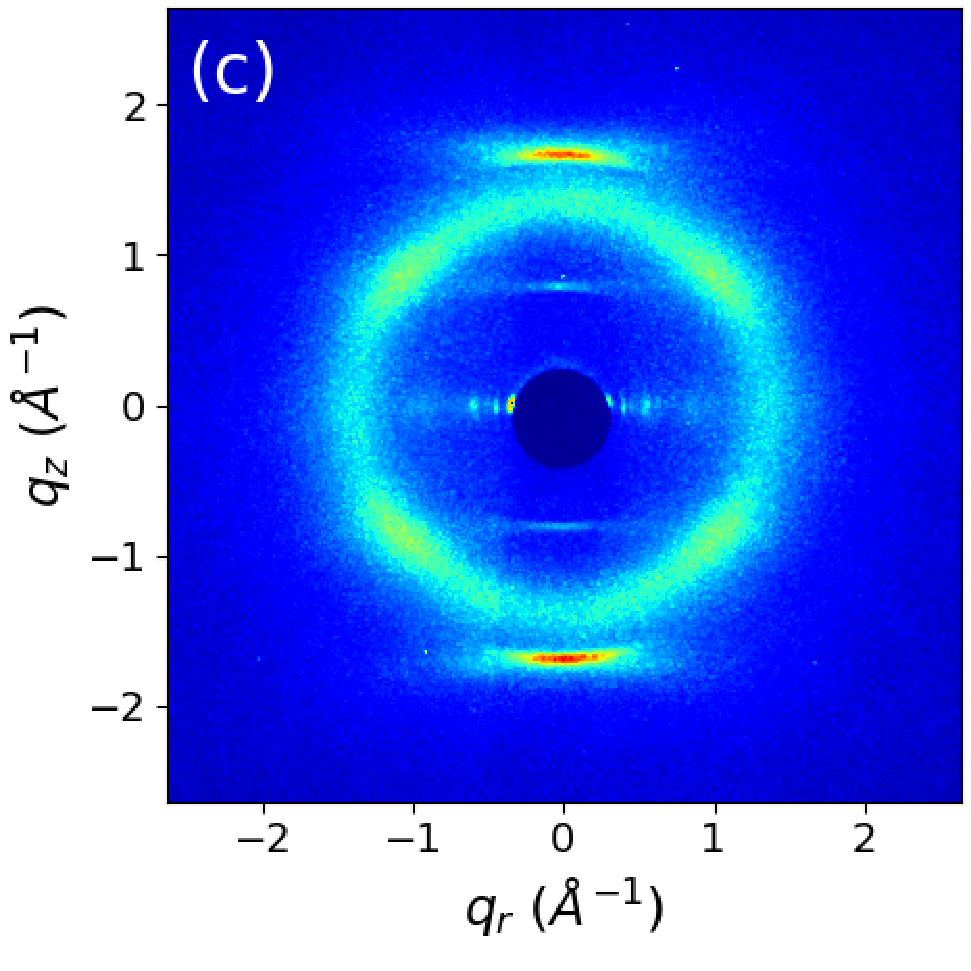
\includegraphics[width=\linewidth]{WAXS_raw_jet_nocbar.pdf}
			\end{subfigure}
	\end{subfigure}
	\begin{subfigure}{0.28\linewidth}
	\centering
			\begin{subfigure}{\textwidth}
			\centering
		        	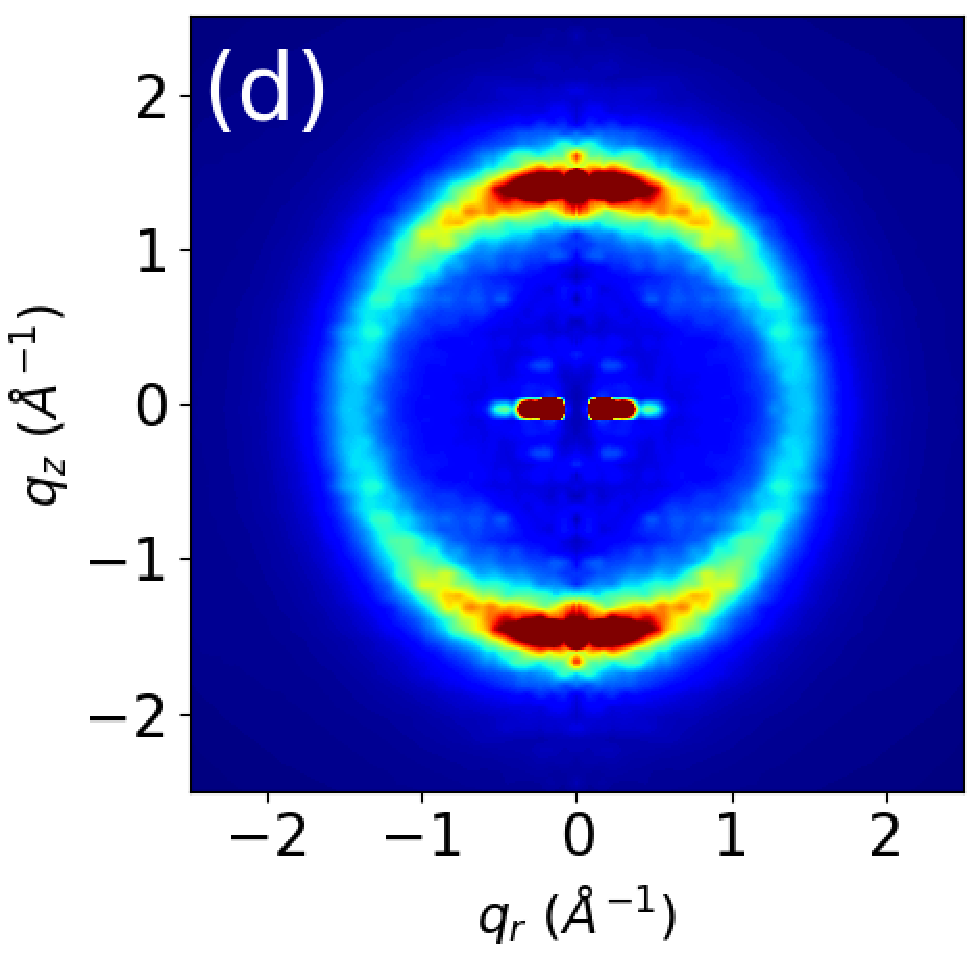
\includegraphics[width=\linewidth]{rzplot_offset_300K_jet_nocbar.pdf}
			\end{subfigure}
			
			\begin{subfigure}{\textwidth}
				\centering
			    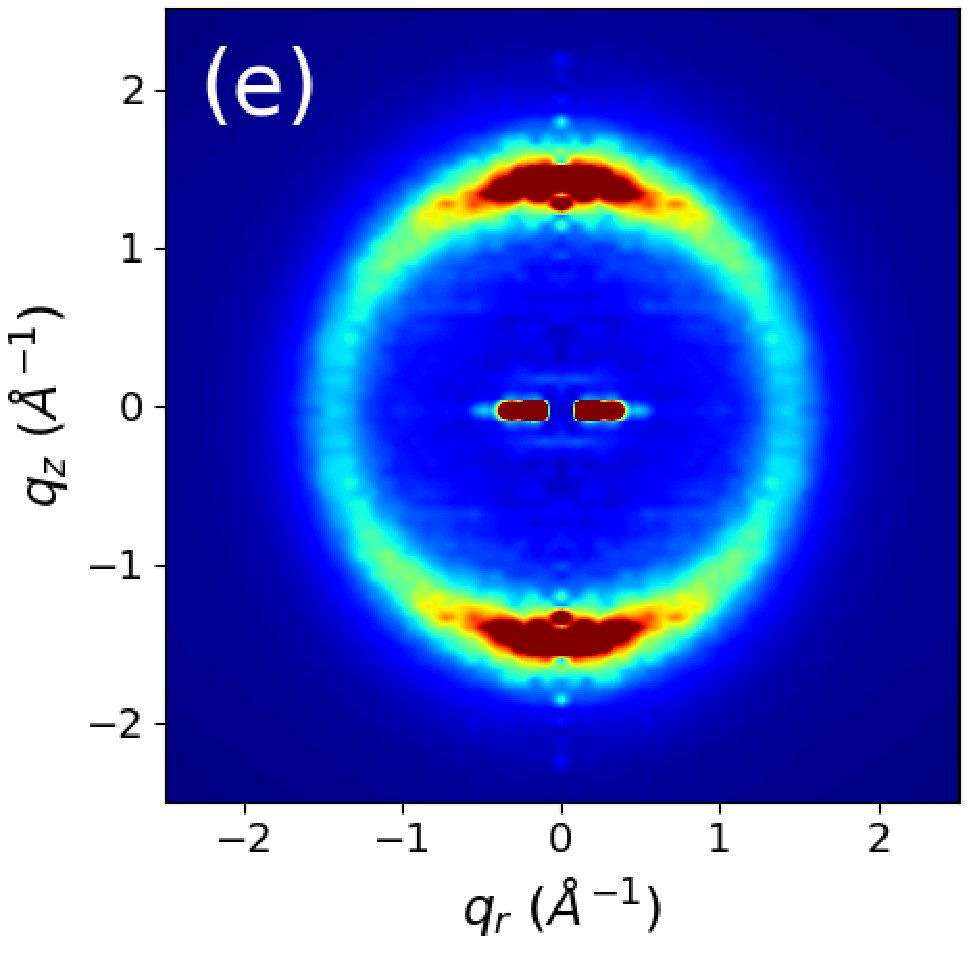
\includegraphics[width=\linewidth]{rzplot_offset_300K_disorder_jet_nocbar.pdf}
			\end{subfigure}
	\end{subfigure}
	\end{subfigure}
	\begin{subfigure}{0.085\textwidth}
		\centering
		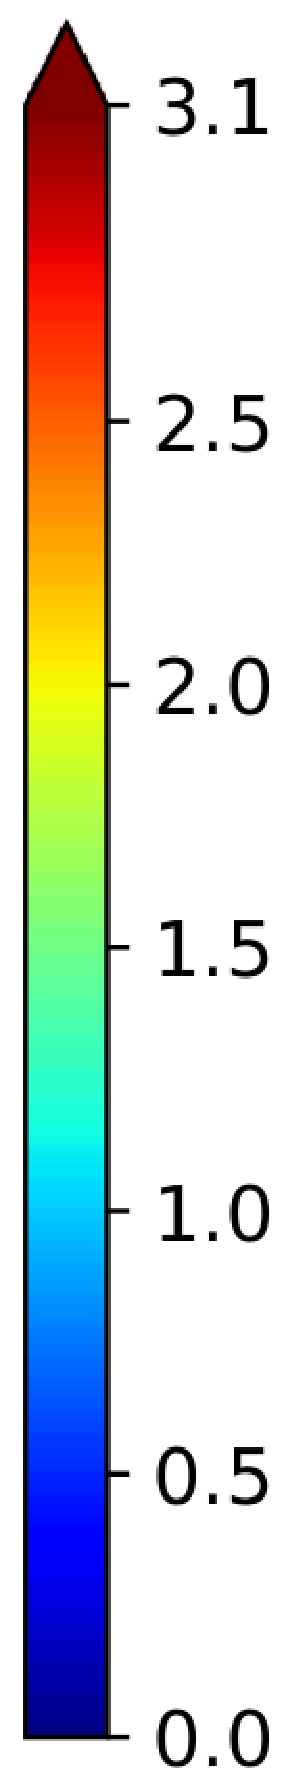
\includegraphics[width=\linewidth]{colorbar_jet.pdf}
	\end{subfigure}	
	\caption{Simulated XRD patterns show some qualitative agreement with
		experiment. Shown is a comparison of the (a) Sandwiched, ordered basin (b)
		Sandwiched, disordered basin (d) Parallel displaced, ordered basin and (e)
		Parallel displaced, disordered basin configurations with (c) experimental WAXS.
		The major reflections of interest (See Figure~\ref{fig:SWAXS} for their
		definitions) are present at varying degrees. In all cases, R-pores, R-alkanes
		and R-$\pi$ are present to some degree. R-spots is also present, however it is
		generally partially covered by the broad R-$\pi$ reflection. Quantitative
		comparisons of the relative intensities and locations of reflections of
		interest are presented in Table~\ref{table:relative_intensities_300K}. In both
		XRD patterns generated from parallel displaced configurations, there is a faint line
		across $q_z \sim 0.7~$\AA$^{-1}$, half the simulated value of R-$\pi$. Although
		it does not cross through $q_r = 0$~\AA$^{-1}$, it is at the same $q_z$ value
		where we expect R-double to be present. Still, R-double is not fully reproduced
		in any of the simulated patterns.}~\label{fig:XRDsim} 
  \end{figure}
  
  The simulated XRD patterns show moderate agreement with experiment. There 
  are key qualitative and quantitative differences between the experimental and simulated
  locations and intensities of each major reflection. The integrated intensity and location
  of each simulated reflection relative to its experimental counterpart are shown in  
  Table~\ref{table:relative_intensities_300K}. Our approach for measuring the intensity of
  each reflection is described in Section~\ref{method:xrd}. 

  In the next few subsections, we individually address each major reflection, and the
  similarities and differences between simulation and experiment. We start with relatively 
  uncomplicated analyses of reflections that are very similar between experiment and simulation:
  \begin{itemize}
  	\item The location of R-alkanes (Section~\ref{section:ralkanes})
  	\item The location and intensity of R-pores (Section~\ref{section:rpores})
  \end{itemize}
  and then move onto more complicated explanations of those reflections whose characteristics
  do not match, or have not been fully explained by experiment:
  \begin{itemize}
  	\item The origin of R-spots (Section~\ref{section:rspots})
  	\item The position, shape and intensity of R-$\pi$ (Section~\ref{section:rpi})
  	\item The origin of R-double (Section~\ref{section:rdouble})
  \end{itemize}
  
\begin{table}[h]
  \centering
  \begin{tabular}{c|ccccc}
  \toprule
 		     & \multicolumn{5}{c}{Normalized Reflection Intensity}                   \\
  \hline
             &            &            & Parallel  & Disordered & Disordered         \\
  Reflection & Experiment & Sandwiched & Displaced & Sandwiched & Parallel Displaced \\
  \midrule
  R-alkanes  & 1.0        &  1.0       &  1.0      &  1.0       &  1.0               \\
  R-pores    & 4.91       & 49.5       & 54.0      & 50.8       & 53.4               \\
  R-spots    & 1.2        &  1.2       &  1.2      &  1.1       &  1.1               \\
  R-$\pi$    & 2.8        & 44.0       &  7.7      &  8.4       & 10.1               \\
  R-double   & 0.9        &  --        & --        &  --        & --                 \\ 
  \hline
   		     & \multicolumn{5}{c}{Reflection Location ($|\mathbf{q}|~\AA^{-1}$)}     \\
  \hline
             &            &            & Parallel  & Disordered & Disordered         \\
  Reflection & Experiment & Sandwiched & Displaced & Sandwiched & Parallel Displaced \\
  \midrule
  R-alkanes  & 1.39       &  1.44      &  1.44     & 1.42       & 1.43               \\  
  R-pores    & 0.176      &  0.170     &  0.170    & 0.173      & 0.172              \\
  R-spots    & 1.39       &  1.44      &  1.44     & 1.42       & 1.43               \\
  R-$\pi$    & 1.70       &  1.41      &  1.42     & 1.40       & 1.40               \\
  R-double   & 0.85       &  --        & --        &  --        & --                 \\ 
  \bottomrule
  \end{tabular}
    \caption{The simulated XRD patterns of the systems tested, normalized so that
	  the average intensity of R-alkanes in each pattern equals 1, show R-pores and
	  R-$\pi$ reflections that are significantly higher than experiment and R-spots
	  reflections that are slightly lower than experiment. R-double does not appear
	  in any simulated patterns, and thus has no measurable intensity. In terms of 
	  the locations of the reflections, R-pores, R-alkanes and R-spots appear at $|\mathbf{q}|$
	  values that are close to experiment, while R-$\pi$ appears at a significantly lower
	  $|\mathbf{q}|$ value than experiment.\label{table:relative_intensities_300K}}
  \end{table}  
  
  \subsubsection{The location of R-alkanes}\label{section:ralkanes}

  We normalized the experimental and simulated diffraction patterns so that the
  average intensity within R-alkanes is equal to 1 because we believe that
  R-alkanes is the experimental feature most likely to be reproduced by our
  simulations. We reached this conclusion because alkane parameters in GAFF and
  AMBER forcefields generally reproduce data
  well.~\cite{wang_development_2004,caleman_force_2012} 

  R-alkanes appears close to its expected location. In all cases, the maximum
  intensity of R-alkanes along the $q_r$ axis at $q_z$=0, which we use to
  estimate its location, appears at a $|\mathbf{q}|$ value that is, at most,
  3.5\% higher than experiment. The error in the simulated diffraction patterns
  is less than the error due binning in each frequency direction, so was not
  further investigated. 

  \subsubsection{The location and intensity of R-pores}\label{section:rpores}
  
  R-pores is about 10 times more intense than experiment in all simulated
  systems. Some or all of this discrepancy may be a consequence of our
  normalization of the experimental 2D-SAXS pattern, since the common peak
  between it and the 2D-WAXS patterns is partially obscured by the beamstop in
  the WAXS. If our simulations do indeed predict an intensity of R-pores that is
  too high, we hypothesize that this is primarily due to the relatively perfect
  infinite hexagonal array of pores in the simulated systems. In the real system,
  periodicity of the hexagonal array is disrupted by misalignment of the
  crystalline domains and the pore-to-pore distances fluctuate more over long
  time scales. The agreement in intensity in R-pores obtained here is sufficient for this
  study because this intensity is primarily controlled by longer-range
  organization that cannot be captured by simulation of only 4 pores and because
  we are only concerned with the structure of the individual pores themselves. 
  
  The location of the leading peak of R-pores is directly related to the
  average distance between pores. However, there is substantial uncertainty in
  the exact location relative to the bin size resulting from the Fourier space
  transformation. We can instead measure the average distance between columns
  with more precision in real space (See Section~\ref{method:pore_spacing}). We
  showed that we achieve experimentally consistent pore spacings in our
  simulations in Section~\ref{section:mon_per_pore}. 

  \subsubsection{The origin of R-spots}\label{section:rspots}
  
  The intensity of R-spots is close to experiment when generated from any of
  our simulated systems. We measured its intensity as outlined in Section~\ref{method:xrd}.

  In order to more clearly identify the structural reasons for R-spots, we
  equilibrated an ordered basin sandwiched configuration at 280 K to moderately
  increase the order and therefore intensity. Many force fields do not obtain
  the correct equilibrium structure at precisely the experimental temperature.
  Wang et al. highlighted the shortcoming of some of the most popular protein
  force fields in predicting the temperature dependence of protein structural
  ensembles \cite{wang_building_2017}. It is therefore possible that   % page 12
  our membrane system, simulated at 300 K, is under-structured in the tail region
  compared to the experimental structure at 300 K. We found that lowering the
  temperature indeed better resolved R-spots (Figure~\ref{fig:sandwiched280K}),
  suggesting that our `effective' temperature might indeed be too high,
  understabilizing structure. 

  Previous literature has attributed the R-spots reflection in this particular
  WAXS dataset as the result of tilted alkane chains~\cite{feng_scalable_2014}.
  We measured the tilt angle of the alkane chains of the 280 K system by measuring
  the angle made by the vector extending from top to bottom of each tail with
  respect to the membrane plane. We found that it equilibrates to an average tilt
  angle of -2 $\pm$ 13\degree~(Figure~\ref{fig:tilt}), far from the 37\degree~tilt angle
  previously used to explain R-spots. Even when we placed position restraints on
  the monomers in a tilted initial configuration, monomers quickly reduced their
  tilt relative to the $xy$ plane to an angle statisically indistinguishable from
  zero (see Section \ref{S-section:tail_tilt} of the SI). 

  The evidence from simulations strongly suggest that the source of the R-spots
  reflection is packing of the tails in a hexagonal array.  First, we demonstrate
  R-spots comes primarily from the tails, by removing all non-tail atoms from the
  trajectory and simulating the XRD pattern with the remaining atoms, which
  preserves R-spots (Figure~\ref{fig:tails_rzplot}).  Next, we plotted the center
  of masses of the first four tail atoms of all tails (Figure
  \ref{fig:centroids}). We measured the angle between each COM and its nearest
  neighbor COMs with respect to the $xy$ plane of the membrane. We see distinct
  peaks in the distribution of these angles located ca. $-60\degree$, $0\degree$,
  and $60\degree$, which is consistent with a hexagonally-packed configuration
  (Figure~\ref{fig:layered_tails}).  This ordering is primarily in the parts of
  the tail proximal to the heads, and dies off at the tail ends, where there is
  more space to fill causing them to pack nearly isotropically. See Section
  \ref{S-section:tail_packing} of the SI for a more detailed explanation of the
  calculation and packing distributions generated from different sections of the
  tails.

  The peaks in the nearest neighbor angle distribution due to the hexagonal
  packing are consistent with the location of R-spots. The 2D-Fourier transform
  of a simple hexagonal array constructed based on the peak angles in
  Figure~\ref{fig:layered_tails} shows reflections in the same locations as
  R-spots, in addition to vertical stacking reflections along the $q_z$ axis that
  would intersect with R-$\pi$ (Figure~\ref{fig:hexagonal_ft}). 

  \begin{figure}[!htb]
  \begin{subfigure}{0.32\linewidth}
  	\centering
  	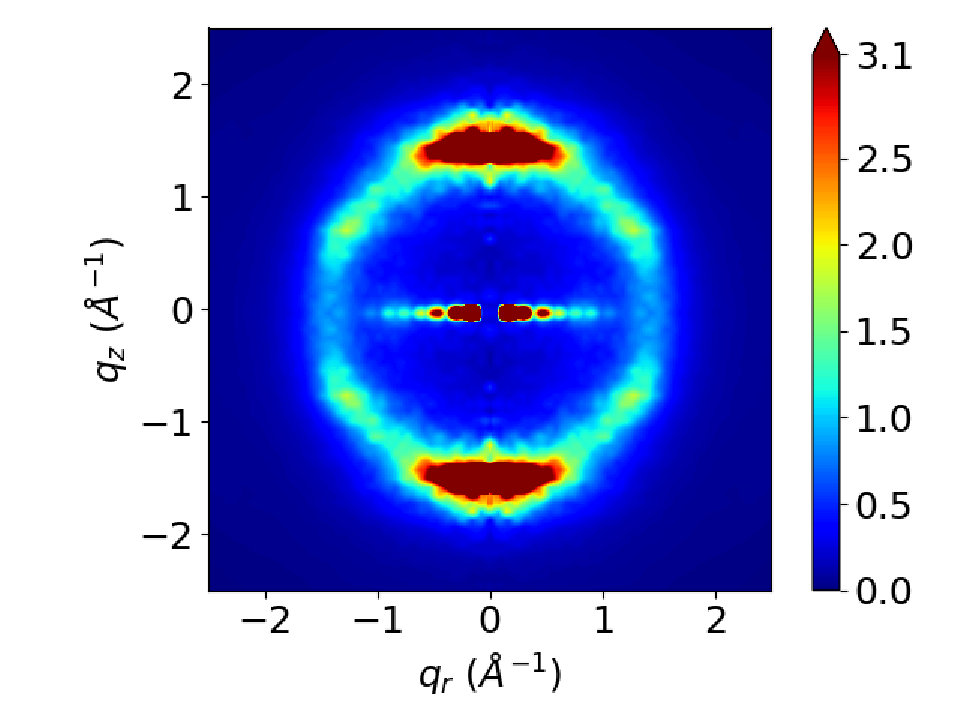
\includegraphics[width=\textwidth]{rzplot_layered_280K_jet.pdf}
  	\caption{}\label{fig:sandwiched280K}
  \end{subfigure}
  \begin{subfigure}{0.32\linewidth}
    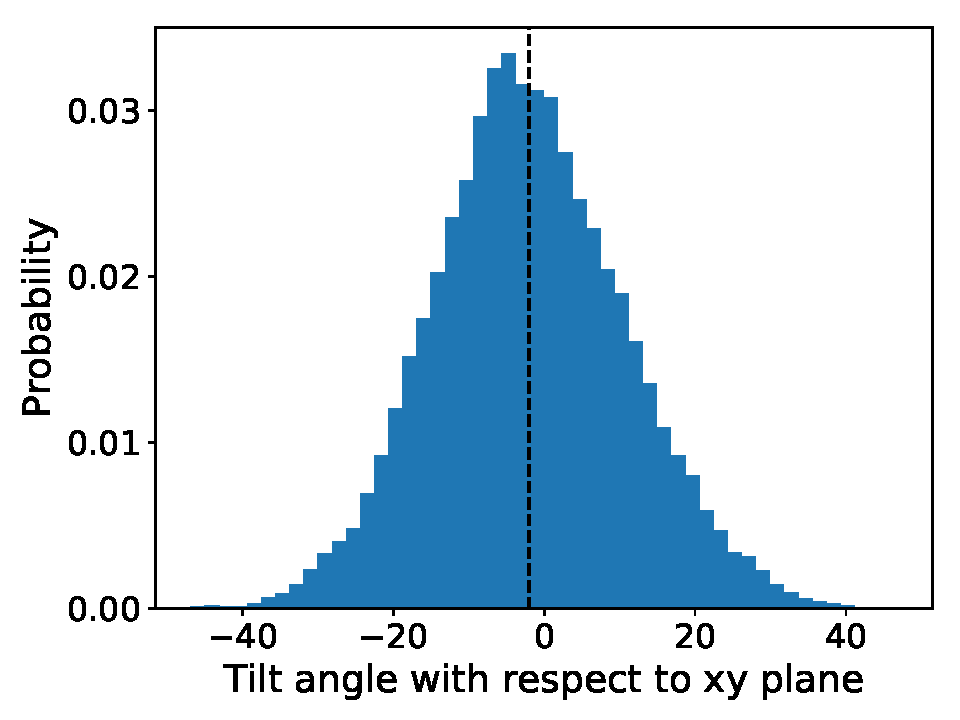
\includegraphics[width=\textwidth]{tilt_dist.pdf}
    \caption{}\label{fig:tilt}
  \end{subfigure}
  \begin{subfigure}{0.32\linewidth}
	\centering
	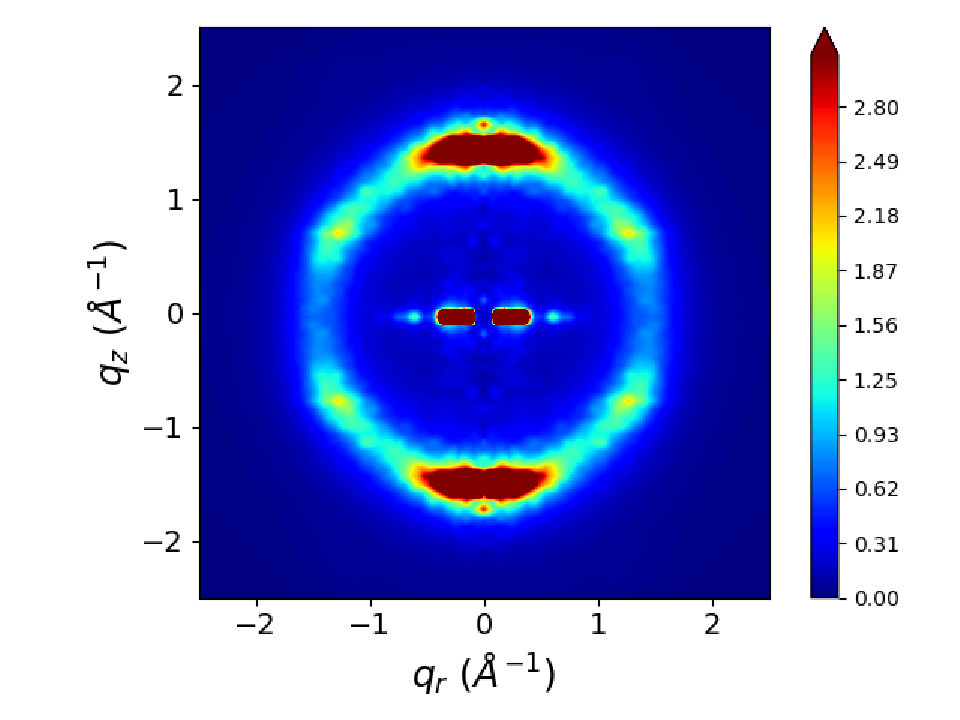
\includegraphics[width=\textwidth]{tails_rzplot_jet.pdf}
	\caption{}\label{fig:tails_rzplot}
  \end{subfigure}
  \begin{subfigure}[t]{0.32\linewidth}
    \centering
	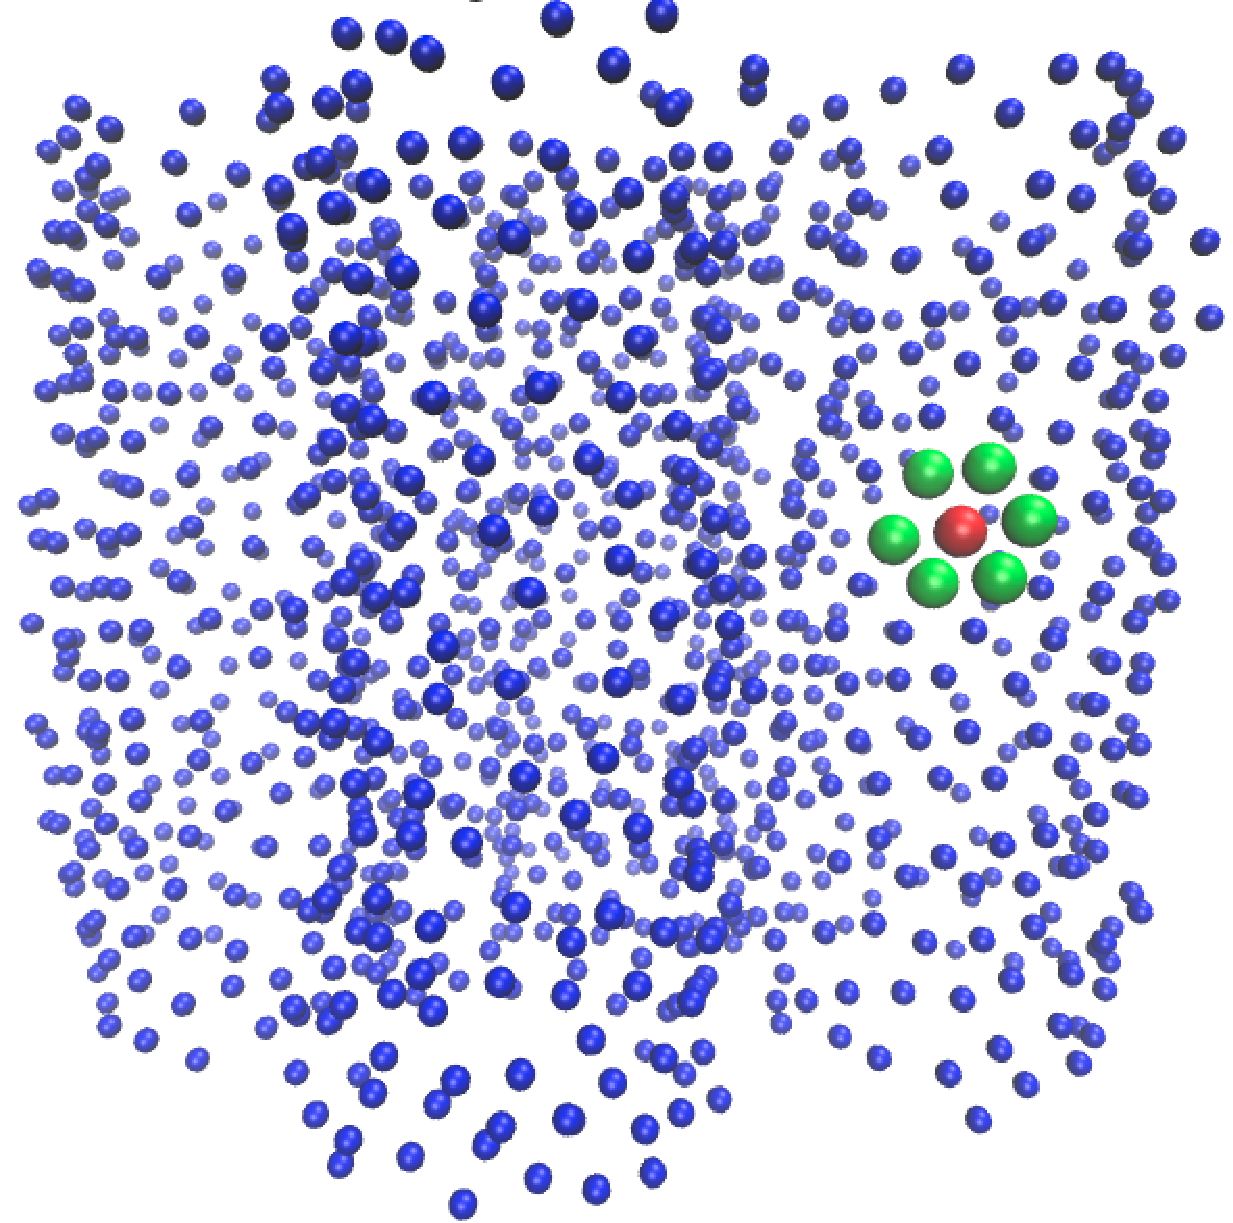
\includegraphics[scale=0.2]{centroids.pdf}
  \caption{}\label{fig:centroids}
  \end{subfigure}
  \begin{subfigure}[t]{0.32\linewidth}
        \centering
	        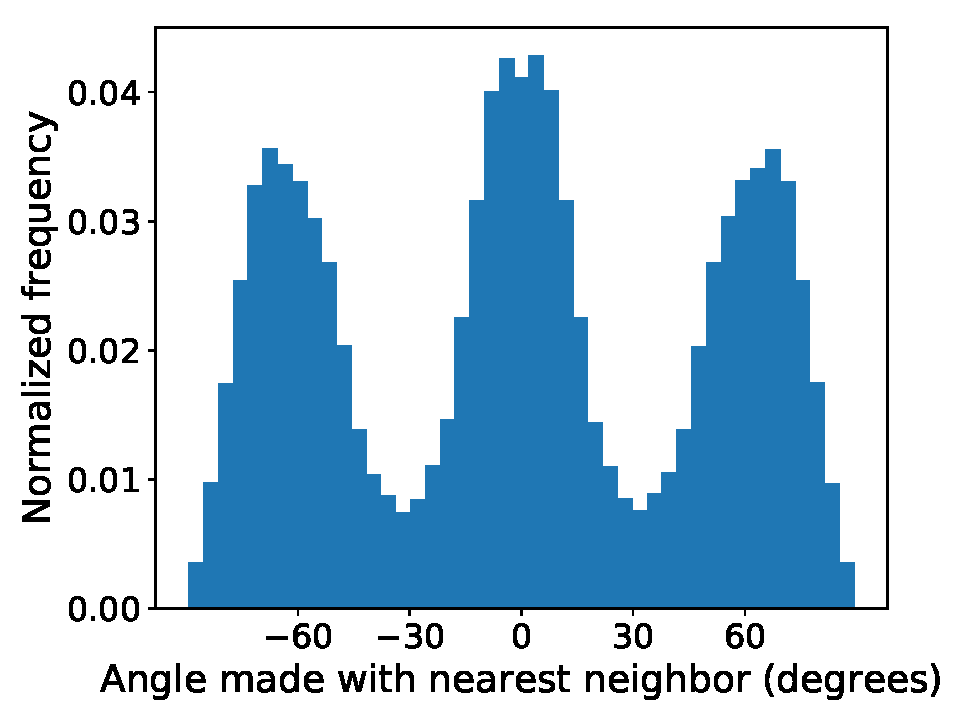
\includegraphics[width=\linewidth]{hexagonal_tail_packing.pdf}
	        \caption{}~\label{fig:layered_tails}
  \end{subfigure}
  \begin{subfigure}[t]{0.32\textwidth}
        	\centering
	        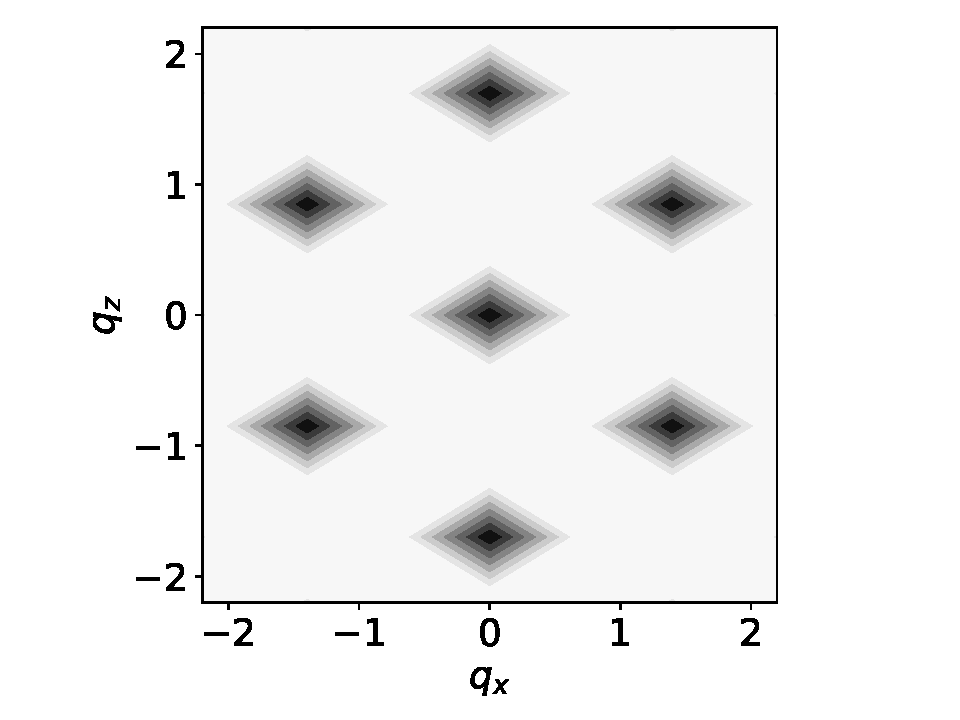
\includegraphics[width=\linewidth]{hexagonal_ft.pdf}  % generated from hexagonal_packing.py
	        \caption{}~\label{fig:hexagonal_ft}
  \end{subfigure}
  \caption{(a) R-spots increases in intensity when the temperature of the system is 
	  lowered to 280 K. (b) We measured the average angle made between each
	  monomer alkane tail and the membrane plane. The average tilt angle (dashed
	  line) is near -2\degree~which is far from the 37\degree~tilt angle previously
	  used to explain R-spots. (c) To isolate the main cause of R-spots, we removed
	  all atoms from the trajectory except for carbon atoms that constitute the
	  tails. The simulated XRD pattern of the tails-only trajectory still shows
	  R-spots. (d) Since the tails stay relatively flat, we plotted the center of
	  mass of the first four carbon atoms of each tail originating from the head
	  groups (for example, green colored centroids in the plot surround the red
	  centroid in hexagonal fashion).  Visually, the packing looks hexagonal. (e) We
	  hypothesize that R-spots is the result of ordered tail packing. Defining the
	  membrane plane to be 0\degree, we measured the angles between each COM and its
	  nearest neighbor COMs for the equilibrated sandwiched configuration simulated
	  at 280 K. Peaks appear in the distribution at $-60\degree$, $0\degree$ and
	  $60\degree$. (f) The Fourier transform of a hexagonally packed grid of points
	  defined by the angles in (e) shows intensity at the same locations where we
	  expect to see R-spots, as well as intensity along the $q_z$ axis
          where R-$\pi$ would appear.}~\label{fig:tail_packing}
  \end{figure}  

  \subsubsection{The position, shape, and intensity of R-$\pi$}\label{section:rpi}

  The position, shape, and intensity of R-$\pi$, generated from simulations at
  300 K have qualitative and quantitative differences from experiment. The
  reflections appear at lower $q_z$ values, they are more intense, and the shape
  of its cross-sections, especially in the $q_r$ direction are different relative
  to the experimental system. For comparison, see
  Figure~\ref{fig:rpi_exp_comparison} where we used cross-sections of the
  simulated XRD generated from the ordered parallel displaced configuration as an
  example. In this section, we explore the various contributions to these
  discrepancies, and use this information to speculate on what reasonable
  differences in the simulations could explain them.
  
  \begin{figure}
  \centering
  \begin{subfigure}{0.45\textwidth}
  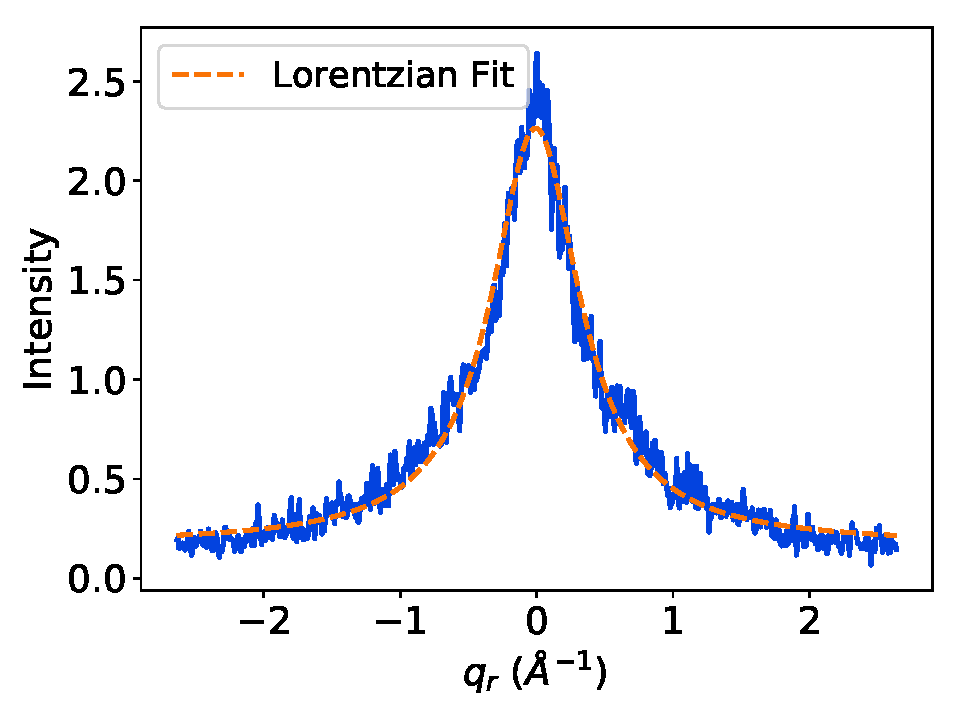
\includegraphics[width=\textwidth]{exp_rsection_fit.pdf}
  \caption{FWHM = 0.792 $\pm$ 0.009 $\AA^{-1}$}\label{fig:exp_rsection_fit}
  \end{subfigure}
  \begin{subfigure}{0.45\textwidth}
  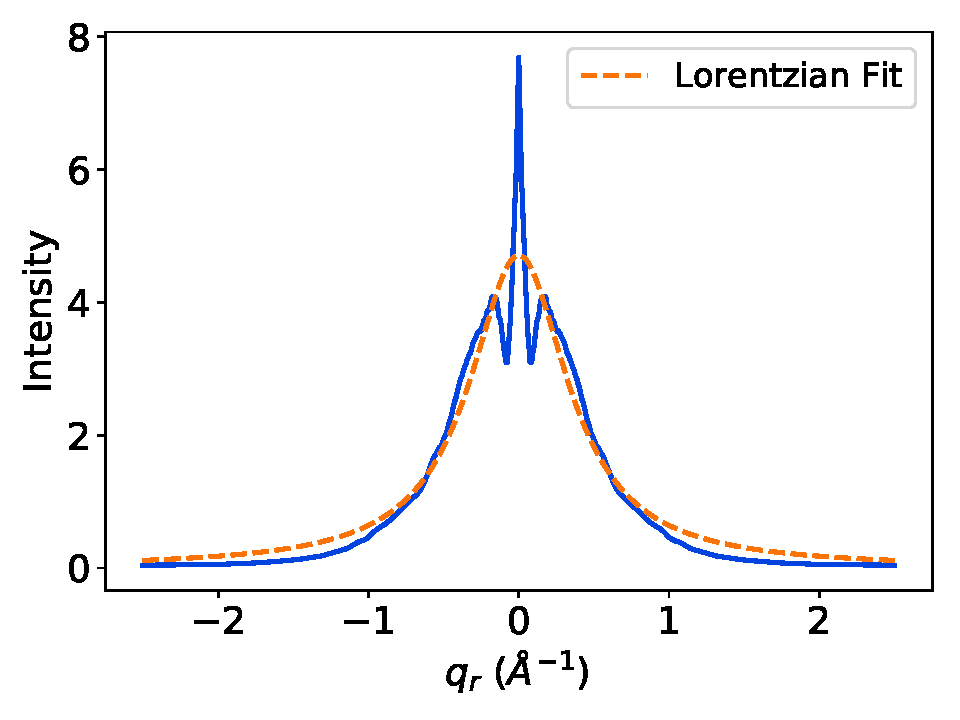
\includegraphics[width=\textwidth]{sim_rsection_fit.pdf}
  \caption{FWHM = 0.796 $\pm$ 0.011 $\AA^{-1}$}\label{fig:sim_rsection_fit}
  \end{subfigure}
  \begin{subfigure}{0.45\textwidth}
  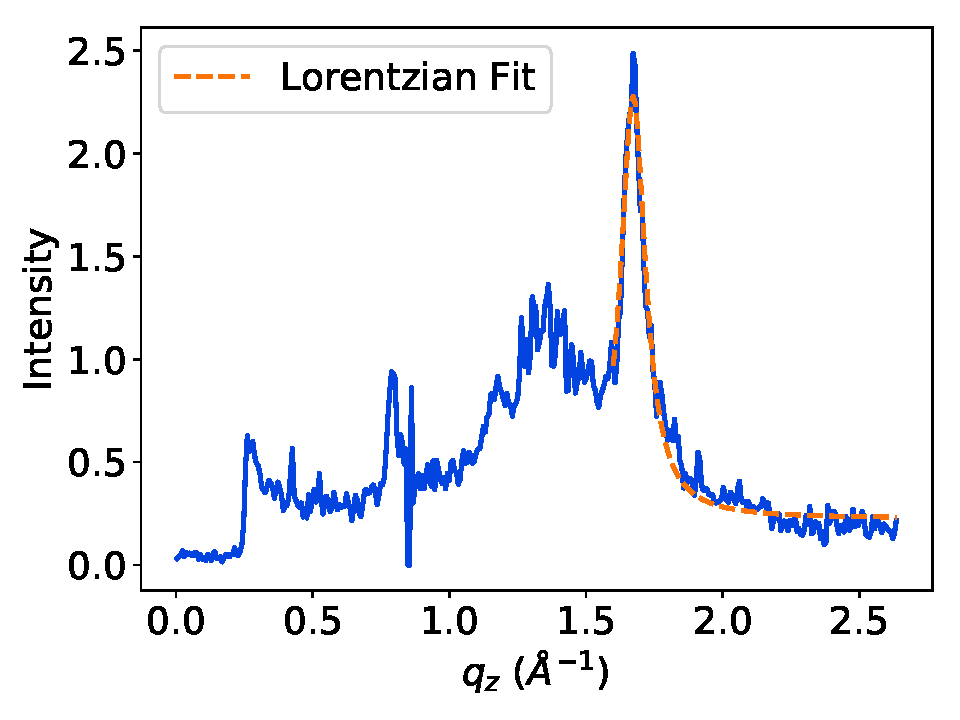
\includegraphics[width=\textwidth]{exp_zsection_fit.pdf}
  \caption{FWHM = 0.110 $\pm$ 0.003 $\AA^{-1}$}\label{fig:exp_zsection_fit}
  \end{subfigure}
  \begin{subfigure}{0.45\textwidth}
  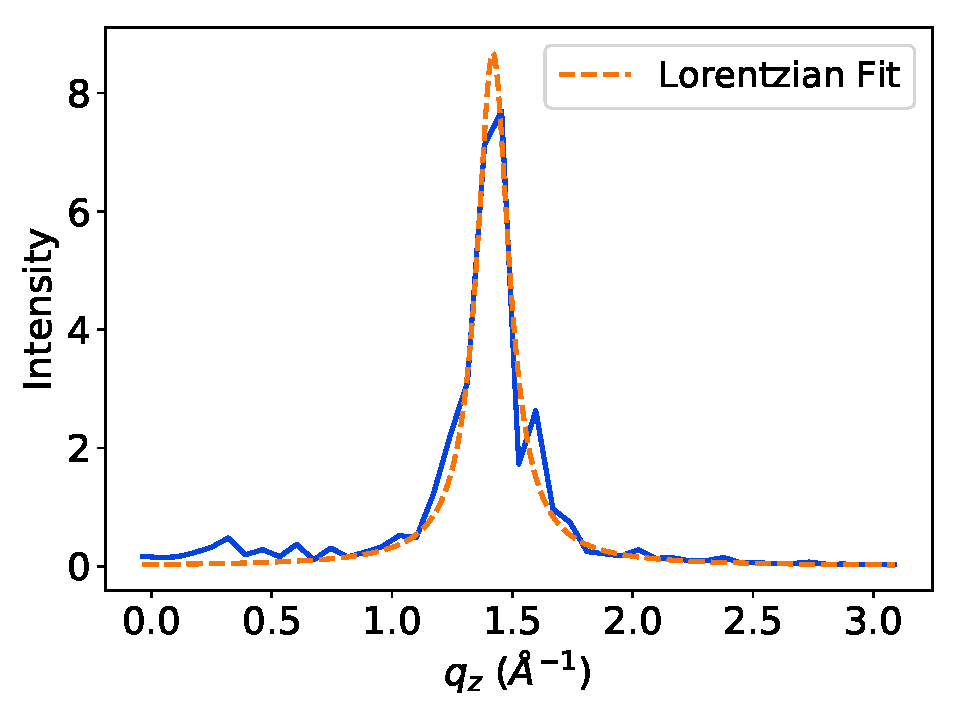
\includegraphics[width=\textwidth]{sim_zsection_fit.pdf}
  \caption{FWHM = 0.163 $\pm$ 0.011 $\AA^{-1}$}\label{fig:sim_zsection_fit}
  \end{subfigure}
  \caption{
	  The maximum intensity of R-$\pi$ generated from simulations of the ordered
	  parallel displaced configuration is 3 times larger than experiment. The $q_r$
	  cross-section of R-$\pi$ ((a) and (b)) is qualitatively different between
	  experiment (a) and simulation (b). We fit Lorentzian profiles to each peak and
	  the FWHM (full width at half maximum) of the simulated pattern agrees with
	  experiment within error. However the fit to the simulated data is affected by
	  the three sharp peaks which appear near $q_r$ = 0. The $q_z$ cross-sections of
	  R-$\pi$ ((c) and (d)) are qualitatively similar. Each fits a Lorentzian profile
	  well, however the FWHM of the simulated cross-section (d) is 48\% larger than
	  the experimental cross-section (c). Additionally, the peak of the simulated
	  $q_z$ cross-section is located at a lower $q_z$ value than
	  experiment.}\label{fig:rpi_exp_comparison}
  \end{figure}

  \subsubsection*{Distance and correlation between stacked monomer head groups}

  R-$\pi$ appears at a lower $q_z$ value in our simulations versus experiment
  because monomers in the simulated system stack further apart than those in the
  experimental system (Table~\ref{table:correlation_length}). We calculated
  $z$-direction pair distribution functions, $g(z)$, as described in
  Section~\ref{section:correlation_length}.  The resulting distributions are
  generally characterized by decaying oscillatory behavior where the average
  distance between peaks corresponds to the average distance between stacked
  monomer head groups (Figure~\ref{fig:correlation}).  We calculated this
  equilibrated vertical stacking distance, $\mathit{d}_{equil}$, between monomers
  using Equation~\ref{eqn:decaying_sinusoid}. The distance between stacked
  monomers is greater than experiment by 0.5--0.9 \AA~across all cases, with
  disordered basins at the high end of that range. This behavior is not
  surprising since GAFF models atoms as point charges and does not appropriately
  model the aromatic $\pi-\pi$ interactions, which would make it more
  energetically favorable for the monomers to stack closer together
  \cite{wang_development_2004}. It is also possible that the tails prevent
  close stacking of monomer head groups and we do not achieve the timescales
  necessary for them to rearrange into a necessarily more tightly packed
  configuration. To test this chain-packing hypotheses, we equilibrated the
  system at 500 K and then annealed it to 300 K in an attempt to coerce the tails
  into a more tightly packed configuration. Before annealing and in order to
  stabilize the hexagonal phase at 500 K, we placed harmonic restraints with
  force constants of 1000 kJ mol$^{-1}$ nm$^{-2}$ between head group COMs within
  each column as well as between head group COMs in adjacent columns. We saw no
  improvement in packing distance over our 300 K models (see further discussion
  in Section~\ref{section:slow_dynamics}). 
  
  The system size, in the $z$-direction, does not significantly alter $g(z)$.
  In Figure~\ref{fig:correlation}, oscillations do not fully decay, so a taller
  system may be necessary to fully capture the correlation function. We therefore
  equilibrated a sandwiched system with twice as many monomers per column so that
  the system size doubled in the $z$-direction. The correlation length increases
  modestly from 4.5 $\pm$ 0.4 to 7.3 $\pm$ 1.2 \AA. However, visually, the
  correlation functions are nearly identical and oscillatory behavior persists
  throughout $g(z)$ in both cases (See
  Figure \ref{S-fig:z_correlation_overlay}).

  The broadening of the $q_z$ cross-section of R-$\pi$ is related to
  $z$-directional correlation between scatters within monomer columns. The
  correlation length varies as the inverse of the full width at half maximum
  (FWHM) of the $q_z$ cross-section of R-$\pi$~\cite{young_highly_2013-1}. Using
  this technique, we calculated the correlation length of the experimental 
  system to be 9.0 \AA. As scatterers become less correlated, we expect that
  R-$\pi$ will broaden.

  The correlation lengths of vertically stacked scatterers in our atomistic
  simulations are in reasonable agreement with experiment. Since it is not
  feasible for us to simulate membranes with much taller columns in order to
  obtain increased $q_z$ resolution of our simulated XRD patterns, and because
  the simulated peak shape is convoluted by the extremely intense maximum of
  R-$\pi$, we measured correlation length by fitting
  Equation~\ref{eqn:decaying_exponential} to the peaks of $g(z)$. The correlation
  length of the parallel displaced, ordered basin system shows the closest
  agreement with experiment (Table~\ref{table:correlation_length}). 
  We could not extract a reliable correlation length from the disordered
  parallel displaced configuration since the peaks do not show clear patterns
  that can easily be fit to an exponential decay. The correlation length of both
  sandwiched systems are relatively low because the height of the first peak of
  $g(z)$ is so high. 
  
  Overall, we believe our simulations exhibit a realistic amount of distance
  correlation in the direction parallel to the pore axis between head groups
  within each column. The difference in the FWHM of the $q_z$ cross-section of
  R-$\pi$ between experiment and simulation is less than one bin size
  (Figures~\ref{fig:exp_zsection_fit} and~\ref{fig:sim_zsection_fit}). The more
  significant difference between the two cross-sections is their maximum intensity
  which we study in more detail below.
  
  \begin{figure}[!htb]
  \centering
  \begin{subfigure}{0.45\textwidth}
  \centering
  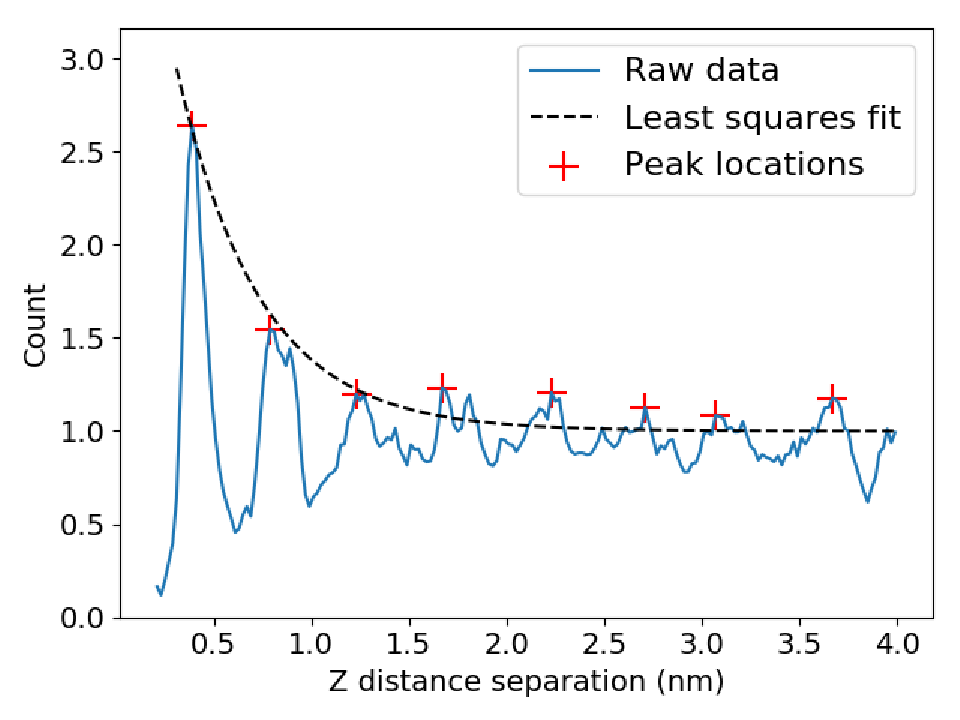
\includegraphics[width=\textwidth]{z_correlation_sandwich.pdf}
  \caption{Sandwiched, Ordered Basin}\label{fig:z_correlation_sandwich}
  \end{subfigure}  
  \begin{subfigure}{0.45\textwidth}
  \centering
  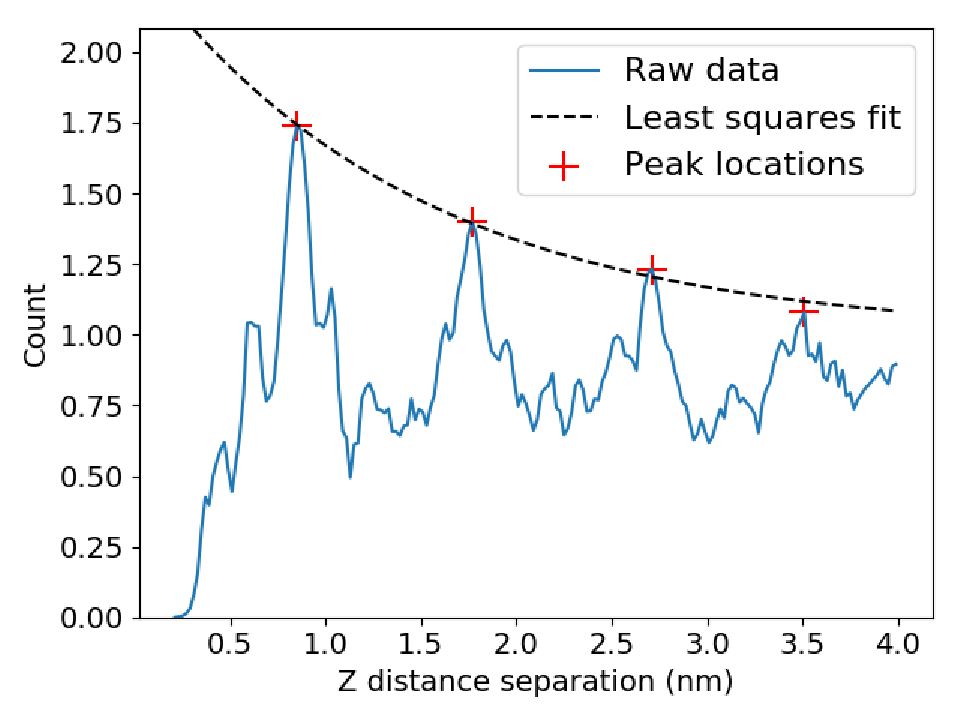
\includegraphics[width=\textwidth]{z_correlation_offset.pdf}
  \caption{Parallel Displaced, Ordered Basin}\label{fig:z_correlation_offset}
  \end{subfigure}  
  \begin{subfigure}{0.45\textwidth}
  \centering
  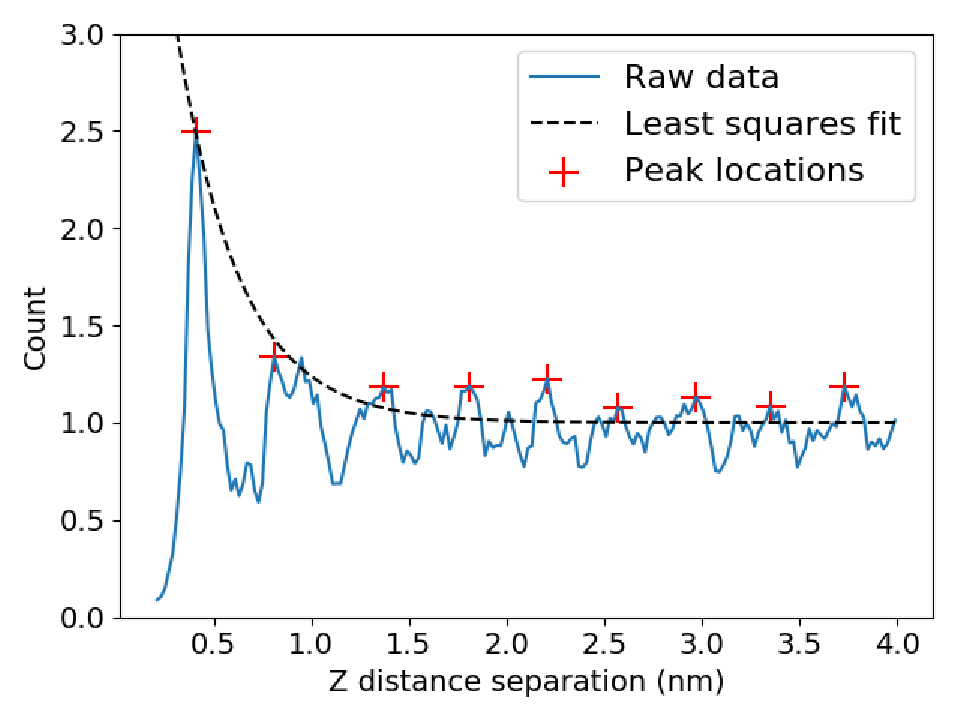
\includegraphics[width=\textwidth]{z_correlation_sandwich_disordered.pdf}
  \caption{Sandwiched, Disordered Basin}\label{fig:z_correlation_sandwich_disordered}
  \end{subfigure}  
  \begin{subfigure}{0.45\textwidth}
  \centering
  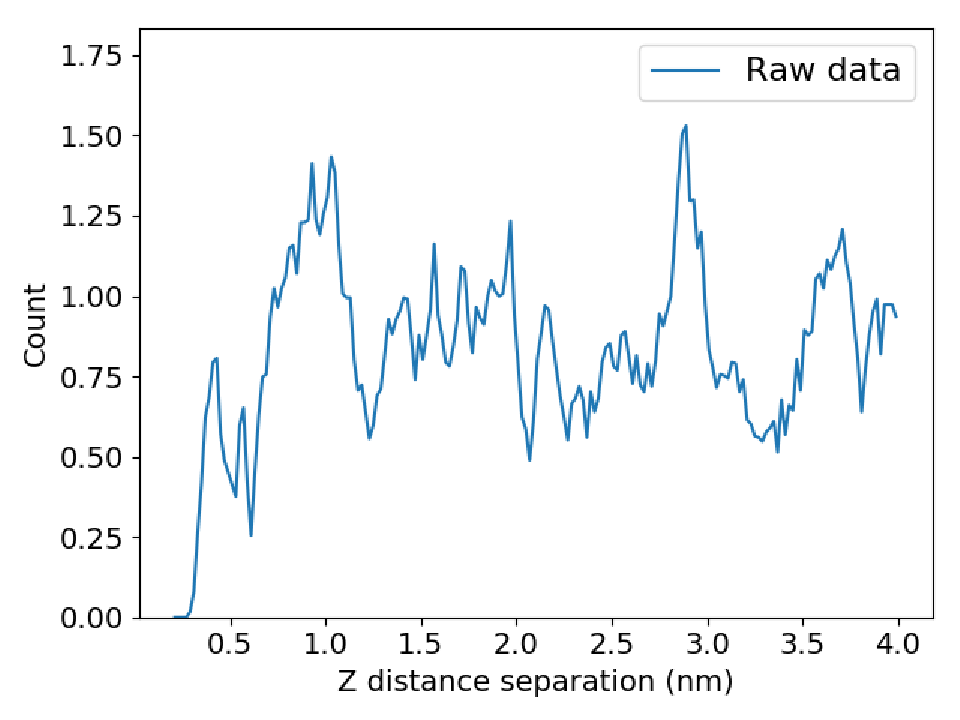
\includegraphics[width=\textwidth]{z_correlation_offset_disordered.pdf}
  \caption{Parallel Displaced, Disordered Basin}\label{fig:z_correlation_offset_disordered}
  \end{subfigure}  
  \caption{1D correlation functions of the center of masses of aromatic head
	  groups, $g(z)$, show decaying oscillatory behavior and have consistent
	  correlation lengths with experiment. We calculated the correlation length by
	  fitting a decaying exponential function
	  (Equation~\ref{eqn:decaying_exponential}) to the peaks of $g(z)$. The
	  correlation length is longer for ordered basin systems
	  (Table~\ref{table:correlation_length}). We did not attempt to calculate the
	  correlation length for (d) because there are no clear peaks. We assume that
	  this correlation length is less than the vertical distance between
	  monomers.}\label{fig:correlation}
  \end{figure}  
  
  \begin{table}[h]
  \centering
  \begin{tabular}{cccc}
  \toprule
  System             & $\mathit{d}$ (\AA) & $\mathit{d}_{equil}$ (\AA) & Correlation Length (\AA) \\
  \midrule
  Sandwiched         & 3.7                &    4.27 $\pm$ 0.03         & 4.2 $\pm$ 0.8            \\
  Parallel Displaced & 3.7                &    4.33 $\pm$ 0.04         & 14.5 $\pm$ 1.3           \\ 
  Sandwiched         & 5.0                &    4.48 $\pm$ 0.07         & 3.2 $\pm$ 0.9            \\
  Parallel Displaced & 5.0                &    4.60 $\pm$ 0.08         & $<$ $d_{equil}$ \\ 
  Experiment         & --                 &    3.70                    & 9 $\pm$ 1               \\
  \bottomrule
  \end{tabular}
  \caption{The correlation length is larger for systems in the ordered basin.
	  The equilibrated vertical stacking distance, $\mathit{d}_{equil}$, is also
	  smaller.}
  \label{table:correlation_length}
  \end{table}

  \subsubsection*{Shape and Intensity of the $q_r$ cross-section of R-$\pi$}

  In addition to the maximum intensity of R-$\pi$ being too high, the shape
  of its $q_r$ cross-section in the simulated XRD is qualitatively different
  from experiment (Figures~\ref{fig:exp_rsection_fit}
  and~\ref{fig:sim_rsection_fit}). We attempted to fit a Lorentzian profile to 
  the $q_r$ cross-section and although the FWHM agrees with experiment within
  error, the fit is not optimal due to the three sharp peaks that appear near
  $q_r$ = 0. 
  
  An exact quantitative comparison between the intensity and FWHM of the
  experimental and simulated cross-sections of R-$\pi$ is not feasible for
  several reasons. Experimental peaks broaden due to effects that we can not
  easily simulate such as finite size crystalline domains and instrumental % reference needed
  resolution~\cite{girolami_x-ray_2016}. In our simulated XRD patterns, 
  the system size imposes limitations
  on the resolution, which makes it difficult to reliably fit peaks. This is
  especially problematic when comparing the FWHM of the $q_z$ cross-section of
  R-$\pi$, where the experimental FWHM (0.11 $\AA^{-1}$) is similar to the bin
  size in the $q_z$ direction (ca. 0.07 $\AA^{-1}$).  Additionally, we model each
  atom with a Gaussian sphere of electron density, which is a simplification.
  However, we can explore reasons for which differences in the simulation
  structure could change the peak shapes and intensities to be in better
  agreement with experiment.
   
  We studied the shape and intensity of R-$\pi$ by setting up simplified
  systems where we represent monomer head groups as point scatterers, as
  described in Section~\ref{method:simple_systems}. The amount of quenched and
  thermal disorder present in the atomistic system, which we applied to the
  simplified systems, are given in Table~\ref{table:quenched_disorder}. The
  quenched disorder, the deviation of monomers from idealized symmetric
  configurations, is several times greater than thermal disorder, the 
  deviations of the monomers from their average positions during the 
  production simulations.
  
  \begin{table}[h]
  \centering
  \begin{tabular}{c|ccc|ccc}
  \toprule
   		                        &           \multicolumn{3}{c}{Thermal Disorder}             &             \multicolumn{3}{c}{Quenched Disorder}               \\
  \midrule
  System                        & $\sigma_x$ ($\AA$) & $\sigma_y$ (rad) & $\sigma_z$ ($\AA$) & $\sigma_z$ ($\AA$) & $\sigma_\theta$ (rad) & $\sigma_r$ ($\AA$) \\
  \midrule
  Ordered Sandwiched            &         0.31       &       0.33       &        0.34        &        1.48        &     0.43              &     2.30           \\
  Ordered Parallel Displaced    &         0.51       &       0.52       &        0.30        &        1.45        &     0.43              &     2.28           \\ 
  Disordered Sandwiched         &         0.41       &       0.57       &        0.32        &        1.58        &     0.43              &     2.93           \\
  Disordered Parallel Displaced &         0.39       &       0.31       &        0.33        &        1.65        &     0.43              &     2.63           \\
  \bottomrule
  \end{tabular}
  \caption{Deviation of the positions of the center of mass of head groups from their average
  positions (thermal disorder) as well as their idealized positions (quenched disorder) to use 
  as simulated disorder in our model system.}
  \label{table:quenched_disorder} 
  \end{table}
  
  Increasing thermal noise in the $z$-direction will reduce the intensity
  of R-$\pi$, however the $q_r$ profile remains unchanged. When we increased the
  thermal noise of the simplified parallel displaced system in the $z$-direction by
  12\% and 27\%, we saw a 3 and 15-fold decrease in the maximum intensity of 
  R-$\pi$ respectively (Figure~\ref{fig:znoise}). Despite the decrease in 
  intensity, the 3 cross-sections have the same shape 
  (Figure~\ref{fig:rpi_xsection_vs_zsigma}), whose sharp Bragg-like peaks are
  not consistent with experiment. 
  
  \begin{figure}[!htb]
  \centering
  \begin{subfigure}{0.49\textwidth}
  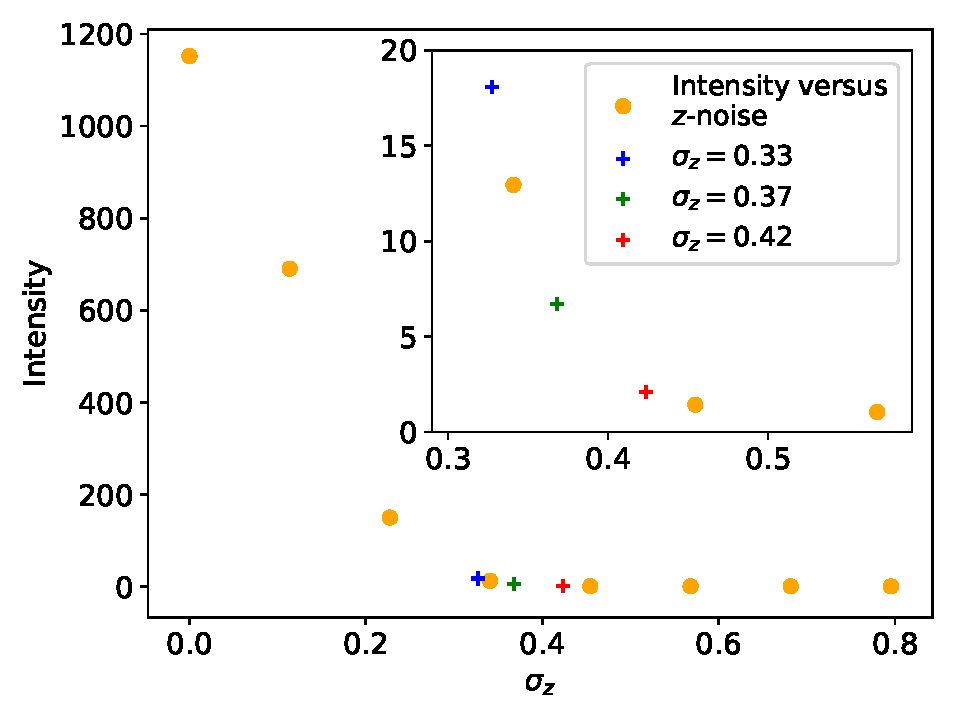
\includegraphics[width=\textwidth]{intensity_vs_zsigma.pdf}
  \caption{}\label{fig:intensity_vs_zsigma}
  \end{subfigure}
  \begin{subfigure}{0.49\textwidth}
  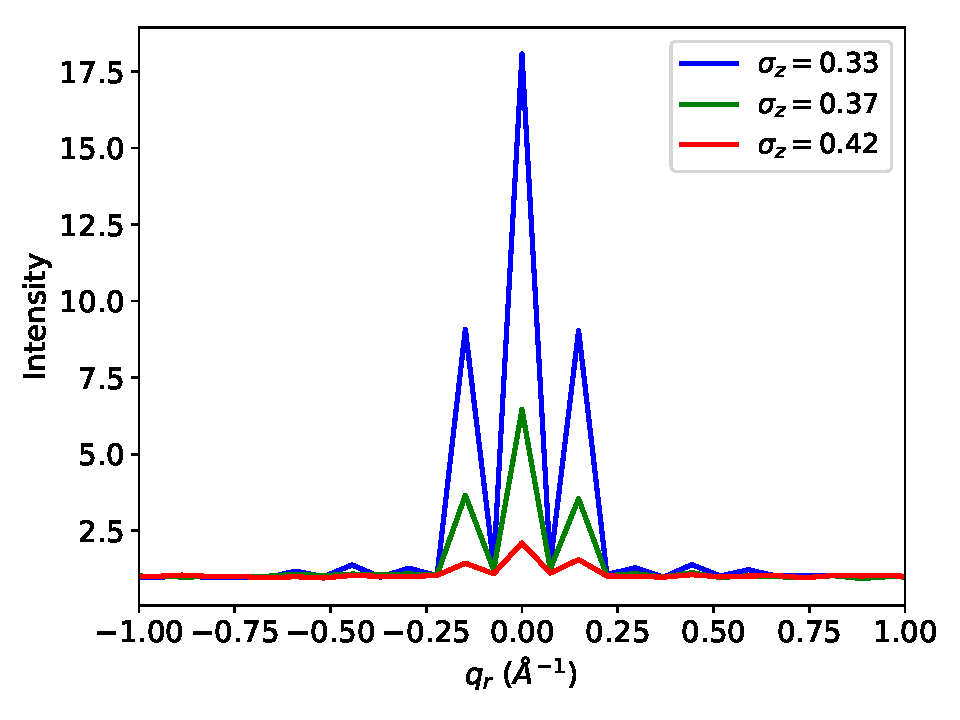
\includegraphics[width=\textwidth]{rpi_xsection_vs_zsigma.pdf}
  \caption{}\label{fig:rpi_xsection_vs_zsigma}
  \end{subfigure}
  \caption{We can decrease the maximum intensity of R-$\pi$ by increasing
  thermal noise in the $z$-direction; however, the $q_r$ cross-section profile does
  not change. (a) The intensity of R-$\pi$ drops precipitously as we increase
  $\sigma_z$. We can decrease the intensity of R-$\pi$, relative to the
  background intensity, relative to systems with simulation levels of disorder (blue)
  by a factor of 3 when we increase $\sigma_z$ by 12\% (green) and by a factor 
  of 15 when we increase $\sigma_z$ by 27\% (red). (b) Although the maximum intensity of R-$\pi$
  decreases with increasing $\sigma_z$, the peak shape remains the same.}\label{fig:znoise}
  \end{figure}
  
  However, when we allowed monomer columns to move independently in the
  $z$-direction, the intensity of R-$\pi$ drops and the $q_r$ cross-section of
  the simulated diffraction patterns smooths out. We can demostrate this by
  creating a simplified sandwiched configuration (as described above), with
  varying amounts of statistical correlation between columns (see
  Figure~\ref{fig:column_displacement}). In the low independent motion limit, the
  COM of columns are situated at the same $z$-coordinate.  We allow increasing
  independence of columns by randomly shifting each column in the $z$-direction
  according to a uniform distribution bounded by (0, $f \times \mathit{d}$) where
  $f$ ranges between 0 and 1 and $d$ is the vertical distance between scatterers.
  When $f = 1$, the columns move independently and the $q_r$ cross-section
  smooths out completely (Figure~\ref{fig:sf_qy_sr100}). Any amount of dependence
  results in some presence of sharp peaks, though significantly attenuated at $f$
  nearer 1. The intensity of R-$\pi$ also decreases with increasing column
  independence. We see an 9-fold decrease in the intensity of R-$\pi$ when $f=1$
  versus when $f=0$ for our simplified model systems.

  % produce figures with: structure_factor.py --random_columns -nframes 1000 --hexagonal -g 86 86 256 -thermal_disorder 2.30 0.43 1.48 -dbwl 4.4 --pore_radius 6.6 -box 85 85 352 -sr 0
  % Adjust sr from 0 to .75 to 1
  \begin{figure}
  \centering
  \begin{subfigure}{0.325\textwidth}
  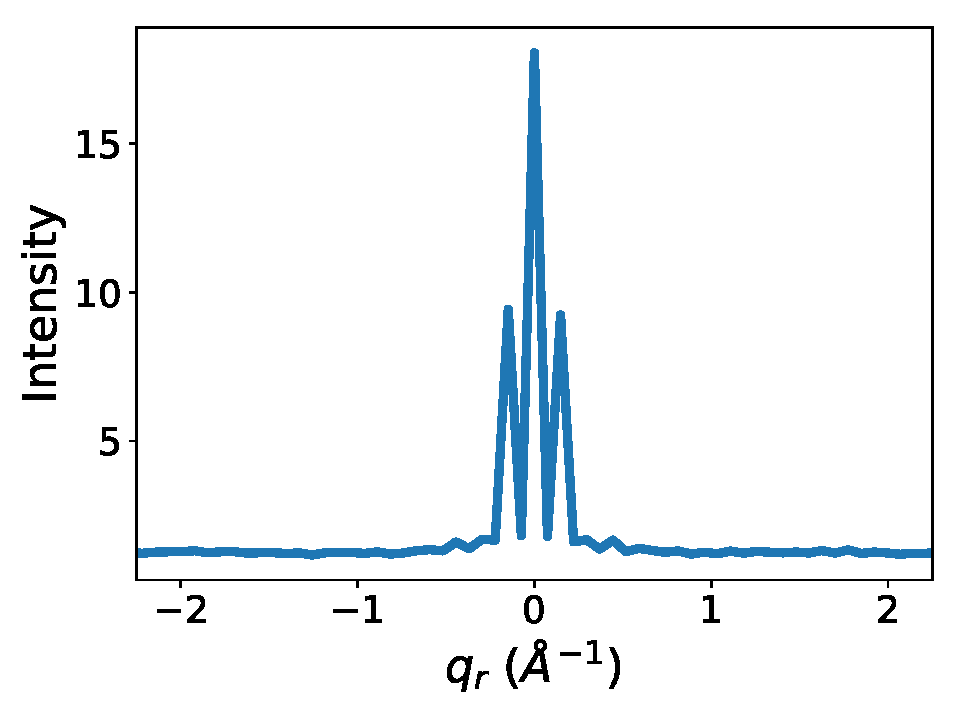
\includegraphics[width=\textwidth]{sf_qy_sr0.pdf}
  \caption{$f$ = 0}\label{fig:sf_qy_sr0}
  \end{subfigure}
  \begin{subfigure}{0.325\textwidth}
  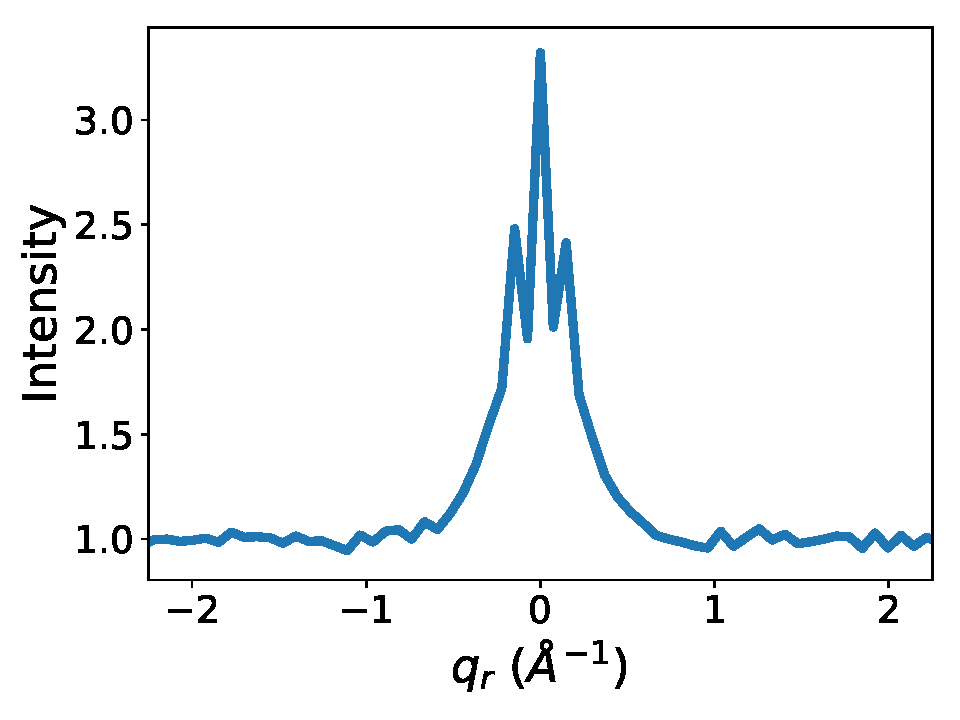
\includegraphics[width=\textwidth]{sf_qy_sr75.pdf}
  \caption{$f$ = 0.75}\label{fig:sf_qy_sr75}
  \end{subfigure}
  \begin{subfigure}{0.325\textwidth}
  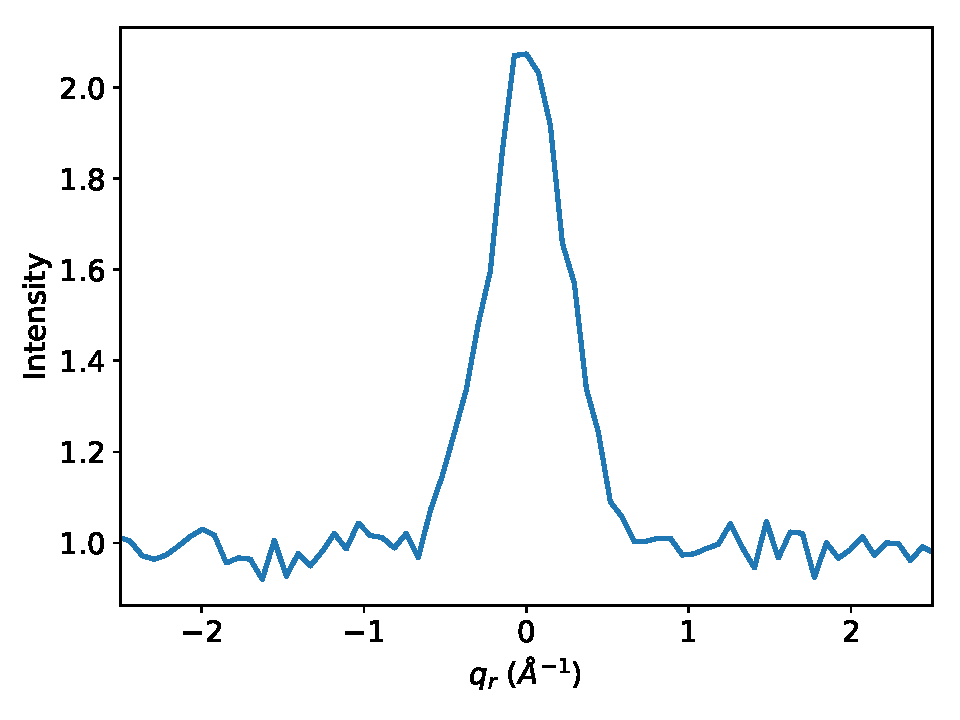
\includegraphics[width=\textwidth]{sf_qy_sr100.pdf}
  \caption{$f$ = 1}\label{fig:sf_qy_sr100}
  \end{subfigure}
  \caption{As we increase column independence using the $f$ parameter, the
	  intensity of R-$\pi$ decreases and the $q_r$ cross-section of the simulated
	  diffraction pattern becomes more smooth.  (a) When we place all columns at the
	  same reference $z$ coordinate, $f$ = 0, the intensity of R-$\pi$ is 18.3 and is
	  characterized by sharp Bragg-like peaks. (b) When columns have a moderate
	  amount of independence, $f$ = 0.75, the intensity of R-$\pi$ decreases 5-fold
	  to 3.4. The edges of the peak are beginning to smooth out, but sharp peaks
	  still exist. (c) When columns are completely independent, $f$ = 1, the
	  intensity of R-$\pi$ decreases 9-fold to 2.1 and the cross-section is
          relatively smooth.}\label{fig:column_displacement}
  \end{figure}

  It therefore seems likely that the discrepancy between the shape and intensity of
  R-$\pi$ generated from our simulations versus experiment is primarily due to
  highly correlated columns in our highly symmetric initial configurations.
  If the columns were uncorrelated, $g(z)$ of the ordered sandwiched system 
  would very closely resemble Figure~\ref{fig:z_correlation_sandwich} when we 
  average all $z$-slices of the 3D correlation function. Contributions to
  $g(z)$ from head groups in other columns within the same pore, and with head
  groups in different pores would cancel out. However, when we include all 
  $z$-slices in $g(z)$ for our system, rather than restricting it to those 
  $z$-slices within 2.1~\AA~of the center of the correlation function 
  (Section~\ref{section:correlation_length}), $g(z)$ shows oscillatory 
  behavior and its correlation length nearly triples to 12.4 $\pm$ 0.7 \AA.
  (Figure~\ref{fig:z_correlation_fullbox}). The peaks of $g(z)$ are actually 
  reinforced by head groups in neighboring columns which is not expected
  in a system where columns act independently.

  \begin{figure}
  \centering
  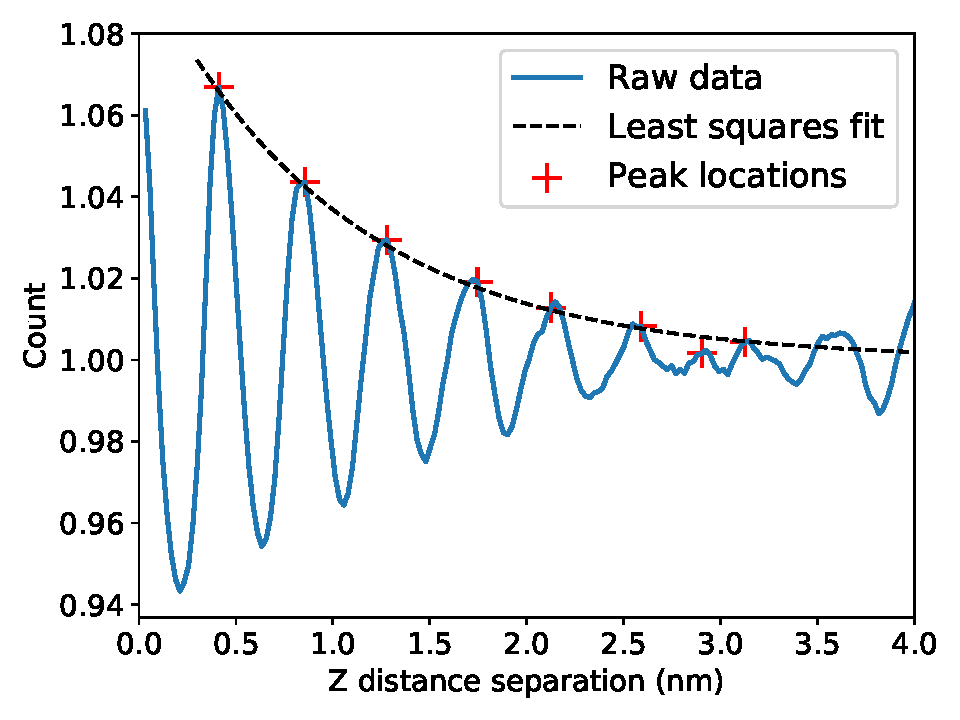
\includegraphics[width=0.5\textwidth]{z_correlation_fullbox.pdf}
  \caption{When we average all $z$-slices of the 3D correlation function, the 
  correlation length of the ordered sandwich configuration nearly triples compared 
  to that shown in Figure~\ref{fig:z_correlation_sandwich}.}\label{fig:z_correlation_fullbox}
  \end{figure}
 
  Increasing thermal noise in the $xy$ plane causes the FWHM of the $q_r$
  cross-section of R-$\pi$ to, somewhat counterintuitively, decrease. Using a
  system with uncorrelated columns, we modified the disorder in both the $r$ and
  $\theta$ directions by multiplying their values by a factor of 0.5 and 2
  (Figure~\ref{fig:qy_fwhm}). When we cut the noise in half, the FWHM increases
  by 88\%. When we double the noise, the FWHM decreases by 51\%. As we have fit
  the data in Figure~\ref{fig:sim_rsection_fit}, the FWHM of R-$\pi$ agrees well
  with experiment, meaning the quenched configuration contains about the right
  amount of disorder on the $xy$ plane. However, the relatively low quality of
  the fit implies that the FWHM of a fixed Lorentzian fit to data from a single
  simulation might not be the best comparison to experiment and that some form of
  initial configuration dependence causes extra structure.

  \begin{figure}
  \centering
  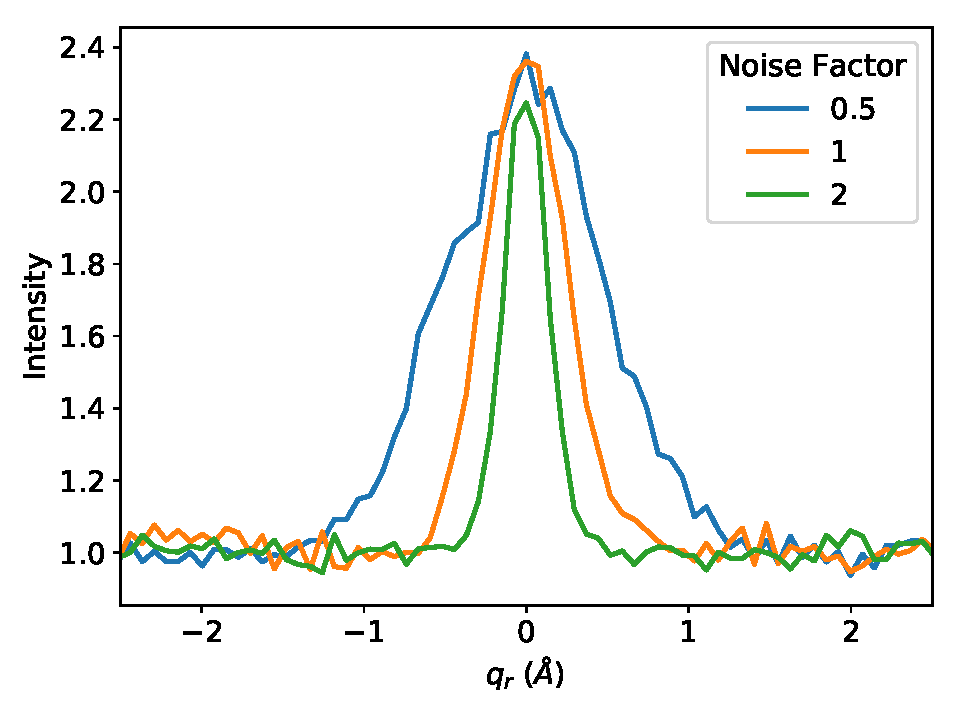
\includegraphics[width=0.5\textwidth]{qy_fwhm.pdf}
  \caption{Increasing the amount of disorder in the $xy$ plane decreases the
	  FWHM of the $q_r$ cross-section of R-$\pi$. When we cut the amount of $r$ and
	  $\theta$ disorder in half (Noise factor = 0.5), the FWHM increases by 88\%. When
	  we double the disorder (Noise factor = 2), the FWHM decreases by
	  51\%.}\label{fig:qy_fwhm}
  \end{figure}
  
  \subsubsection*{Quenched disorder in ensembles of configurations}  

  Since the dynamics of this system are slow, consequently most of our analysis
  has been focused on a set of quenched configurations with some structural
  characteristics that do not vary significantly with time. We therefore
  attempted to learn more about their time-averaged structures by studying
  ensembles of shorter simulations started from more independent initial
  configurations. To do this, we created ensembles of 40 simulations in both the
  parallel displaced and sandwiched configurations. We used the same
  equilibration scheme described in Section~\ref{section:equilibration}.
  However, we built the initial configurations with columns randomly displaced in
  the $z$-direction and looked at the results after 5 ns of unrestrained
  simulation, which should capture any quenched disorder built in from the
  initial configurations. We then simulated XRD patterns from the 40
  trajectories, concatenated together. The $q_r$ cross-sections of R-$\pi$
  generated from the two concatenated trajectories are shown in
  Figure~\ref{fig:ensemble_XRD}. 
  
  Qualitatively, the $q_r$ cross-sections of R-$\pi$ generated from ensembles of
  simulations are nearly smooth, with only small spikes near $q_r$=0. These data
  suggest that the average intensity of R-$\pi$ in the ensemble of sandwiched 
  systems is about 3$\times$ higher than that in the ensemble of parallel displaced
  configurations. Compared to our long simulations, the intensity of R-$\pi$
  generated from ensembles of short simulations decreases by a factor of 3
  and by a factor of 2 for the sandwiched and parallel displaced configurations respectively. 

  Overall, the intensity of R-$\pi$ generated from the parallel displaced 
  ensemble of short simulations shows the best agreement with experiment so far. For simplicity, 
  we will limit the following discussion to the parallel displaced configuration.
  Data for the sandwiched configuration is presented in Section 
  \ref{S-section:sandwiched_ensemble}.

  \begin{figure}[!htb]
  \centering
  \begin{subfigure}{0.45\textwidth}
  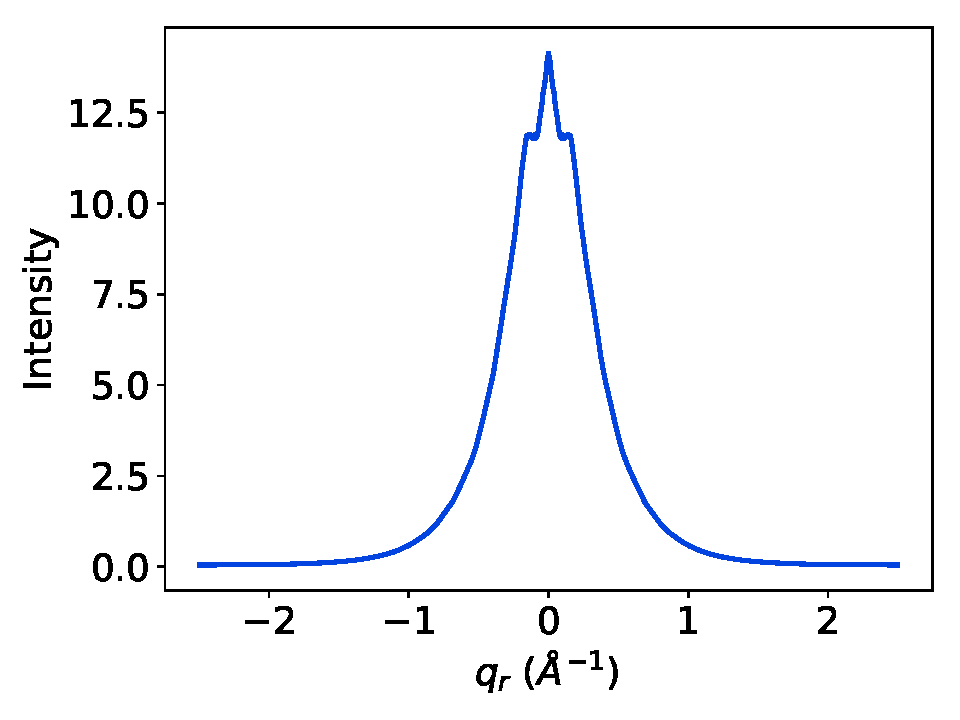
\includegraphics[width=\textwidth]{sandwiched_ensemble_rsection.pdf}
  \caption{Sandwiched}\label{fig:sandwiched_ensemble_rsection}
  \end{subfigure}
  \begin{subfigure}{0.45\textwidth}
  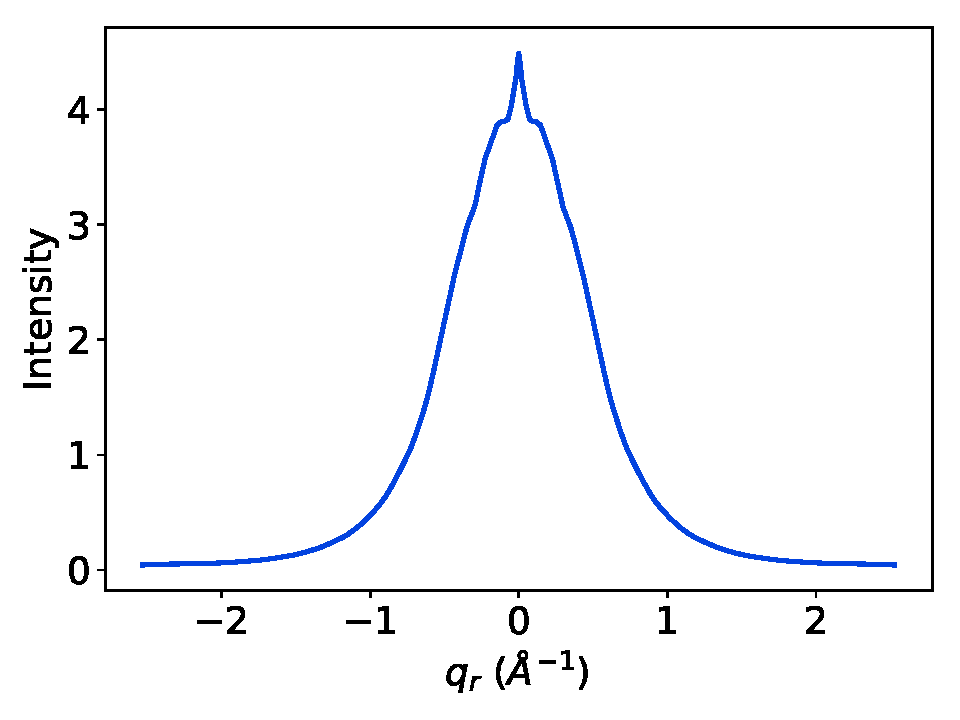
\includegraphics[width=\textwidth]{offset_ensemble_rsection.pdf}
  \caption{Parallel Displaced}\label{fig:offset_ensemble_rsection}
  \end{subfigure}
  \caption{The $q_r$ section of R-$\pi$ is much smoother than Figure~\ref{fig:sim_rsection_fit} when
  		   we generate simulated XRD patterns from an ensemble of 40 independent simulations,
  		   suggesting that much of the extra initial intensity may be due to the starting 
  		   conditions. The maximum intensity of R-$\pi$ is 3$\times$ higher in the sandwiched
  		   configuration (a) than in the parallel displaced configuration (b).}\label{fig:ensemble_XRD}
  \end{figure}
 
  These short independent simulations exhibit a symmetric distribution of
  quenched disorder providing evidence that the quenched disorder is randomized
  in each system.  The only difference between each independent initial
  configuration is the random $z$-direction displacement that we apply to each
  column. The quenched disorder is then a result of the initial structural
  collapse that is directed by the randomized velocity vectors of the system's
  atoms drawn from a Maxwell-Boltzmann distribution. We pooled the deviations of
  each head group COM from idealized positions from all independent simulations
  in order to create the distributions shown in
  Figure~\ref{fig:offset_ensemble_pooled} (see
  Section~\ref{method:simple_systems}). The distributions appear symmetric
  meaning that there is an equal chance for a head group to displace in the
  positive or negative $z$, $r$, or $\theta$-direction.

  We verified that this same symmetry exists for individual COMs.  If we
  consider the COM of a given head group, we expect that the distribution of its
  deviations from its idealized position among all the independent simulations
  should be symmetric about its idealized position. We can calculate the
  empirical cumulative distribution function (ECDF) of these distributions of
  deviations. The ECDFs of 3 randomly selected COMs are shown in
  Figure~\ref{fig:offset_ecdfs} to guide the eye (colored lines). The average of
  all COM ECDFs is represented by the red line with the 95\% confidence interval
  represented by the red error bars. We also calculated the ECDF from the full
  distributions in Figure~\ref{fig:offset_ensemble_pooled} (black line with error
  bars). We generated error bars that represent the 95\% confidence intervals by
  performing 1000 trials where we randomly sampled 40 values (the same as the
  number of independent simulations) from the distributions in
  Figure~\ref{fig:offset_ensemble_pooled}, then measured the deviation between
  the sampled ECDF and the full ECDF. These error bars are generally smaller than
  those generated from the 400 COM ECDFs, as there is a wider distribution of
  mean COM deviations than the mean deviations from distributions sampled from
  the full distribution. The similarity between entirely independently sampled
  ECDFs and the ECDFs from individual independent simulations supports the
  hypothesis that each quenched configuration is random and mostly independent.
  
  \begin{figure}[!htb]
  \centering
  \begin{subfigure}{\textwidth}
  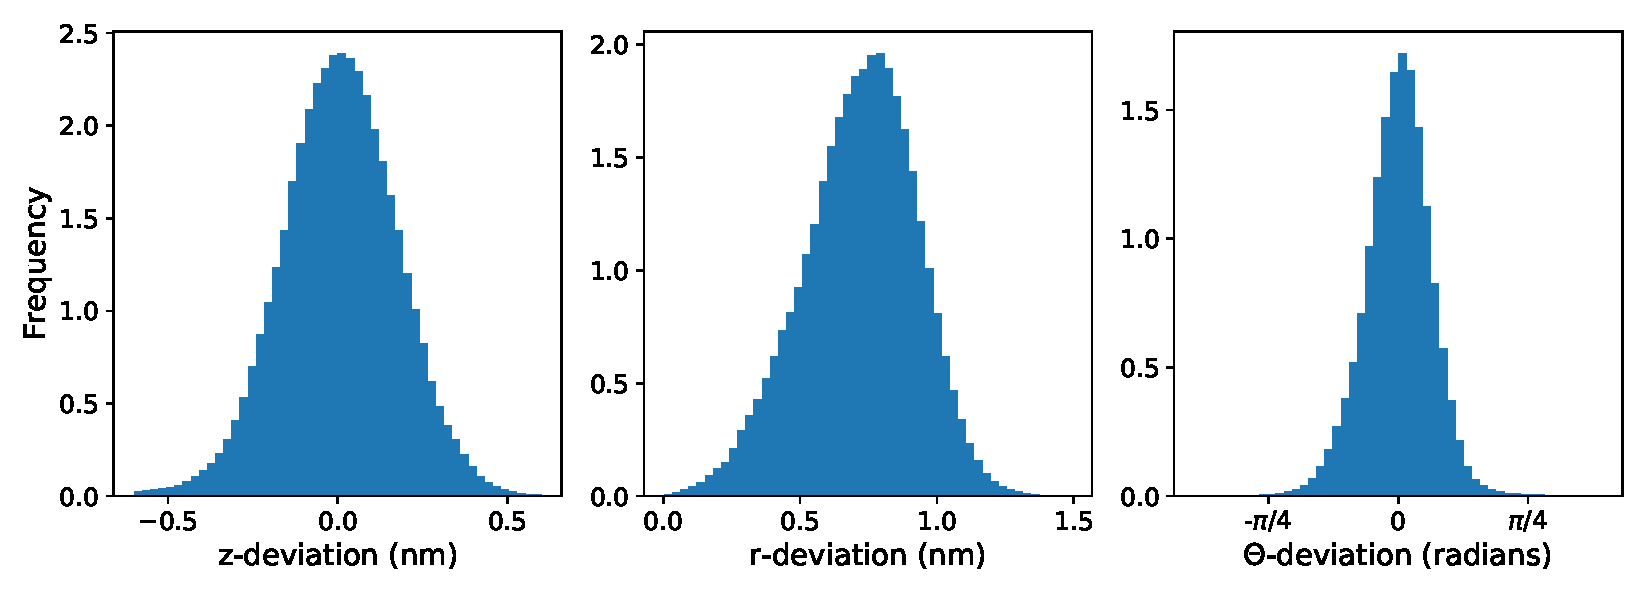
\includegraphics[width=\textwidth]{offset_ensemble_pooled.pdf}
  \caption{Distributions of deviations from ideal positions generated with data
  from all independent simulations}\label{fig:offset_ensemble_pooled}
  \end{subfigure}
  \begin{subfigure}{\textwidth}
  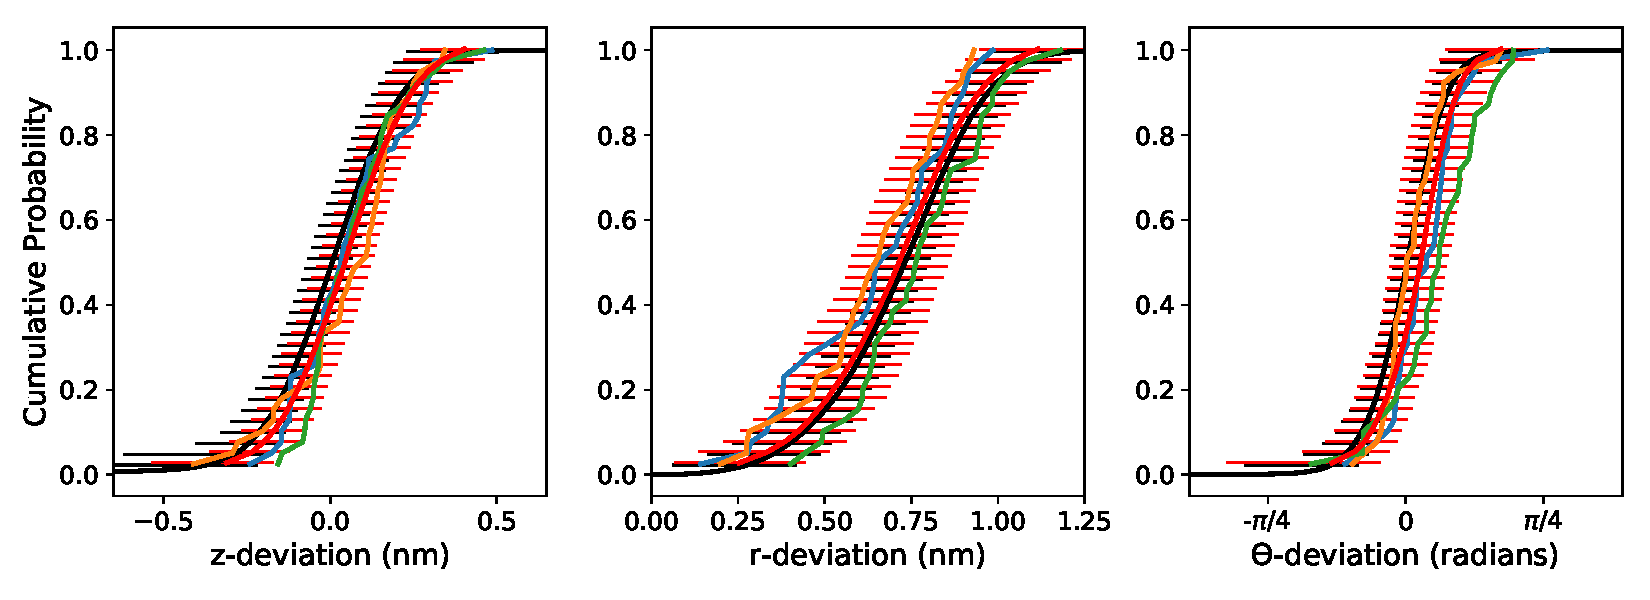
\includegraphics[width=\textwidth]{offset_ecdfs.pdf}
  \caption{Empirical cumulative distribution functions generated from (a) and
  from simulation ensembles.}\label{fig:offset_ecdfs}
  \end{subfigure}
  \caption{(a) The distributions of the head group COM deviations
  from their idealized positions generated using pooled data from all
  frames of each independent configuration are symmetric, implying that 
  there is equal probability for a head group to displace in the positive
  or negative $z$, $r$ or $\theta$-direction. (b) The COM position of a 
  given head group is displaced randomly upon quenching. The ECDF generated from
  the pooled distributions (black) in (a) agree with the means of the 
  ECDFs generated from each COM (red). The red error bars are larger than
  the black error bars since there is a wider distribution of mean COM
  deviations than the mean deviations of distributions sampled from the full
  distribution.}\label{fig:full_ensemble_distributions}
  \end{figure}
  
  The systems that we simulated for 400 ns and then used for most of our
  analysis are representative of the long term simulation behavior of any
  system chosen from the ensemble. The distributions of standard deviations 
  generated from each of the ensemble trajectories 
  (Figures~\ref{fig:offset_ensemble_stds} and~\ref{fig:offset_ensemble_means}) 
  are fairly tight with ($\sigma_{\sigma_z}$, $\sigma_{\sigma_r}$, $
  \sigma_{\sigma_\theta}$) = (0.011 nm, 0.007 nm , 0.022 radians).
  We analyzed the first 5 ns of the 400 ns ordered parallel displaced
  configuration and observed the same amount of disorder (based on the $\sigma$
  values in Figure~\ref{fig:offset_ensemble_stds}) with indistinguishable 
  mean values. Additionally, we calculated the radial density of monomer
  components as a function of their distance from the pore centers 
  (Figure~\ref{fig:offset_ensemble_regional_density}).
  All simulations have similar profiles. The distribution of sodium ions near the
  pore center is relatively noisy since the sodium ions have much more 
  translational freedom than the head groups. 
  
  \begin{figure}[!htb]
  \centering
  \begin{subfigure}{0.49\textwidth}
  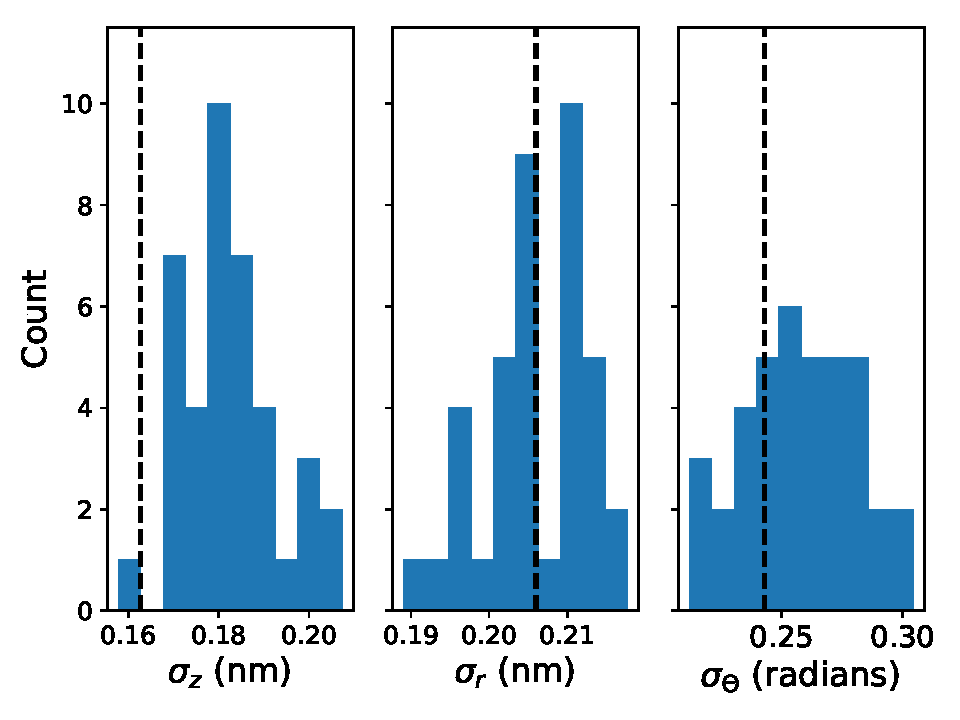
\includegraphics[width=\textwidth]{offset_ensemble_stds.pdf}
  \caption{}\label{fig:offset_ensemble_stds}
  \end{subfigure}
  \begin{subfigure}{0.49\textwidth}
  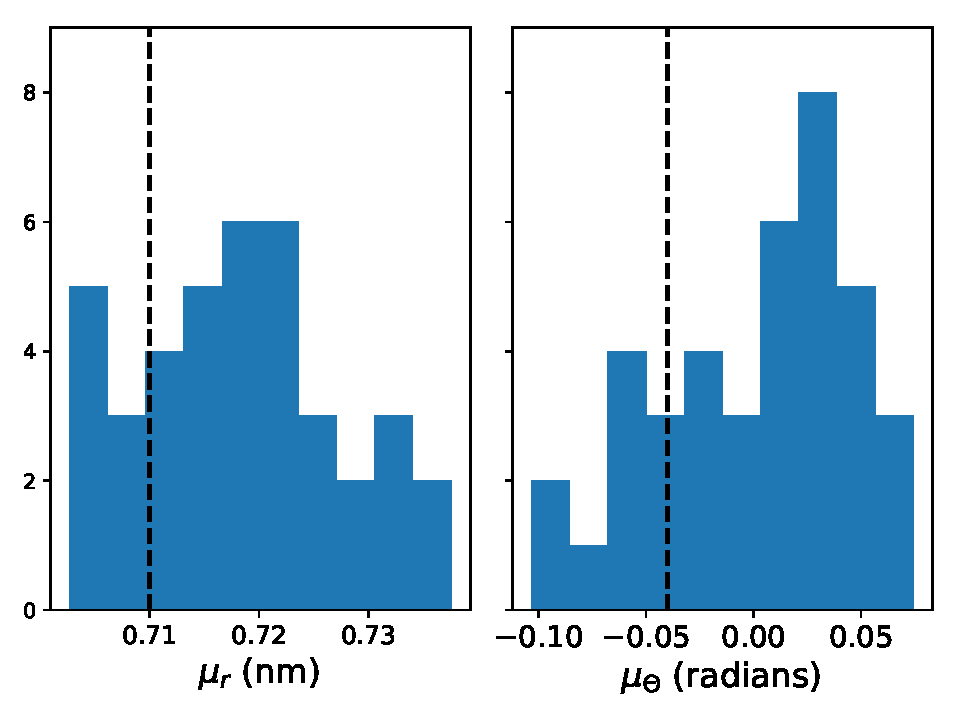
\includegraphics[width=\textwidth]{offset_ensemble_means.pdf}
  \caption{}\label{fig:offset_ensemble_means}
  \end{subfigure}
  \begin{subfigure}{\textwidth}
  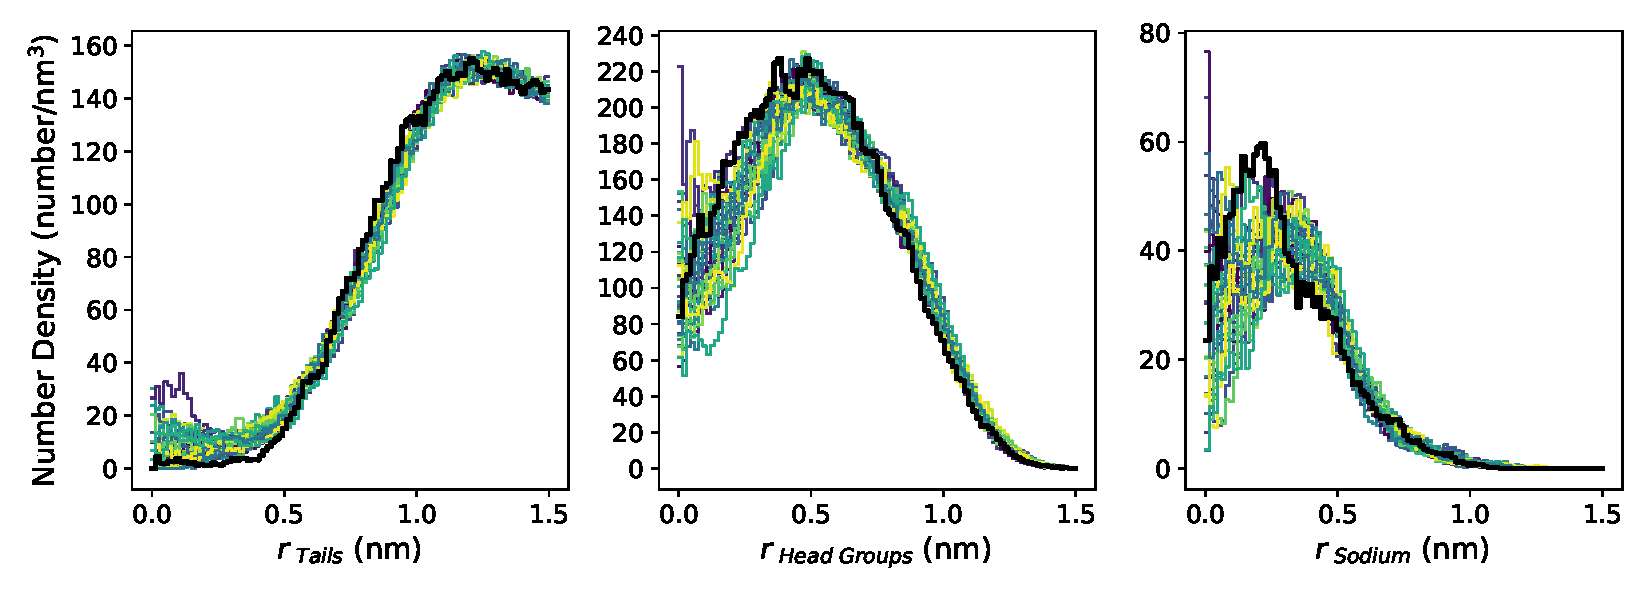
\includegraphics[width=\textwidth]{offset_ensemble_regional_density.pdf}
  \caption{}\label{fig:offset_ensemble_regional_density}
  \end{subfigure}
  \caption{(a) The standard deviation of the distribution of quenched disorder
  from the first 5 ns of the main ordered parallel displaced system studied in
  this paper (black dashed line) is in agreement with the distribution of quenched disorder 
  standard deviations calculated from the ensemble of simulations (histogram). 
  (b) The mean values of $r$ and $\theta$ from the first 5 ns of the main
  system trajectory (black dashed line) is in agreement with the distribution of mean values
  calculated from each simulation in the ensemble (histogram). The mean values of $z$
  are necessarily 0 so they are not plotted. (c) The radial densities of tail
  atoms, head group atoms and sodium atoms calculated from the first 5 ns of the
  main system simulation trajectory (black lines) and from the ensemble of 
  trajectories (all other lines) look qualitatively similar.}\label{fig:ensemble_stds}
  \end{figure}

  \subsubsection*{The implications of the new-found understanding of R-$\pi$}

  We can explain the discrepancies between R-$\pi$ seen experimentally
  and in simulation using what we have shown in this section. The stacking
  distance between monomer head groups is too large, likely due to failures
  of the force field to appropriately model $\pi-\pi$ interactions. The intensity
  of the simulated R-$\pi$ is too high, which may be a consequence of too much short-range
  ordering in the $z$-direction in addition to high degrees of correlation 
  between columns. Finally, the $q_r$ cross-section of R-$\pi$ is not smooth, 
  which is also likely a consequence of columns that are too highly correlated.
  If we limit ourselves to standard simulation techniques, it is necessary to 
  average data generated from ensembles of independent simulation trajectories
  in order to begin converging on time-averaged descriptions of the system's
  molecular structure. 
  
  A secondary conclusion drawn from the evidence in this section is 
  that the architecture of each column is likely in between our sandwiched
  and parallel displaced configurations. The parallel displaced configuration 
  that we have simulated in this paper is an exaggerated manifestation of the 
  parallel displaced $\pi-\pi$ stacking mode. Not only is the intensity of R-$\pi$
  calculated from the ensemble of parallel displaced simulations in close agreement
  with experiment, but the experimental WAXS pattern shows faint off-axis features
  at the same $q_r$ value as R-double which are only present in simulated patterns
  generated from parallel displaced configurations. The monomers may prefer to be
  parallel displaced, but their displacement is likely only slightly shifted, on 
  the $xy$ plane, from the center of mass of their vertically adjacent neighbors 
  (see Figure \ref{S-fig:between_pd} of the SI). In this way,
  columns can more easily act 
  independently while maintaining some features of parallel displaced structure. 

  \subsubsection{Origin of R-double}\label{section:rdouble}
  
  R-double does not appear in any of the simulated diffraction patterns
  generated using the systems simulated up to this point. Here we hypothesize 
  several configurational arrangements which may lead to the appearance of R-double and
  show that we cannot achieve a long-term stable system that exhibits R-double
  without the inclusion of small amounts of water in the pores.
  
  The appearance of R-double implies a vertical modulation in electron density
  every 7.4 \AA. We are not able to achieve such modulation using our simple
  initial configurations. Although the position of monomers in parallel displaced
  configurations alternate every other layer, such a configuration will not
  produce R-double, but only off-axis reflections at the same $q_z$
  value~\cite{harburn_atlas_1975}. There is not a unique solution that describes
  the origin of R-double. Extracting the exact relationship between a diffraction
  pattern and its real space configuration is well-known as the phase
  problem~\cite{taylor_phase_2003}. We have proposed configurations that
  result in the appearance of R-double below, and we can speculate which makes
  the most physical sense. 
  
  One way to produce R-double is if our initial configuration contains
  alternating parallel and anti-parallel carboxylate groups relative to the plane
  of the monomer's phenyl ring.  It is difficult to physically justify this
  system. Systems built this way are only stable if position restraints are
  placed on all head group heavy atoms.  Carboxylate groups quickly revert to the
  parallel position as restraints are released. There is an appreciable energy
  barrier that prevents rotation of carboxylate groups attached to phenyl rings
  since the group extends the system's $\pi$ conjugation~\cite{carey_organic_2011} (see Figure
  \ref{S-fig:carboxylate_dihedral_rb} of the SI), which is significant even considering
  possible overestimates of the barrier height in the classical force field. 

  Another way to produce R-double is if we rotate monomers with respect to
  vertically adjacent monomers. In this configuration, the LLC monomers are rotated so
  that the vector created by the bond extending from the carboxylate carbon to
  the phenyl ring is oriented $\pm 15 \degree$ with respect to the vector
  extending from the head group COM to the pore center (Figure
  ~\ref{fig:rotated_monomers_rzplot_norestraints}). Every other monomer layer is
  rotated $+15 \degree$ and those in between are rotated $-15 \degree$. This
  configuration allows monomer tails to sit between adjacent monomer tails which
  may be the most favorable way for them to pack. This configuration is only
  stable for a few nanoseconds and R-double quickly fades.  
  
  We can also produce R-double if the LLC monomers are not uniformly spaced in the
  $z$-direction, but instead form pairs that stack less than 3.7~\AA~apart, with
  COMs that are spaced 7.4 \AA~ from neighboring pairs of monomers 
  (Figure~\ref{fig:staggered_rzplot_norestraints}). 
  Our force field causes our system to tend towards uniformly spaced layers.
  Simulations of unevenly spaced systems are only stable if position restraints
  are applied to heavy atoms of the phenyl rings.  Additionally, there is little
  evidence from QM studies of stacked $\pi-\pi$ systems that such uneven stacking
  could be energetically stable.~\cite{tauer_beyond_2005} 
  
  The addition of water to the system promotes the appearance of R-double, providing
  an answer to Question~\ref{point:water} posed in the introduction.
  We added water to the parallel displaced and sandwiched configurations in the
  ordered basin and equilibrated them according to the wet equilibration
  procedure. There is no experimental measurement of water concentration in these
  membranes so we tested a range of water concentrations from 1\% to 5\%.
  R-double appears transiently in the simulated XRD pattern of the parallel
  displaced configuration with 1 wt\% water (Figure
  \ref{fig:solvated_pore_rzplot_norestraints}). It is not initially present, but
  appears after 200 ns of simulation time. After 450 ns, it disappears again.
  Simulated XRD patterns of all other solvated systems tested are shown in Figure
  \ref{S-fig:solvation}, however R-double is not present.

  \begin{figure}[!htb]
  \centering
%  \begin{subfigure}{0.3\linewidth}
%  	\centering
%  	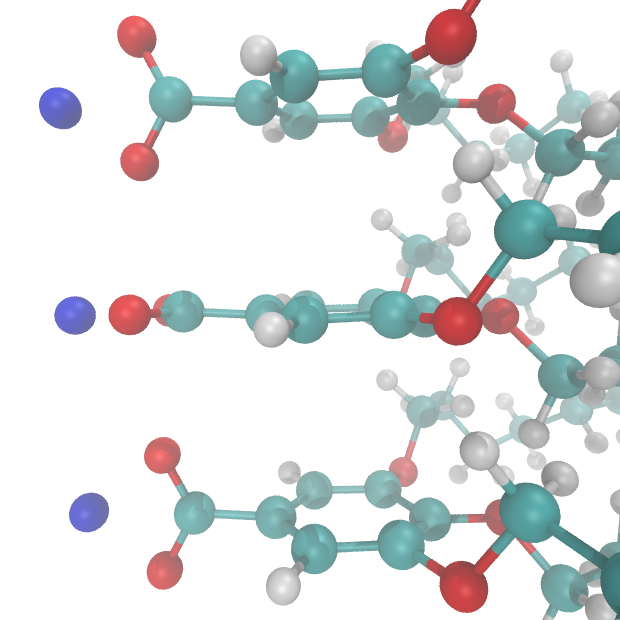
\includegraphics[width=\textwidth]{rotated_carboxylate.png}
%	\label{fig:rotated_carboxylate}
%  \end{subfigure}
  \begin{subfigure}{0.325\linewidth}
  	\centering
  	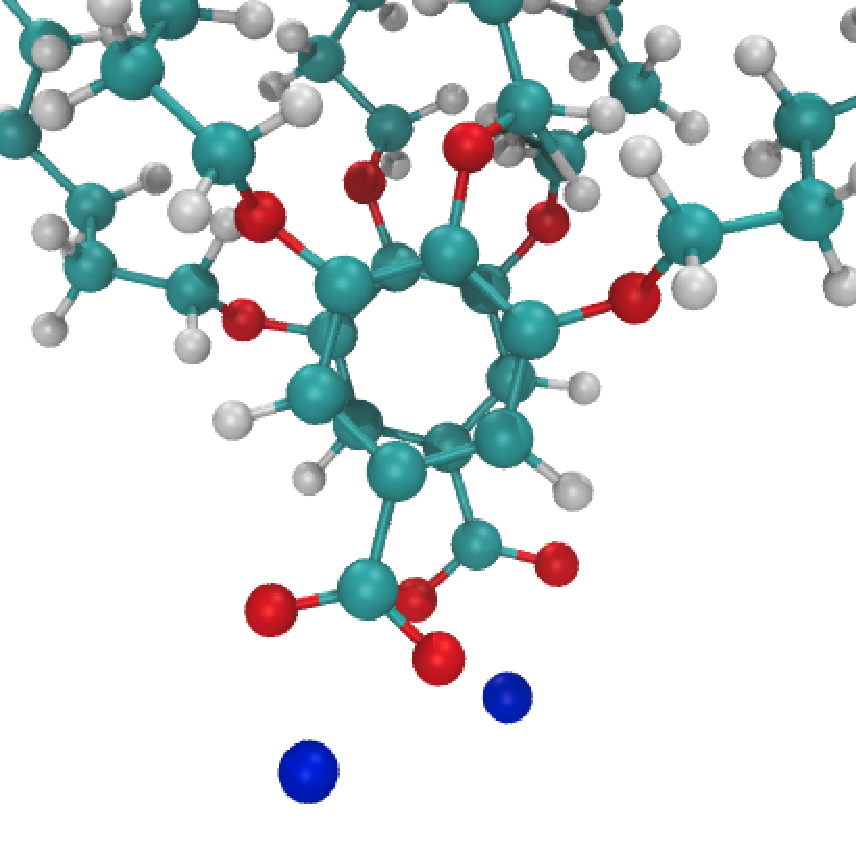
\includegraphics[width=\textwidth]{rotated_monomers.pdf}
  	\label{fig:rotated_monomers}
  \end{subfigure}
  \begin{subfigure}{0.325\linewidth}
  	\centering
  	\includegraphics[width=\textwidth]{staggered.pdf}
	\label{fig:staggered}
  \end{subfigure}
  \begin{subfigure}{0.325\linewidth}
  	\centering
  	\includegraphics[width=\textwidth]{solvated_pore_cross_section.pdf}  %BJC6: I can simplify this more (stacked monomers on each side with a few water molecules in between.
  	\label{fig:solvated_pore}
  \end{subfigure}
%  \begin{subfigure}{0.3\linewidth}
%  	\centering
%  	\includegraphics[width=\textwidth]{rotated_carboxylate_rzplot_restrained.png}
%  	\label{fig:rotated_carboxylate_rzplot_restrained}
%  \end{subfigure}
  \begin{subfigure}{0.325\linewidth}
  	\centering
  	\includegraphics[width=\textwidth]{rotated_monomers_rzplot_restrained.pdf}
  	\label{fig:rotated_monomers_rzplot_restrained}
  \end{subfigure}
  \begin{subfigure}{0.325\linewidth}
  	\centering
  	\includegraphics[width=\textwidth]{staggered_rzplot_restrained.pdf}
  	\label{fig:staggered_rzplot_restrained}
  \end{subfigure}
  \begin{subfigure}{0.325\linewidth}
  	\centering
  	\includegraphics[width=\textwidth]{solvated_pore_rzplot_restrained.pdf}
  	\label{fig:solvated_pore_rzplot_restrained}
  \end{subfigure}
%  \begin{subfigure}{0.3\linewidth}
%  	\centering
%  	\includegraphics[width=\textwidth]{rotated_carboxylate_rzplot_norestraints.png}
%  	\caption{}\label{fig:rotated_carboxylate_rzplot_norestraints}
%  	%BJC4: needs to run longer
%  \end{subfigure}
  \begin{subfigure}{0.325\linewidth}
  	\centering
  	\includegraphics[width=\textwidth]{rotated_monomers_rzplot_norestraints.pdf}
  	\caption{}\label{fig:rotated_monomers_rzplot_norestraints}
  \end{subfigure}
  \begin{subfigure}{0.325\linewidth}
  	\centering
  	\includegraphics[width=\textwidth]{staggered_rzplot_norestraints.pdf}
  	\caption{}\label{fig:staggered_rzplot_norestraints} 
  \end{subfigure}
  \begin{subfigure}{0.325\linewidth}
  	\centering
  	\includegraphics[width=\textwidth]{solvated_offset_rzplot_1.pdf}
  	\caption{}\label{fig:solvated_pore_rzplot_norestraints}
  \end{subfigure}
  \caption{(a) When monomer head groups are rotated with respect to vertically
	  adjacent monomers (top), R-double is visible while the heavy atoms of the head
	  groups are held in place with position restraints (middle). R-double
	  fades once the position restraints are released. (b) When monomers are
	  non-uniformly spaced (top), R-double appears if all heavy atoms of the head
	  groups are held in place with position restraints (middle). R-double quickly
	  fades once the position restraints are released (bottom). (c) When we add 1
	  wt\% water to the parallel displaced configuration in the ordered basin (top)
	  R-double is not initially present during the restrained portion of
	  equilibration (middle).  After 200 ns of equilibration, R-double becomes
	  visible and persists for another 200 ns (bottom).}\label{fig:rdouble}
  \end{figure}

  R-double appears in the solvated system due to the structuring of the head
  groups. To demonstrate this, we removed the head groups from the trajectory
  used to produce Figure~\ref{fig:solvated_pore_rzplot_norestraints} in order to
  produce that shown in Figure~\ref{fig:rdouble_nophenyls}. R-double does not
  appear without the presence of the head groups. Water molecules must therefore play a
  role in the structuring of the head groups in these simulations since R-double does not appear in
  any dry simulations.

  When two vertically stacked monomer head groups hydrogen bond with a shared
  water molecule, the monomers are drawn closer together (as illustrated in
  Figure~\ref{fig:hbond_visualization}), which creates an asymmetry that allows
  R-double to appear. If a monomer head group shares a hydrogen-bonded water
  molecule with a head group above itself, it will be less likely to share a
  water molecule with a head group below it due to geometric constraints. The
  monomer head group below can just as easily share a water molecule with a head
  group below itself. In this scenario, the COMs of each pair are 2 times the
  $\pi$-stacking distance apart which would lead to R-double (much like the
  configuration in Figure~\ref{fig:staggered_rzplot_norestraints}). There are a
  modest number of occurrences of this scenario, which we quantify in further
  detail in the SI, Section \ref{S-section:rdouble}.  
  
  Of all the configurations tested, it is most likely that R-double is induced
  by water molecules as described above since it is the only mechanism that can
  be observed without position restraints. The extent of the hydrogen-bonded
  network that forms is largely determined by the accuracy of the forcefield. It
  is possible that a more realistic force field would make the effect stronger or
  weaker. If this is truly the mechanism, it implies that the system studied by
  Feng et al.\cite{feng_scalable_2014,feng_thin_2016} was not truly a
  thermotropic Col\textsubscript{h} phase. Rather, they were very low water
  content H\textsubscript{II} phases unintentionally created due to the neat
  monomers' hydroscopicity.  Anecdotal evidence from other researchers suggests
  that membranes are less likely to assemble under completely dry
  conditions, supporting the idea %~\cite{personal_communication_with_mike_mcgrath} <- BJC16: what do I do with this?
  that the ``dry'' structures do absorb some water. This detail may therefore be
  important for reproducing the results of Feng et al.

  \begin{figure}[!htb]
  \begin{subfigure}{0.45\textwidth}
  \centering
  \begin{subfigure}{\textwidth}
  \includegraphics[width=\textwidth]{nophenyls_rzplot.pdf}
  \end{subfigure}
  \caption{}\label{fig:rdouble_nophenyls}
  \end{subfigure}
  \begin{subfigure}{0.45\textwidth}
  \centering
  \includegraphics[width=\textwidth]{hbonds_tails.pdf}
  \caption{}\label{fig:hbond_visualization}
  \end{subfigure}
  \caption{(a) The structure of the head groups is responsible for the appearance of
  R-double. When we remove head groups from the trajectory, the simulated 
  diffraction pattern no longer shows R-double. (b) Monomer head groups above or below
  each other that hydrogen bond with a shared water molecule are drawn closer
  together in the $z$-direction. Blue monomers were stacked above orange monomers in the
  initial configuration.}\label{fig:hbonds}
  \end{figure}
  
  \subsection{Atomistic structure of the pore columns}

  We are most interested in the structure and composition of the pores since we
  would like to study transport mechanisms within them. We have shown that the
  tails possess a certain degree of order which is necessary in order to create
  the complex WAXS pattern shown experimentally, but they will not be involved in
  a separation process. We aim to further understand the pore architecture, in
  order to address Question~\ref{point:composition} posed in the Introduction, 
  and observe the differences, if any, between the different plausible equilibrated
  configurations studied so far. In general, the composition of each region, particularly within our
  definition of the pore region, is similar between all systems. This suggests
  that the details of transport may be relatively independent of the structural
  differences between different possible structures studied here.

  We plotted the number densities of heavy atoms in the head group, carbon atoms in the tail
  region and all sodium ions (Figure~\ref{fig:overlaid_densities}). For the head group
  region, we used heavy atoms making up the aromatic rings and carboxylate groups. For the tail
  region, we used carbon atoms of the monomer tails (See Figure \ref{S-fig:monomer_color_coded}
  of the SI for a diagram). We averaged the histograms over the equilibrated
  portion of the trajectory. 
  There is a gradient in pore composition transitioning radially from the hydrophilic 
  to the hydrophobic region, rather than an abrupt division. Based on size-exclusion 
  experiments, the pore radius was estimated to be 0.6 nm~\cite{zhou_supported_2005}. 
  However, the simulations do not confine
  sodium ions and head groups to just within this experimentally-defined pore region. For dry systems,
  19\% of sodium ions exist outside the pore region (except sandwiched, ordered basin,
  where 16\% are outside the pore). Additionally, in all cases, about 
  3\% of the plotted tail density is located within the pore region (except ordered sandwiched,
  where 1.5\% are within the pore region). For the solvated system, the results are similar,
  however the head group density is shifted slightly radially outward, due to
  swelling of the pore by water. 

  The space in the pore region is filled with a mixture of sodium ions
  and head groups. The distributions appear somewhat different near r=0, but noise 
  is higher since there is significantly less sampling as r approaches 0. Regardless, 
  all systems, including the solvated system, have a significant number of head groups 
  and sodium ions occupying the pore center. This observation highlights that the pore
  region is dense, not hollow, and may impede transport of solvent and solutes when
  compared to the previous idealized picture of a hollow tube conducive to transport.
  
  \begin{figure}[!htb]
  \centering
  \begin{subfigure}{\textwidth}
  \includegraphics[width=\textwidth]{regional_density_legend.pdf}
  \end{subfigure}
  \begin{subfigure}{0.32\textwidth}
        \includegraphics[width=1\linewidth]{sodium_density.pdf}
        \caption{Sodium Ions}
        \label{fig:sodium_regional_density}
  \end{subfigure}
  \begin{subfigure}{0.32\textwidth}
        \includegraphics[width=1\linewidth]{head_group_density.pdf}
        \caption{Head Groups}
        \label{fig:head_groups_regional_density}
  \end{subfigure}
  \begin{subfigure}{0.32\textwidth}
        \includegraphics[width=1\linewidth]{tails_density.pdf}
        \caption{Tails}
        \label{fig:tails_regional_density}
  \end{subfigure}
  \caption{In all cases, the component radial distribution functions are similar. 
      They exhibit a composition gradient transitioning from the hydrophilic to the hydrophobic
	  regions. The biggest differences are at r=0 where noise is higher due to 
	  decreased sampling. The center of the pore is not hollow, but contains sodium ions and 
	  head groups, even when the system is solvated. This architecture may impede transport in 
	  the real system in a chemically-dependent manner. 
          The solvated system has a lower density of head groups near the 
	  pore center which is likely due to the swelling that is necessary in order to fit water
	  molecules in the pore region.}~\label{fig:overlaid_densities}
  \end{figure}

  \subsection{Slow dynamics}\label{section:slow_dynamics}
  
  We observe slow dynamics in our system. Typical diffusion constants for
  columnar liquid crystals have been reported to be between $10^{-11}~
  \mathrm{m}^2/\mathrm{s}$ \cite{dong_translational_1984} and
  $10^{-14}~\mathrm{m}^2/\mathrm{s}$ \cite{dvinskikh_molecular_2002}.  In the
  case of LLCs, we would expect a diffusion coefficient at the low end of this
  range since hydrophilic regions of monomers can hydrogen bond, thus increasing
  the energetic barriers for motion. We measured the diffusion constants of
  monomers in each of the main systems we studied (see Table \ref{S-table:msd} of
  the SI) and find they are all on the order of
  $10^{-14}~\mathrm{m}^2/\mathrm{s}$. However, since on this timescale, no
  monomers move a full `level' above or below, this may be an overestimate. This
  slow speed is not entirely surprising considering how densely the monomers are
  packed as implied by diffraction experiments. The entangled tails likely
  restrict both vertical and lateral movement.

  Consequently, there is not enough movement on the timescales we simulated for
  the system to consistently reach a definitive equilibrium structure. In all
  cases our monomers equilibrate to a stacking distance that is too large
  compared to experiment.  As discussed in Section~\ref{section:rpi}, while this
  may be in large part due to the force field's inability to model aromatic
  interactions, it is also possible that the monomer tails do have enough time to
  pack as tightly as they could. More densely packed tails could allow the
  monomers to stack closer together. 
  
  We quantified the movement of the tails during our simulations by calculating the 
  autocorrelation function of the dihedral angle formed around the bond between the 
  head groups and the ether oxygens which attach the tails to the head group 
  (see Figure \ref{S-fig:dihedrals} of the SI). We exclude the dihedral from the middle tail 
  since it is fundamentally different than the two symmetric outside tails. We 
  limited these studies to the sandwiched configuration for simplicity.
  
  The ether dihedrals become decorrelated on a reasonable timescale when we raise
  the system temperature. At 300 K (Figure~\ref{fig:dihedrals_300K}), the autocorrelation function does
  not cross the $x$-axis until $\sim$105 ns meaning that tails fully rotate on average about 
  4 times over the course of the 400 ns that we studied. Additionally, the correlation 
  function plateau's near a value of -0.2 which indicates that the tails are starting in 
  an unfavorable configuration. We implemented distance restraints between the centers of 
  mass of monomer head groups to preserve the hexagonal phase, then raised the temperature 
  of the equilibrated 300 K ordered basin sandwiched system to 500 K. We witnessed 
  decorrelation of the ether dihedrals after $\sim$11 ns with a plateau at 0, 
  (Figure~\ref{fig:dihedrals_500K}) indicating a complete loss of memory. We annealed
  the resultant configuration back down to 300 K over 200 ns to see if the increased rotational
  freedom might allow the system to relax into to a more tightly packed configuration.
  
  Decorrelating the ether dihedrals at high temperature, followed by thermal annealing
  does not improve packing in our model. In the ideal case, if all monomers stacked 
  3.7 \AA~ apart, the $z$-dimension of our unit cell should be 7.4 nm. In the ordered basin, 
  sandwiched system studied in this paper, the $z$-dimension of the unit cell equilibrated 
  to 8.87 nm, which is roughly consistent with the stacking distance reported in 
  Table~\ref{table:correlation_length}. After 200 ns of annealing from 500 K to 300 K, the 
  $z$-dimension of the unit cell was 9.22 nm. We repeated the annealing procedure over the 
  course of 400 ns and the final z-dimension of the unit cell was 9.20 nm. Much longer
  annealing simulations may get the system to the correct density, but such simulations are beyond
  the scope of the current study.

  \begin{figure}[!htb]
  \centering
  \begin{subfigure}{0.45\textwidth}
  	\centering
  	\includegraphics[width=\textwidth]{dihedral_autocorrelation_300K.pdf}
  	\caption{300K}\label{fig:dihedrals_300K}
  \end{subfigure}
  \begin{subfigure}{0.45\textwidth}
  	\centering
  	\includegraphics[width=\textwidth]{dihedral_autocorrelation_500K.pdf} % Run : torsions.py -t tethered_columns.xtc -g tethered_columns.gro (the appropriate dihedral is the default)
  	\caption{500K}\label{fig:dihedrals_500K}
  \end{subfigure}
  \caption{The outer tail ether dihedrals become decorrelated on a reasonable
  timescale when we raise the system temperature. (a) The dihedrals do not
  become decorrelated for ca. 100 ns when the system is equilibrated at 300 K.
  (b) The ether dihedrals become decorrelated after 11 ns when the temperature
  of the system is increased to 500 K.}\label{fig:dihedrals}
  \end{figure}
  
  \subsection{Ionic Conductivity Measurements}
  
  We calculated the ionic conductivity of the parallel displaced configuration in
  the ordered basin with 1 wt\% water since we believe its structure is the 
  closest match to experiment. Our model estimates the ionic conductivity to be
  $(5.92 \pm 0.05)\times$\num{e-5}~S/m, about 5 times higher than the experimental value of 
  $(1.3 \pm 0.1)\times$\num{e-5}~S/m. We verified the value calculated by the Nernst-Einstein
  relationship using the collective diffusion model\cite{liu_collective_2013} 
  (see Section \ref{S-fig:conductivity} of the SI). The values calculated by the 
  collective diffusion model agree with Nernst-Einstein values within error, 
  however there is a much higher uncertainty that would require much longer 
  simulations to lower.

  The calculated value of ionic conductivity is 5 times higher than experiment likely because 
  we simulated infinitely long, aligned pores. The ionic conductivity measurement 
  to which we are comparing was done with an \SI{80}{\micro\metre}-thick film, 
  nearly 10,000 times thicker than our simulated
  system. The thick film is likely imperfectly aligned and has defects leading to
  non-contiguous pores. It has been shown that there is a large dependence of 
  ionic conductivity on the alignment of the pores. The ionic conductivity of an
  isotropically aligned film is ca. 85 times lower than that of the nearly aligned
  film to which we are comparing~\cite{feng_scalable_2014}. We hypothesize that a 
  thin, perfectly aligned film would have a value of ionic conductivity in closer
  agreement with our model.

  \subsection{Effect of cross-linking}\label{section:xlink}

  Experimentally, membranes are cross-linked for mechanical stability before
  use. We applied our cross-linking algorithm to equilibrated sandwiched and
  parallel displaced configurations in the ordered pore basin. We allowed the
  cross-linking algorithm to propagate until greater than 90\% of the vinyl
  groups on the tails of the monomers were either involved in a cross-linking
  reaction or were terminated (see Section \ref{S-section:xlink} of the SI for
  further details of the cross-linking algorithm). We allowed the cross-linked
  configurations to simulate for 100 ns further in the NPT ensemble. 

  There are only minor changes to the physical characteristics of these systems when 
  they are cross-linked (See Figure~\ref{fig:xlink}). The ionic conductivity of 
  the sandwiched configuration decreases while that of the parallel displaced 
  configuration stays the same. The pore spacing decreases in both systems by
  0.07 nm. The vertical monomer stacking distance increases in the sandwiched
  configuration and decreases in the parallel displaced configuration, however the 
  values of cross-linked configurations fall within uncertainty of their un-cross-linked
  counterparts. The correlation length decreases in both systems, 
  but is most pronounced in the parallel displaced system.  
  
  \begin{figure}[!htb]
  \centering
  \includegraphics[width=\textwidth]{xlink_charts.pdf}
  \caption{There are minor differences between the physical properties of a
  crosslinked (xlink) system versus an uncrosslinked system. The sandwiched configuration (S)
  exhibits a smaller decrease in its ionic conductivity, while the parallel displaced (PD)
  configuration remains constant. The pore spacing of both systems decreases upon cross-linking.
  The vertical distance between stacked monomers increases in the sandwiched configuration
  and decreases in the parallel displaced configuration. The correlation length decreases
  in both configurations.}\label{fig:xlink}
  \end{figure}
 
  \section{Conclusions}
   
  We have used detailed molecular modeling of the Col\textsubscript{h} phase
  formed by Na-GA3C11 in order to study its nanoscopic structure. While there
  have been efforts to model formation of various liquid crystalline phases with
  molecular dynamics, to our knowledge there have been no studies which attempt
  to examine their structure with the same level of detail presented here.
  
  We observed a number of metastable configurations, stable for hundreds of 
  nanoseconds, which do not fit the experimental profile we have tried to match. 
  We explored two classes of metastable basins which are dependent on the initial
  vertical stacking distance between monomers: the ordered and disordered pore basins.
  We expect that these metastable configurations will eventually rearrange and converge
  to a single equilibrium structure. We conducted extensive analysis in order to 
  isolate structures which most closely resemble the true equilibrium structure.

  We achieve maximum structural consistency with experiment, as determined by
  simulated 2D-XRD patterns, when we build our model in the ordered basin
  parallel displaced configuration with 5 monomer columns per pore and 1 wt\%
  water. R-alkanes and R-pores appear where expected for the reasons originally
  predicted. We find that R-spots is likely due to ordered alkane chain packing.
  R-$\pi$ appears at lower $q_z$ values than experiment because monomer stack too far
  apart, and its intensity is far too high, likely because our initial
  configurations contain a high level of dependence between monomer columns.
  We can learn more about the time averaged structure of these systems by studying
  ensembles of independent simulations. Finally, we observed that our model can 
  only produce R-double when we add small amounts of water to the system. This 
  observation has possible implications for the reproducibility of the experimental
  results from Feng et al. since they specify that their membrane is synthesized dry.  

  We characterized the environment centered around the membrane pores and
  learned that the pores are generally filled with monomer head groups and sodium
  ions. All dry systems studied showed a similar distribution of sodium, head
  groups and tails while the wet system shows evidence of slight swelling, with
  minor changes in the distributions due to the presence of water molecules. We
  also observed that there is not a hard partition between hydrophilic and
  hydrophobic regions; instead, there is a gradient of chemical constituents. This finding raises
  questions about the nature of size-exclusion separations in systems without a
  well-defined pore size, which potentially could enable separations that
  vary with chemical identity as well as size. 

%  We learned that we do not need water to create well-defined pore structures.
%  Systems whose pores were filled with varying amounts of water showed a decrease
%  in structuring relative to dry systems. At higher water concentrations, the pores
%  begin to swell, which may be more conducive to transport.

  Our system can reasonably estimate ionic conductivity. Our
  calculations are about 1 order of magnitude higher than experiment, however
  that is to be expected since we are simulating a perfectly straight and
  defect-free membrane. 

  Finally, we verified that our conclusions do not change when the system is
  cross-linked by the algorithm we implemented. The ionic conductivity drops by a factor
  of $\sim$1.5, in closer agreement with experiment, the pore spacing decreases and
  the membrane becomes thicker; however, all changes are relatively minor, 
  preserving most of the features well.

  Future work, based on what has been learned in this study, may help further
  improve the structural agreement between experiment and simulation. Force 
  fields explicitly including $\pi-\pi$ interactions may be able to draw stacked
  monomers closer together. We can study ensembles of long simulations in order
  to observe more averaged structure and to create more experimentally consistent
  XRD patterns. Extremely long simulations (on the order of \SI{}{\micro s}) may
  be necessary to better quantify the time scales for large scale rearrangements,
  and the precise arrangements themselves.

  With the structural understanding gained by these simulations, it will be
  possible to evaluate transport of various solutes within the system, and apply the
  knowledge gained from this study in order to suggest improvements to the
  existing system, as well as to evaluate new unsynthesized LLC systems.

  \section*{Supporting Information}
  
  Detailed explanations and expansions upon the results and procedures mentioned in 
  the main text are described in the Supporting Information. This information is 
  available free of charge via the Internet at http://pubs.acs.org.

  \section*{Acknowledgements}

  J. Y. and M. A. G. were supported by the Soft Materials Research Center under NSF 
  MRSEC Grant DMR-1420736

  Molecular simulations were performed using the Extreme Science and
  Engineering Discovery Environment (XSEDE), which is supported by National
  Science Foundation grant number ACI-1548562. Specifically, it used the Bridges
  system, which is supported by NSF award number ACI-1445606, at the Pittsburgh
  Supercomputing Center (PSC). This work also utilized the RMACC Summit supercomputer,
  which is supported by the National Science Foundation (awards ACI-1532235 and
  ACI-1532236), the University of Colorado Boulder, and Colorado State
  University. The Summit supercomputer is a joint effort of the University of
  Colorado Boulder and Colorado State University.

  The authors thank Richard Noble, Michael McGrath, Gregory Dwulet and Sarah Dischinger
  for useful discussions that enhanced our understanding of these LC membrane systems. 

  \clearpage
  \bibliography{llc}
  
  \newpage
  
  \section*{Graphical TOC Entry}
  \begin{figure}
  \includegraphics[width=3.5in]{new_toc_graphic.pdf}
%  \includegraphics[width=4.5cm]{toc_image_final.pdf}
%  \includegraphics[width=4.07cm]{toc_waxs.pdf}
 \end{figure}

\end{document}

% LocalWords:  Nanostructured desalination biorefinement solute RO NF bruggen
% LocalWords:  polydisperse diffusivity solutes BJC ultrafiltration nanometer
% LocalWords:  ionizable pretreatment Graphene solvated Na GA zhou resel feng
% LocalWords:  ca wt mesophases al crosslinking THF nanoporous PDMS nanopores
% LocalWords:  TODO svg eps atomistically counterion nanoscopic counterions XRD
% LocalWords:  WAXS headgroups initio metastable timescales acessible leached
% LocalWords:  SAXS alkane alkanes Antechamber bccsym molcharge QUACPAC Openeye
% LocalWords:  Gromacs berendsen timescale Packmol xyz hydrophlic xy pd tshaped
% LocalWords:  KJ NVT kJ Parrinello Rahman gmx solvate polymerization FRP FRPs
% LocalWords:  crosslink binned DC MSD subharmonic matplotlib GAFF's xrd llc ab
% LocalWords:  polarizable reconcilable screenshot crosslinked uncrosslinked AA
% LocalWords:  nanofiltration permeability interfacial diamine polysulfone der
% LocalWords:  trimesoyl immiscible polymerizes etching Osuji's nanostructured
% LocalWords:  Donnan modelling nanotubes monodispersity maruyama Zeolites Col
% LocalWords:  lyotropic thermotropic png kinetically colorbar gromacs hess dr
% LocalWords:  gimp disassociate pore's barostat racemic colorbars Nernst LLCs
% LocalWords:  entropic rzplot transitioning spoel github pymbar Yelk Glaser xr
% LocalWords:  flowback FW wastewaters wastestream fracking semipermeable TFC
% LocalWords:  solute's polymerized wijmans diffusivities amphiphilic MWCO Ia
% LocalWords:  nanostructures bicontinuous hatakeyama tortuosity Pn hII TLC ing
% LocalWords:  microstructures multilayer Xunda's refamiliarize nanostructure
% LocalWords:  nanoscale TEM LC methacrylated Eq scipy equil xz meridional phys
% LocalWords:  semiisotropic nocbar chem waxs ish fb entropically steric vv rpi
% LocalWords:  highlimit yz nematically carboxylate norestraints rb Bushey cyan
% LocalWords:  dihedrals cbar adenine carboxyl sterically QM hydroscopicity LCs
% LocalWords:  nophenyls nowater hbonds notails decorrelated Decorrelating SI
% LocalWords:  xlink uncross
